In this chapter we describe a software framework called Rheos, which demonstrates an approach for reasoning about large genomic datasets utilizing concepts of service-orientation and data streaming in contrast with traditional genomic data analysis frameworks\autocite{depristo2011framework} that take a procedural batch-based approach. Our approach allows the users to make active tradeoff decisions between analysis time, cost, and quality as well as setting up precise operational Service Level Agreements, both between Rheos components, and between Rheos and external systems, as we describe below. We begin by describing a general framework of stream-based services and identify broad classes of such services based on their roles and capabilities. We use the general Rheos framework to implement several genomic data analysis use cases, namely germline SNP and Deletion variant calling. We scalably deploy Rheos onto an academic cloud computing environment running OpenStack and set up detailed monitoring to be able ensure operational control of the software at runtime. We conclude by testing Rheos on a real data set prepared by NIST's Genome In a Bottle Consortium and comparing the results with the results generated by several leading tools. We find that the initial Rheos implementation is quite comparable to other methods in accuracy (~98\% sensitivity, ~99\% specificity in SNP calling, ~85\% sensitivity and specificity in deletion calling), while allowing the user to actively control the tradeoff between time, cost, and quality, which isn't readily available to other tools. This establishes Rheos as an attractive and promising approach for large scale genomic analysis of the future. 

\section{General Framework Design}

As already discussed in Chapters \ref{ch:introduction} and \ref{ch:background}, the general problem consists of collecting DNA samples from a population of individuals under study, sequencing these samples using Next Generation Sequencing techniques, identifying the mutations that are present, annotating their functional impact and utilizing the obtained data in a downstream data analysis with research or clinical decision-making goals. While there is a great variety of possible downstream analyses that may be performed depending on the individual goals of the analyst, there is a fairly well established set of steps for processing of the raw NGS data into a set of annotated variants, and it is these steps that we target with this work. The typical approach that is in widespread use today is to collect a batch of samples and then process each sample individually with a sequence of separate tools, that may be described via a higher-level workflow construct (such as in Figure \ref{fig:gatk_best_practices}, or using a framework like Butler, as described in Chapters \ref{ch:butler_architecture}, \ref{ch:butler_implementation}). There are, however, a number of factors that leave room for improvement in this model. 

Data arrives from the sequencer as a random ordered collection of reads. These reads are mapped to a coordinate system of the reference genome. Reads are then sorted by coordinate and individual variant callers traverse the data set in a coordinate-wise fashion to perform the analysis. See Chapter \ref{ch:background} for more details on this process. This approach implies that data needs to be mapped before it is sorted, and sorted before it is variant called, which means that a single sample (Which can be anywhere between 150-300 GB in size currently) is traversed completely at least 4-5 times before any meaningful results are obtained. Additionally this implies that decisions need to be made up front about how much data to sequence, and analyze which virtually fixes the cost, time, and quality of the analysis before any data is seen. If we are able to abandon this approach in favour of a dynamic online integration of new data as it becomes available we open up the opportunity to achieve greater efficiency (because we are not waiting for the entire data set to be processed in one stage before going on to the next), and enable the active tradeoff between cost, time, and quality based on the data that is being observed. Since we progressively elaborate our data set as new data becomes available, we can choose to cut off our observations early if we achieved a desired quality level, or observed an event of interest (thus reducing time and cost), or we can choose to end an analysis by a certain time point and accept the results that have been achieved up to that point. 

\begin{figure}[H]
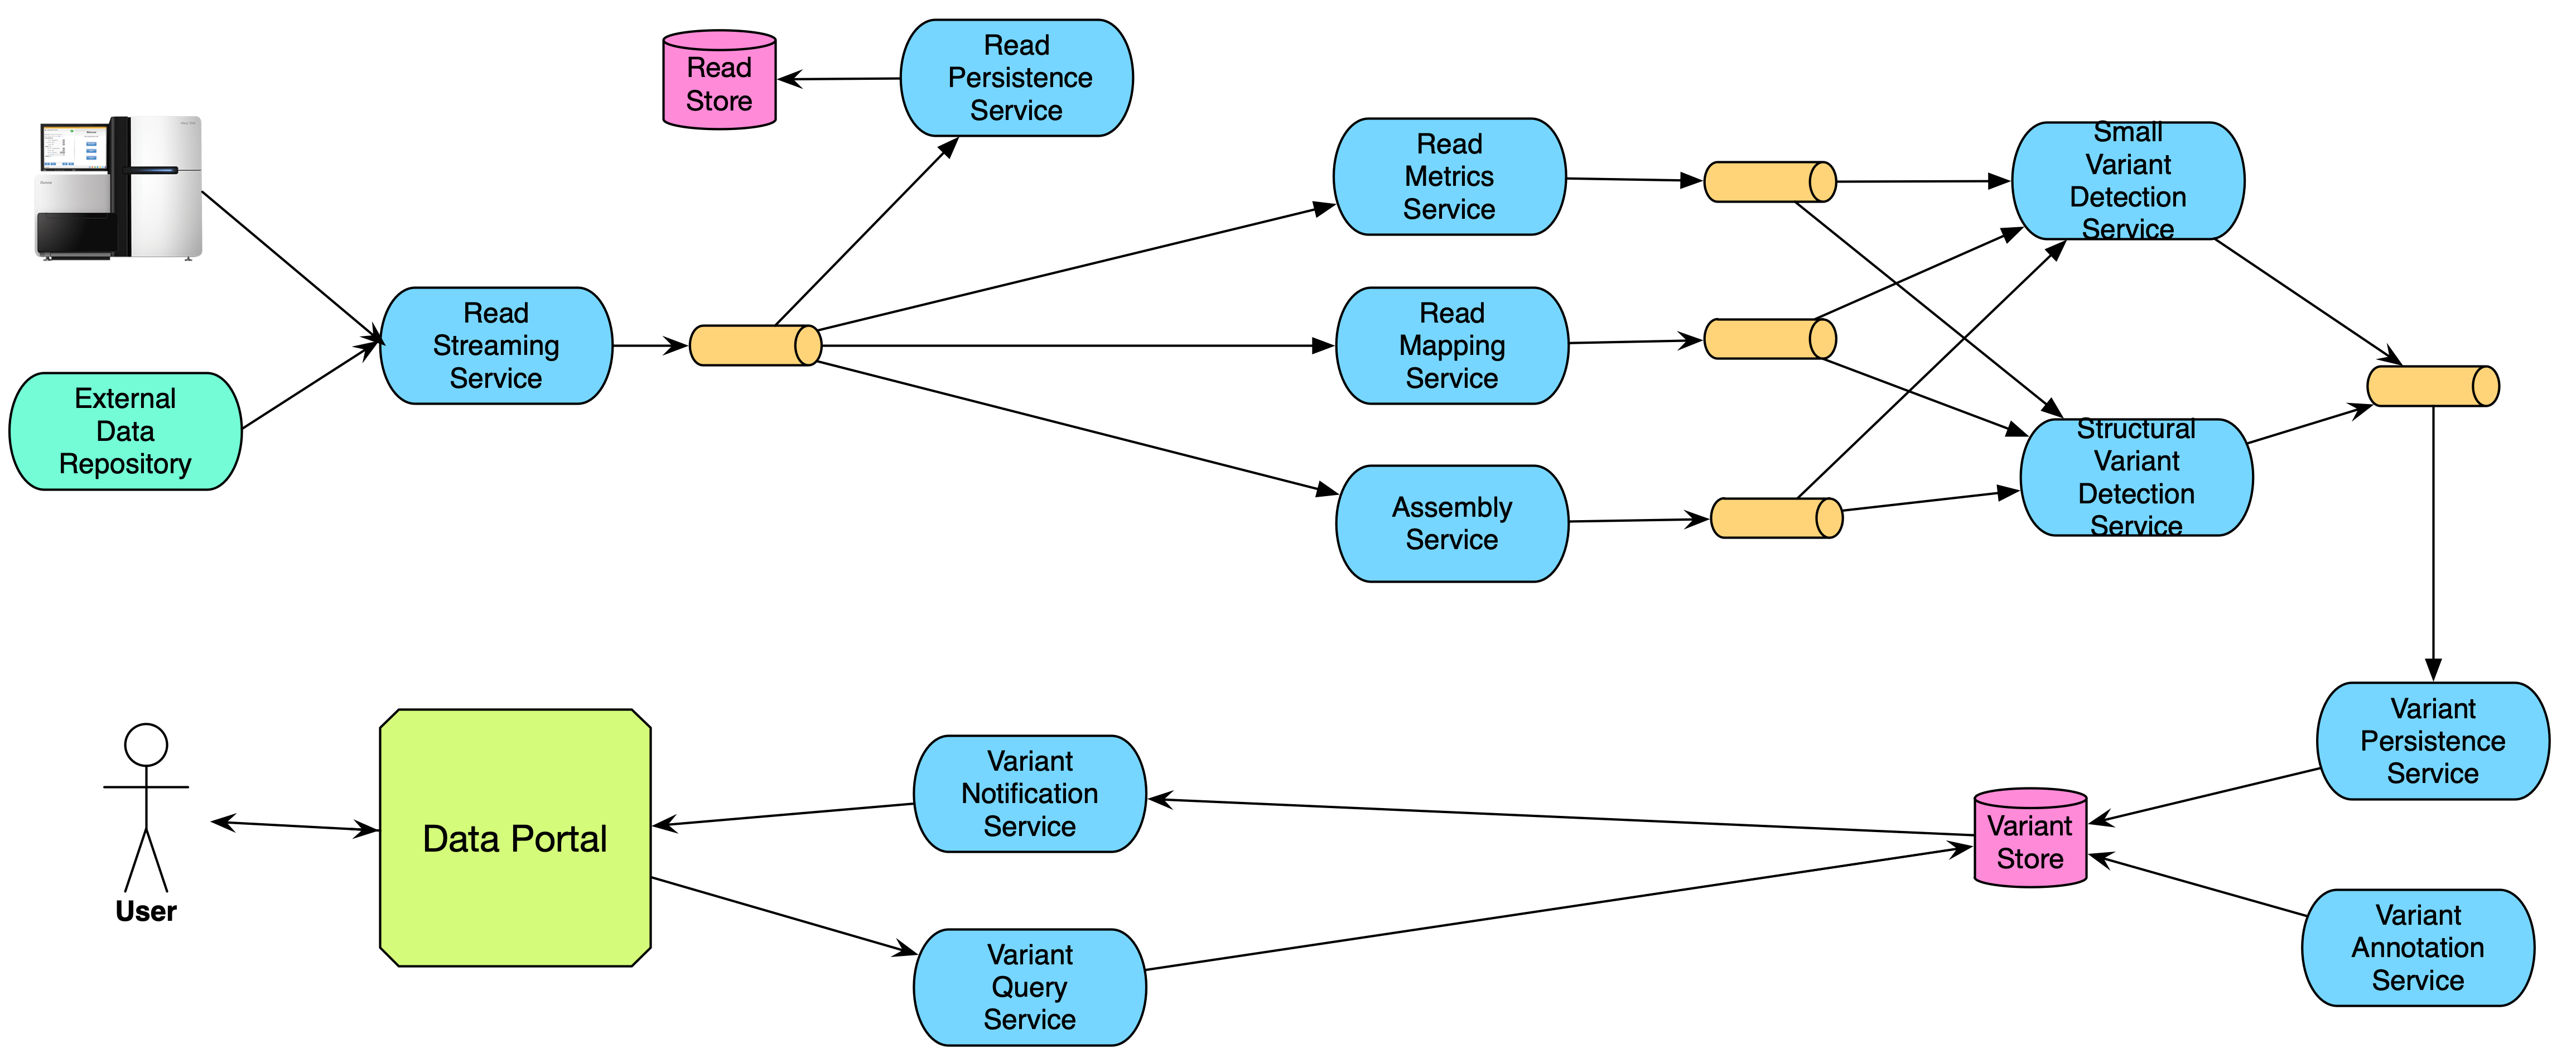
\includegraphics[scale=0.38]{rheos_high_level}
\centering
\caption {High level architecture of the Rheos framework.}
\label{fig:rheos_high_level}
\end{figure}

This approach requires a new framework for genomic data processing as a continuous stream of data, because the current batch-based toolset is focused on processing entire files and doesn't allow real-time dynamic decision making about cost and accuracy. Additionally, a suite of new algorithms for online analysis is required, because core assumptions of currently existing algorithms are broken when data is not all available at the same time, and when it arrives in random order, rather than being coordinate-sorted. The general high level architecture of the Rheos framework the we have created to answer these challenges is depicted in Figure \ref{fig:rheos_high_level}. Each blue bubble is a service - an encapsulated collection of data processing capabilities that operates on a stream of data and has well understood runtime characteristics that can be dynamically controlled. Each orange pipe is a distributed queue that stores stream-based data in-flight and facilitates routing of information through the system. There are data stores established for data persistence where necessary, and a data portal to facilitate interaction with users.

The interface between existing file-based systems and the new stream-based Rheos system occurs at the Read Streaming service. This is where data is read from a traditional data source like a BAM file, and is transformed into a stream of reads. Useful metrics about the reads are collected by the Read Metrics Service. The reads are mapped to a reference genome using the Read Mapping Service and flow over to variant calling at the Small Variant and Structural Variant Detection services. Variants are persisted to a data store and are accessible to the user via the Data Portal both in pull model where the user can query specific variants, and in a push model where the user is notified about the identification of variants of interest. Each variant calling service maintains a set of models about the sample under analysis that are progressively elaborated as new data arrives. We measure the capacity of each service to perform its operations and increase and decrease resource allocation based on required throughput. 

Since in this framework we are able to continuously integrate new data, measure outcome accuracy, and dynamically allocate resources based on desired operating characteristics, this establishes the overall set of capabilities that we set out to achieve. We dedicate the rest of this chapter to a detailed discussion of the Rheos framework architecture, design of individual services, their implementation, deployment, and experimental validation on a real data set.


\section{Data Streaming Architecture}
\label{sec:rheos_streaming_architecture}

The overall technical architecture of the Rheos system is set up as a Service Oriented Architecture (SOA)\autocite{shaw1996software} which is an information system architecture paradigm where the overall problem that the system is trying to solve is broken down into a collection of loosely-coupled components called services. Each service has a well defined interface of inputs that it accepts and outputs that it produces. Services can be combined and orchestrated together to produce the overall desired output for the system. A key distinguishing feature of this architectural approach is that each service can be individually optimized to fulfill its contract most efficiently helping break down some of the performance limitations brought about by the necessity to simultaneously tackle competing constraints in more monolithic information system designs. Additionally, within a services framework, the dependencies between separate services can be negotiated not only in terms of service interfaces, but also in terms Service Level Agreements which constitute Quality of Service promises made by one service to its dependents\autocite{ingham2000constructing}. Because it is unlikely that a service designer will be able to accurately foresee all of the demands that will be placed on a service during its lifetime the SLAs provide a valuable feedback framework through which the service can be evaluated as it operates in production, as well as serving as a basis for negotiating evolving requirements between dependent services.

While general web services can support any data processing paradigm, in the Rheos framework we adopt a data streaming approach\autocite{babcock2002models}. In this approach we assume that the input to any service is a randomly ordered sequence of messages $M = {m_1, m_2, ....}$ where each message represents a fact about the underlying domain that the service reasons over, as well as some metadata, including an identifier, and a variety of timestamps of interest. The content of each message may provide a datum, such as the measurement of a quantity of interest, or signal that a particular event has taken place. It is in general assumed that the data stream is infinite in size, that messages may arrive out of order, and that any message that is placed in the stream is observed at most once, and may, in fact, never be observed. Messages are typically not sent directly from one service to another, instead the transfer of messages is mediated by a queuing system using a publish-subscribe\autocite{eugster2003many} model. Under this model each queue acts as a \emph{topic}. Message producers can publish data to the topic, and message consumers subscribe to receive messages from the topic. A message is consumed from the queue only after all of the subscribed consumers have seen it. End users retrieve information from the system via a set of User Interfaces that support both push (notifications) and pull (querying) models of data retrieval. A more detailed description of the architectural aspects of the system follows:

\subsection{Service-Oriented Data Streaming Model}
\label{sec:rheos_data_streaming_model}

A data stream $M_{s,d} = {m_1, m_2, ....}$ is a sequence of datagrams transmitted over the network with the following properties:

\begin{itemize}
    \item The stream has a source $s$ and a destination $d$.
    \item A message $m$ in the stream is a tuple of the form $(header, payload)$, where:
    \begin{itemize}
        \item $header$ is a tuple of the form $(id, \dots)$ that holds at minimum a unique identifier $id$ for messages, and may hold additional metadata.
        \item $payload$ is an arbitrary data structure that holds the informational content of the message. 
    \end{itemize}
    \item $|M| = \infty$ by assumption.
    \item Messages may not arrive at destination $d$ in the same order that they were sent from source $s$.
    \item If $t_{i,s}$ is the time message $m_i$ leaves the source $s$ and $t_{i,d}$ is the time of arrival at destination $d$, then $\sup_i \{t_{i,d} - t_{i,s}\} = \infty$, i.e. a given sent message may never arrive at its destination.
\end{itemize}

A service $S = \{o_i\}$ is a collection of operations $o_i$ that act on one or more input data streams $\{M_i\}$ to produce one or more transformed output data streams $\{M_j\}$. Specifically:

An operation $O$ is a tuple of the form:

\begin{equation}
\label{eq:service_opertaion_equation}
O = (i,o,p,f)
\end{equation} 
where:
\begin{itemize} 
    \item $i = \{M_j, j \in [0, K]\}$ is a set of $K \ge 0$ input data streams.
    \item $o = \{M'_j, j \in [0, L]\}$ is a set of $L \ge 0$ output data streams.
    \item $f:M^K \mapsto M'^L$ is a transformation function that produces messages $m'$ in the output streams based on messages $m$ observed in the input streams.
    \item $p = \{p_i\}$ is a set of potentially optional query parameters.  
\end{itemize}

There are several distinct categories of operations that a service can perform on a set of input streams. We describe these here:

\paragraph{Windowing Function} - Service $S$ observes a sliding window, which is a sample of size $n$ of messages from stream $M_i$ and computes a summary statistic (see Figure \ref{fig:stream_window_function}) over the sample which is meant to be an approximation of the corresponding population parameter.

\begin{figure}[H]
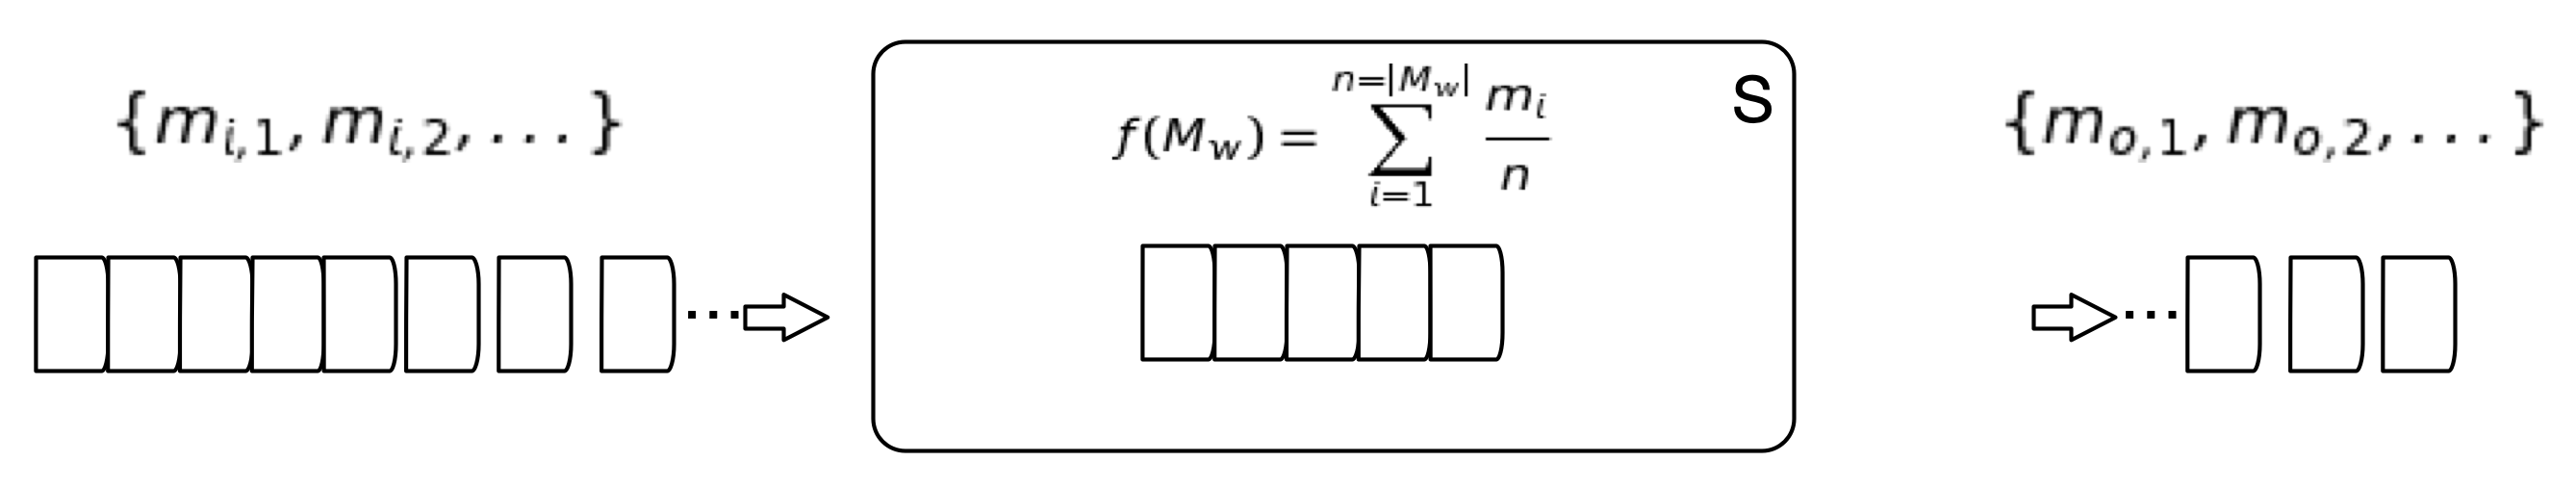
\includegraphics[scale=0.6]{stream_window_function}
\centering
\caption {Service S computes a summary statistic over a window of messages from stream $M$}
\label{fig:stream_window_function}
\end{figure}
 
\paragraph{Decorator Function} - Service $S$ observes messages $m_i$ and applies a function that augments (decorates) each message with additional attributes (see Figure \ref{fig:stream_decorator_function}) producing augmented messages $m_o$ as output.

\begin{figure}[H]
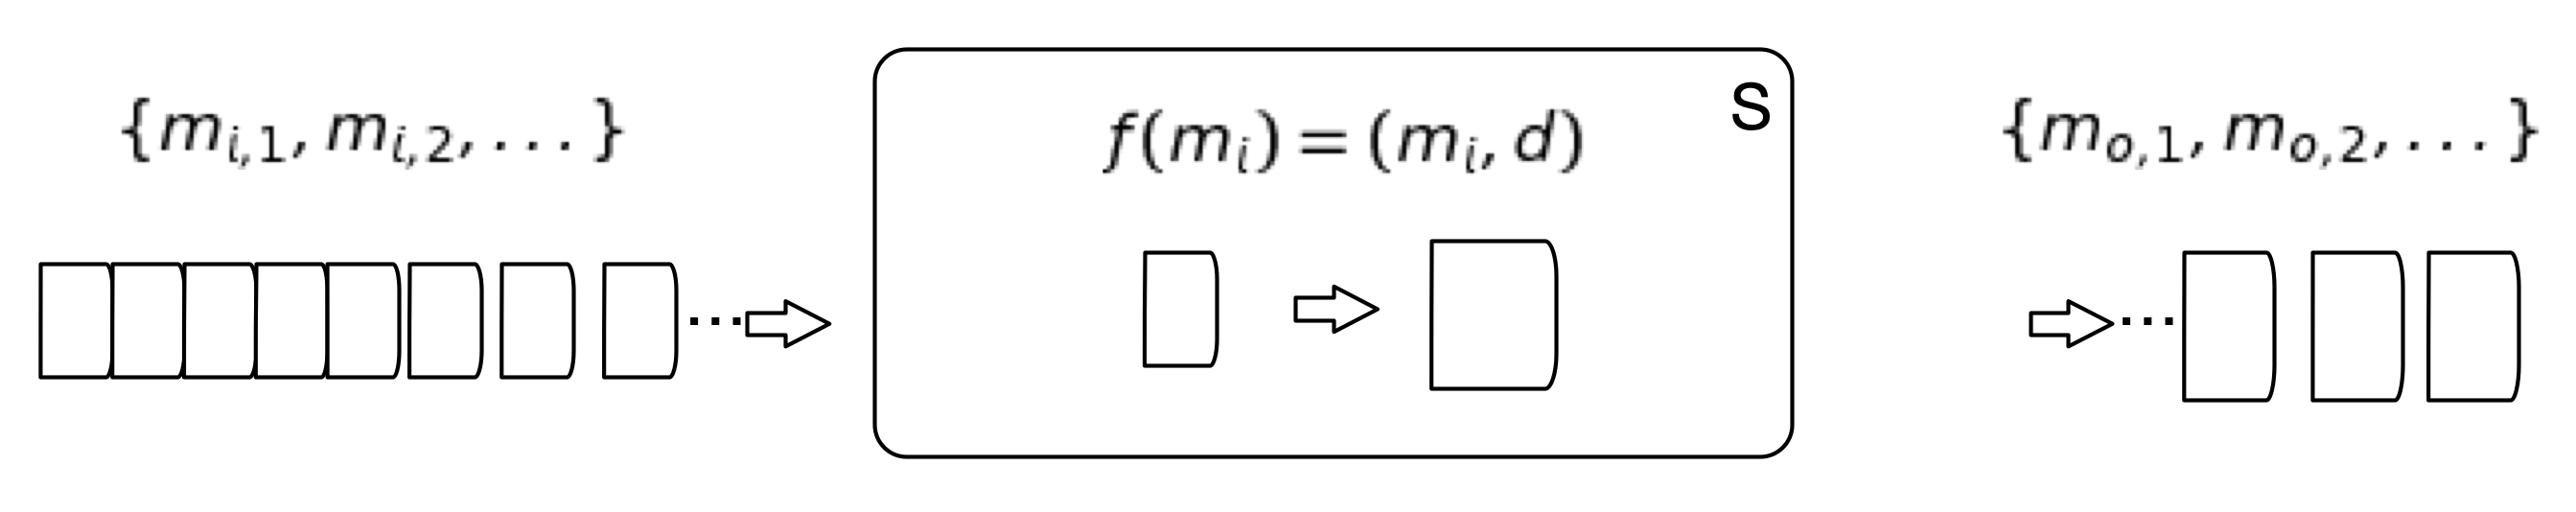
\includegraphics[scale=0.6]{stream_decorator_function}
\centering
\caption {Service S augments messages from $M$ with an additional set of attributes.}
\label{fig:stream_decorator_function}
\end{figure}

\paragraph{Filter Function} - Service $S$ observes messages $m_i$ and applies a function $f:M\mapsto\{True,False\}$ that evaluates to a boolean value (see Figure \ref{fig:stream_decorator_function}). Only messages that map to $True$ are emitted as output.

\begin{figure}[H]
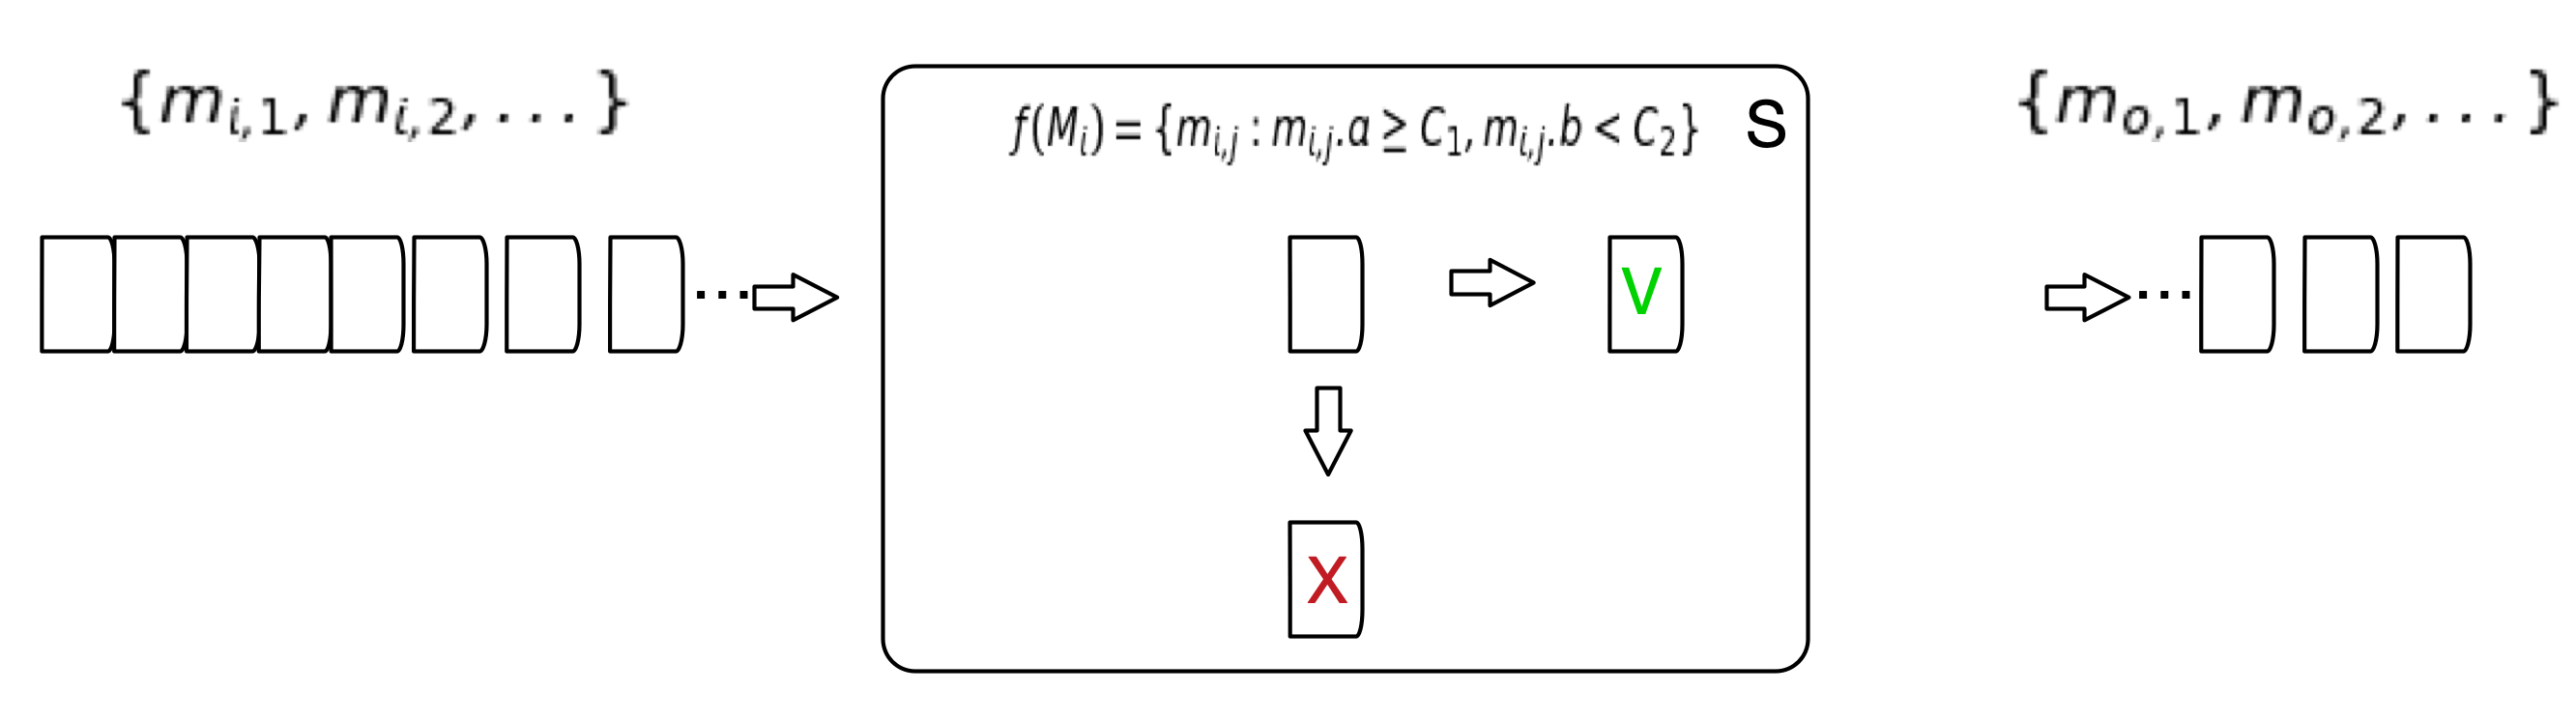
\includegraphics[scale=0.6]{stream_filter_function}
\centering
\caption {Service S filters messages from input stream $M$ and only allows through those that pass the filtering condition.}
\label{fig:stream_filter_function}
\end{figure}

\paragraph{Aggregator Function} - Service $S$ observes messages from $N$ different streams $\{M_j: j \in [1,N]\}$ and applies a function $f:M_i^N \mapsto M_o$ that aggregates messages from these streams to produce its output (see Figure \ref{fig:stream_aggregator_function}). Because aggregation happens over groups of messages that may not all arrive at the same time the service $S$ requires a mechanism for keeping local state so that it can accumulate messages that have already arrived while waiting for those that are necessary to compute $f$ yet have not been observed. The statefulness requirement of this type of service places an extra level of complexity (related to state-management and request routing) as well as inherent scalability limitations compared to stateless services\autocite{oppenheimer2002architecture}.

\begin{figure}[H]
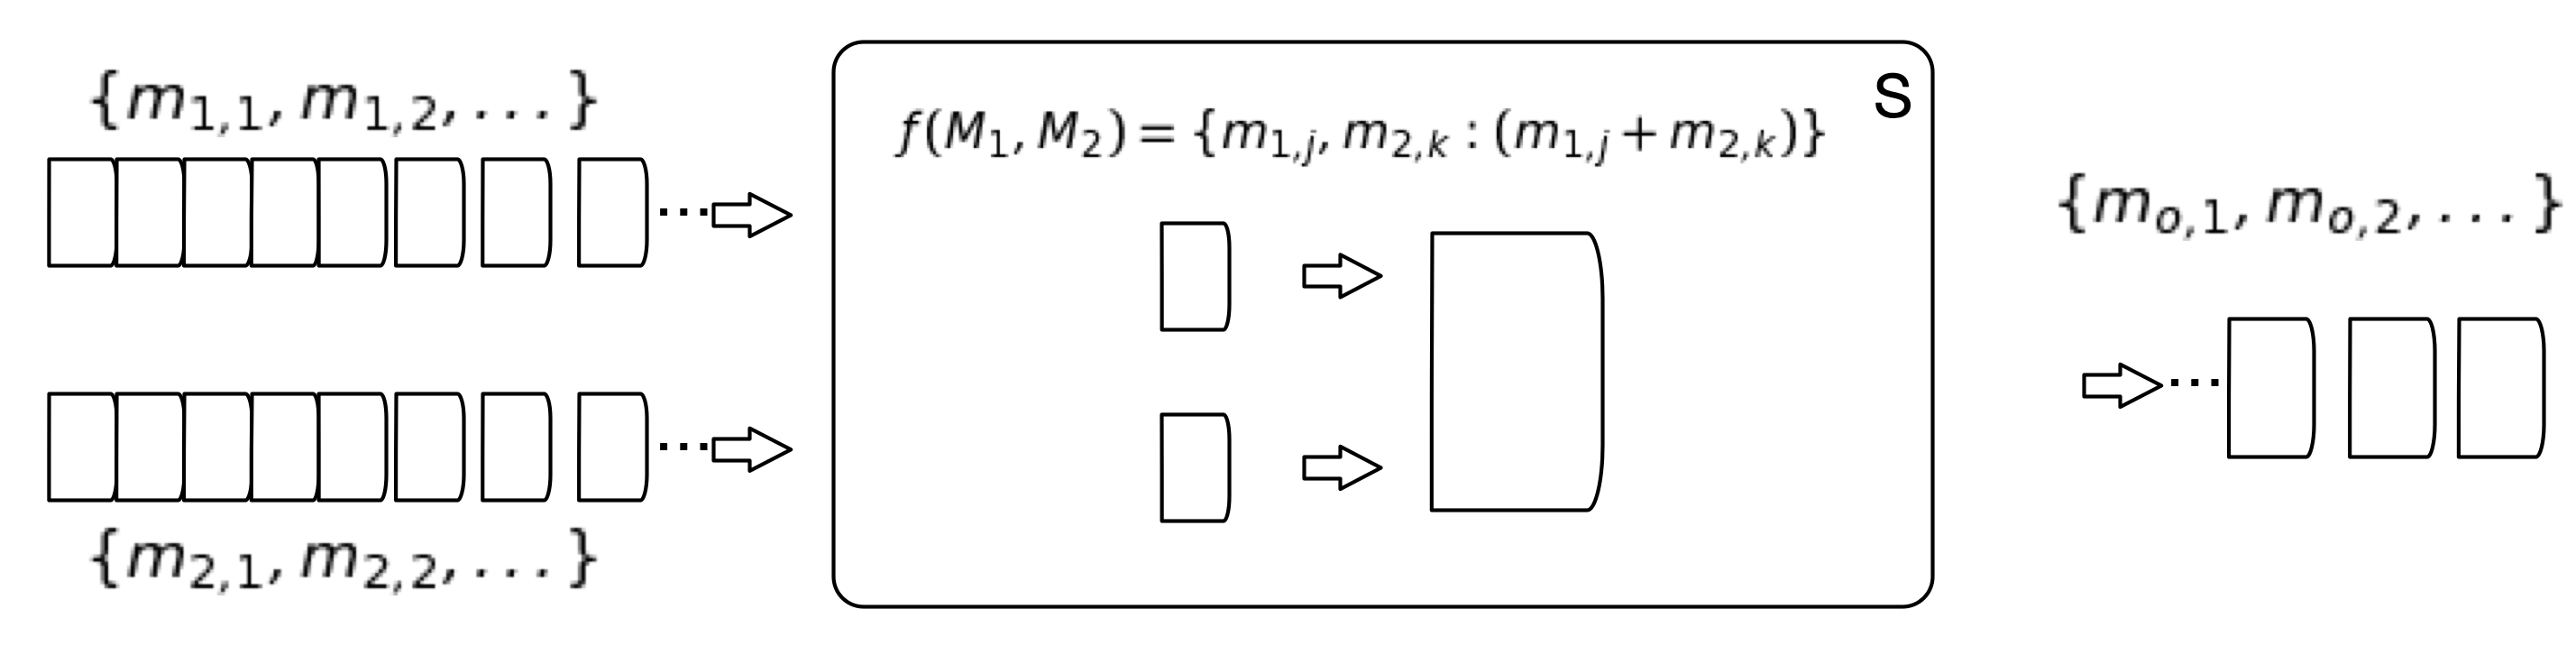
\includegraphics[scale=0.6]{stream_aggregator_function}
\centering
\caption {Service S integrates messages from multiple input streams $M_i$ to produce an aggregated output stream $M_o$ via $f$.}
\label{fig:stream_aggregator_function}
\end{figure}


\paragraph{Local State Aggregator Function} - Service $S$ observes an input stream $M_i$ which it integrates with a local (non-stream) queryable data store (see Figure \ref{fig:stream_local_state_aggregator_function}). Messages $m_i$ are integrated with query results $q_i$ to produce an output stream $M_i$. This type of service also requires management of state and scalability concerns similar to the Aggregator service, especially when the local data store is itself distributed. 

\begin{figure}[H]
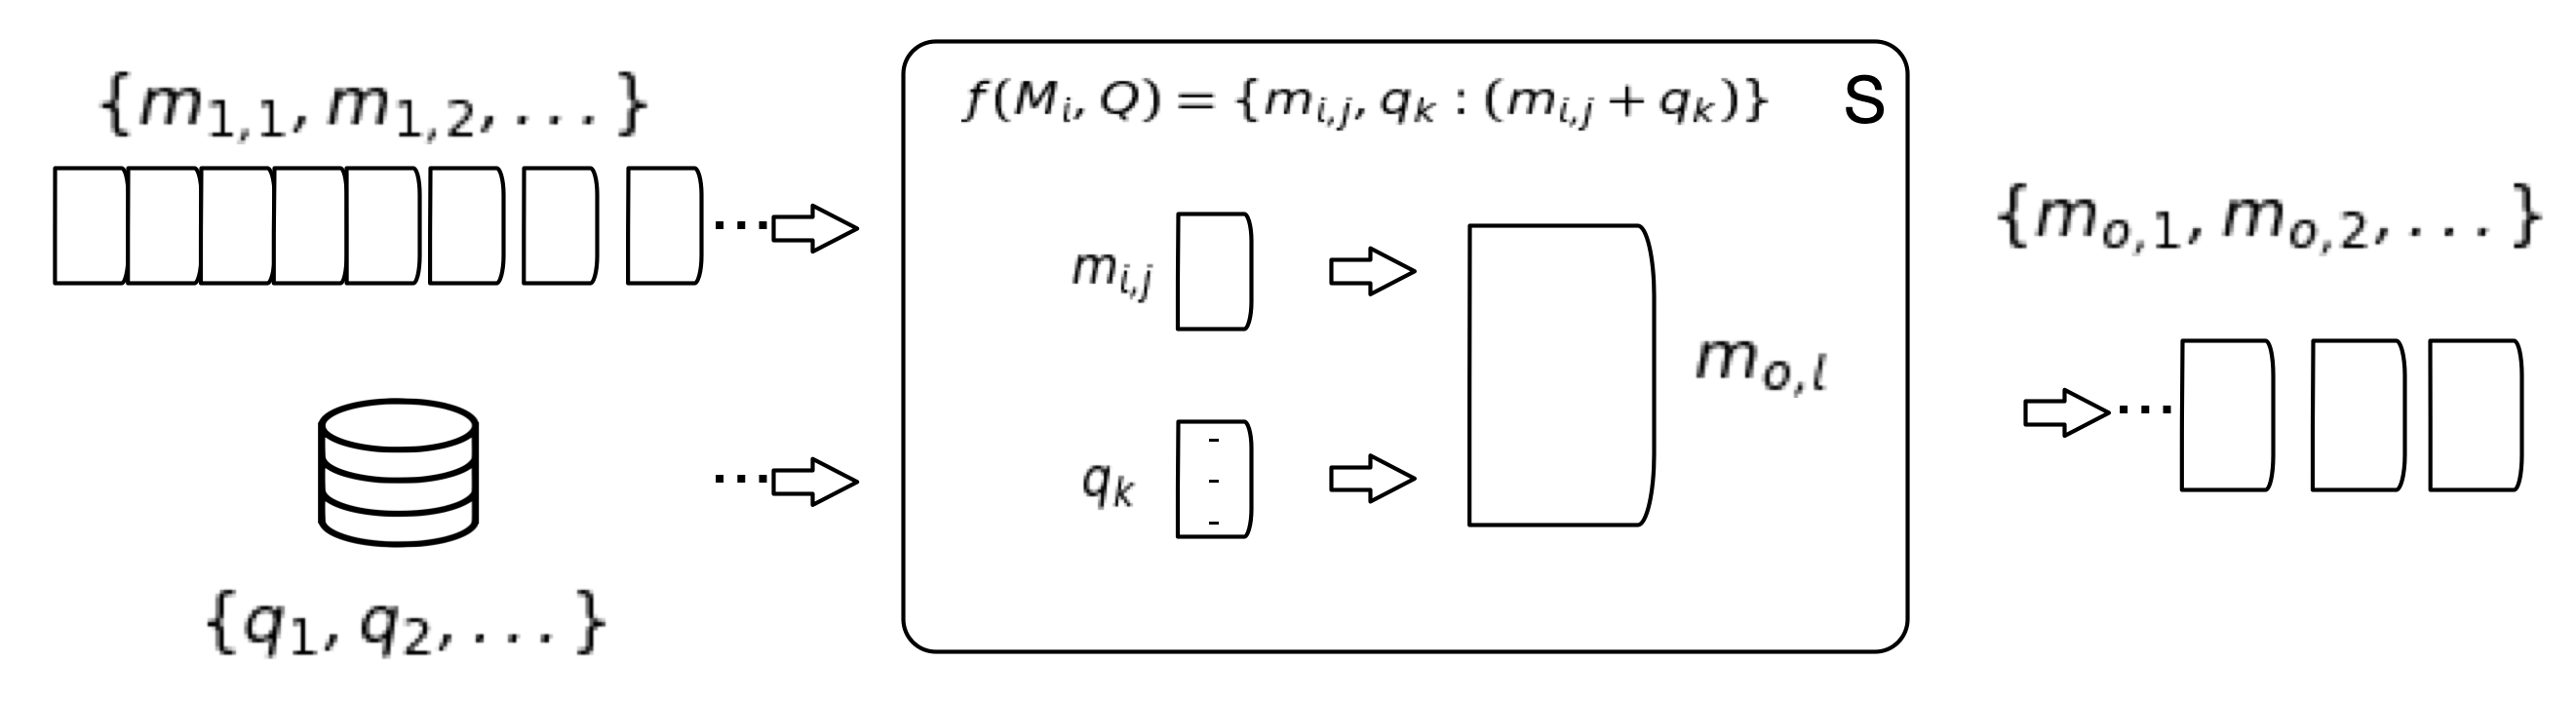
\includegraphics[scale=0.6]{stream_local_state_aggregator_function}
\centering
\caption {Service S aggregates $m_i$ with query results $q_i$ obtained from a local data store.}
\label{fig:stream_local_state_aggregator_function}
\end{figure}


\paragraph{Persistence Function} - Service $S$ observes messages $m_i$ and is responsible for persisting them to a data store where their contents can later be queried (see Figure \ref{fig:stream_persistence_function}). Although persistence of data to, and subsequent querying of data from, a store, such as a database, are comparatively more expensive operations than immediate reasoning over a live data stream, such mechanisms are necessary for situations where data may need to be accessed multiple times, or where data may need to be retained for audit purposes.

\begin{figure}[H]
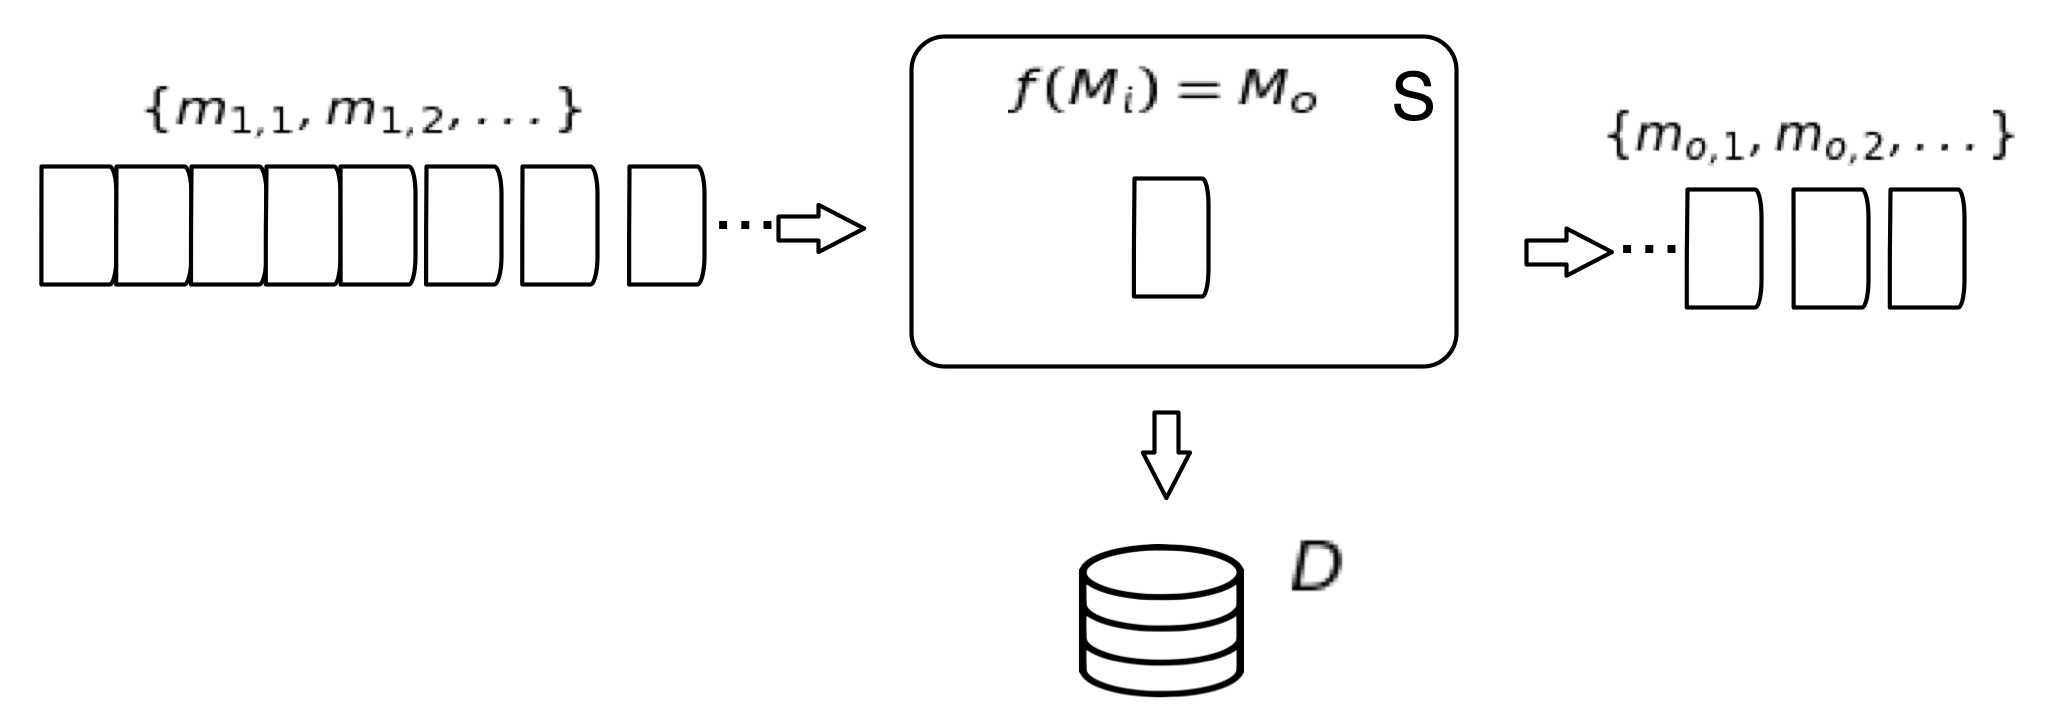
\includegraphics[scale=0.6]{stream_persistence_function}
\centering
\caption {Service $S$ processes messages $m_i$ into persistent storage. The output stream $M_o$ contains persistence confirmation and error events.}
\label{fig:stream_persistence_function}
\end{figure}

\paragraph{Query Function} - Service $S$ observes a stream of queries $Q_i$. The queries are fulfilled against a data store $D$ and the results emitted via the output stream $M_o$.

\begin{figure}[H]
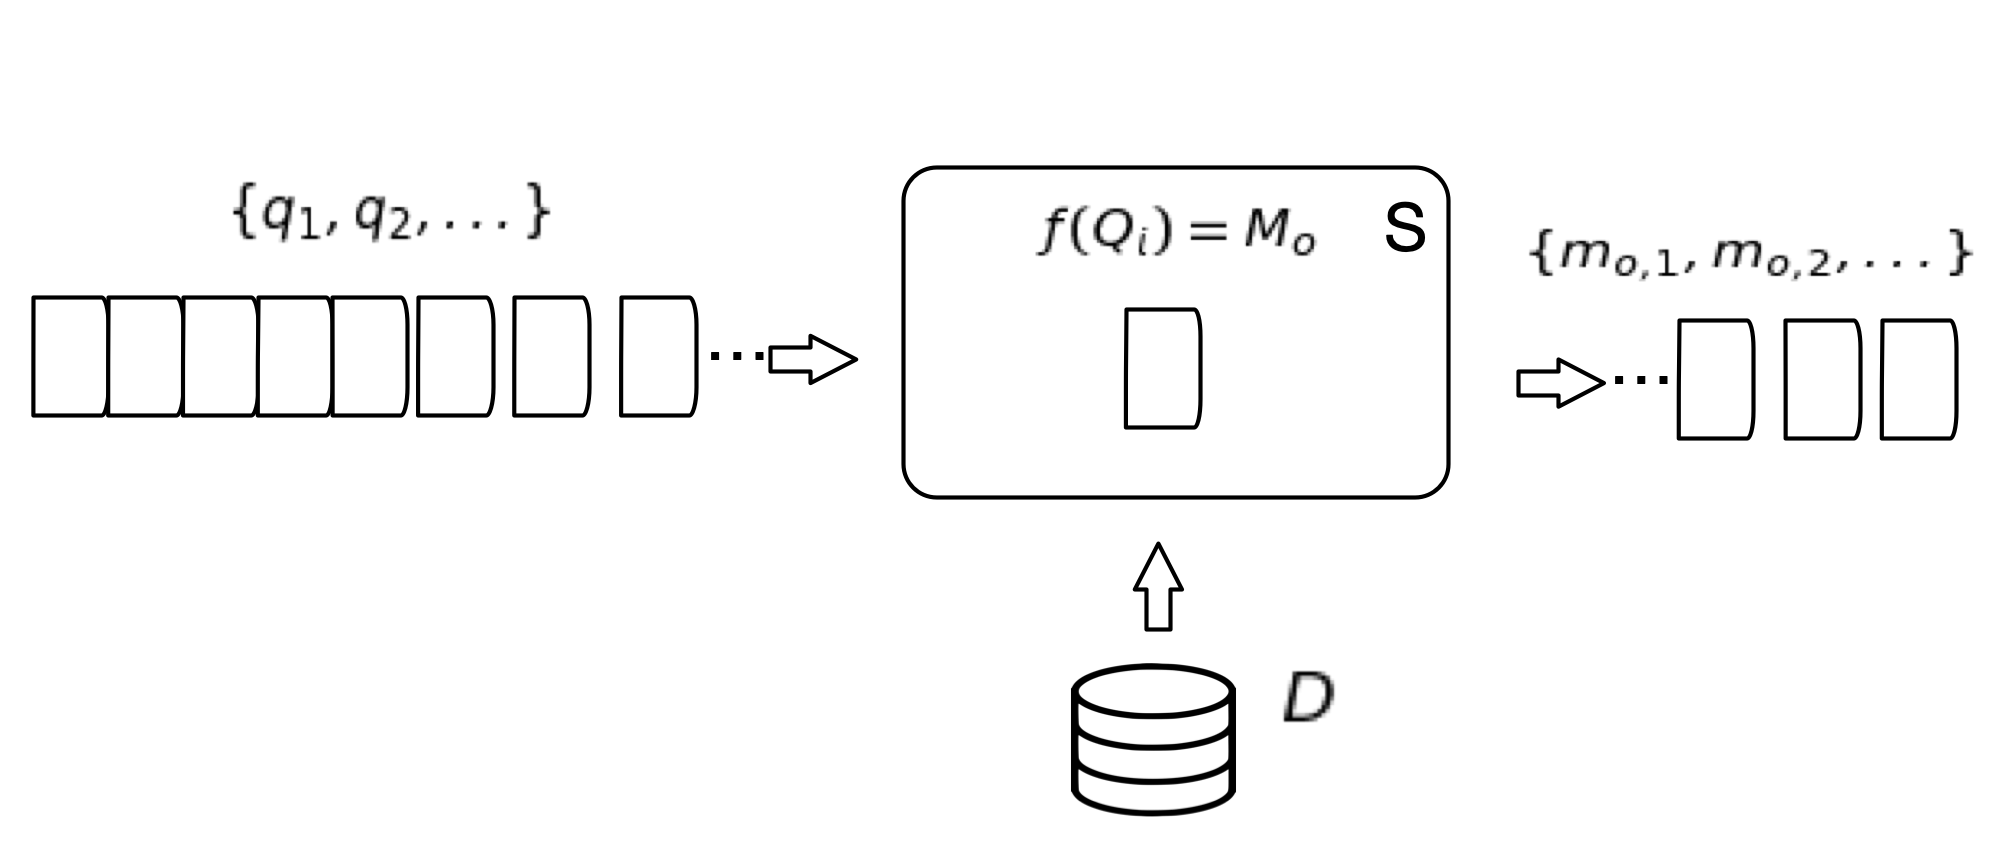
\includegraphics[scale=0.6]{stream_query_function}
\centering
\caption {Service S filters messages from input stream $M$ and only allows through those that pass the filtering condition.}
\label{fig:stream_query_function}
\end{figure}

The basic operations above can be combined to produce arbitrarily complex logic on data streams.

One of the key advantages of a service-oriented approach is that, because services are typically constantly executing, it naturally lends itself to an examination of the system's runtime characteristics. This applies to both service-internal characteristics that are related to each operation a service performs, as well as to external characteristics that relate to the contracts a service establishes with its dependencies. We consider both of these.

For each given operation $o_i \in S$ it is instrumental to understand the resource requirements of the operation on typical inputs and limiting factors that affect the efficiency with which the operation can be performed by $S$. Of particular interest are the per-operation profiles of:

\begin{itemize}
    \item CPU utilization
    \item RAM
    \item Secondary storage
    \item Network utilization
\end{itemize}

If $o_i$ is a long-running operation that takes multiple seconds to complete on average, a detailed distribution in time of each metric above may be necessary. If the operation can be completed at a sub-second rate then summary statistics (min, max, mean, median, inter-quartile range, 90th, and 99th percentiles) may be sufficient. This level of understanding is necessary in order to make sure that the service can adequately deal with the incoming message stream while the messages are first loaded into memory, since subsequent retrieval from secondary storage is several orders of magnitude slower and may cause further delays in processing. If $o_i$ is stateless, i.e. it does not require the storage and retrieval of any local state that depends on the content of each arriving message $m_j \in M_i$, then the service $S$ can be scaled "horizontally"\autocite{vaquero2011dynamically} with respect to $o_i$. Given that the performance-limiting condition of $o_i$ is known (CPU, memory, etc.), the ability of $S$ to efficiently deal with fluctuations in the rate of incoming messages $M_i$ can be successfully achieved simply by adding and removing servers that execute $S$ (see Figure \ref{fig:horizontal_vs_vertical_scaling}), which can be done automatically\autocite{mao2011auto}. If $o_i$ is stateful and requires access to databases, or predictable request routing via sessions, then horizontal scalability may not be possible and thus, detailed understanding of the performance profile and performance-limiting conditions of $o_i$ is even more important as vertical scaling of services is more expensive and challenging to accomplish, and may increase system complexity by necessitating data partitioning, for example\autocite{vaquero2011dynamically}.

\begin{figure}[H]
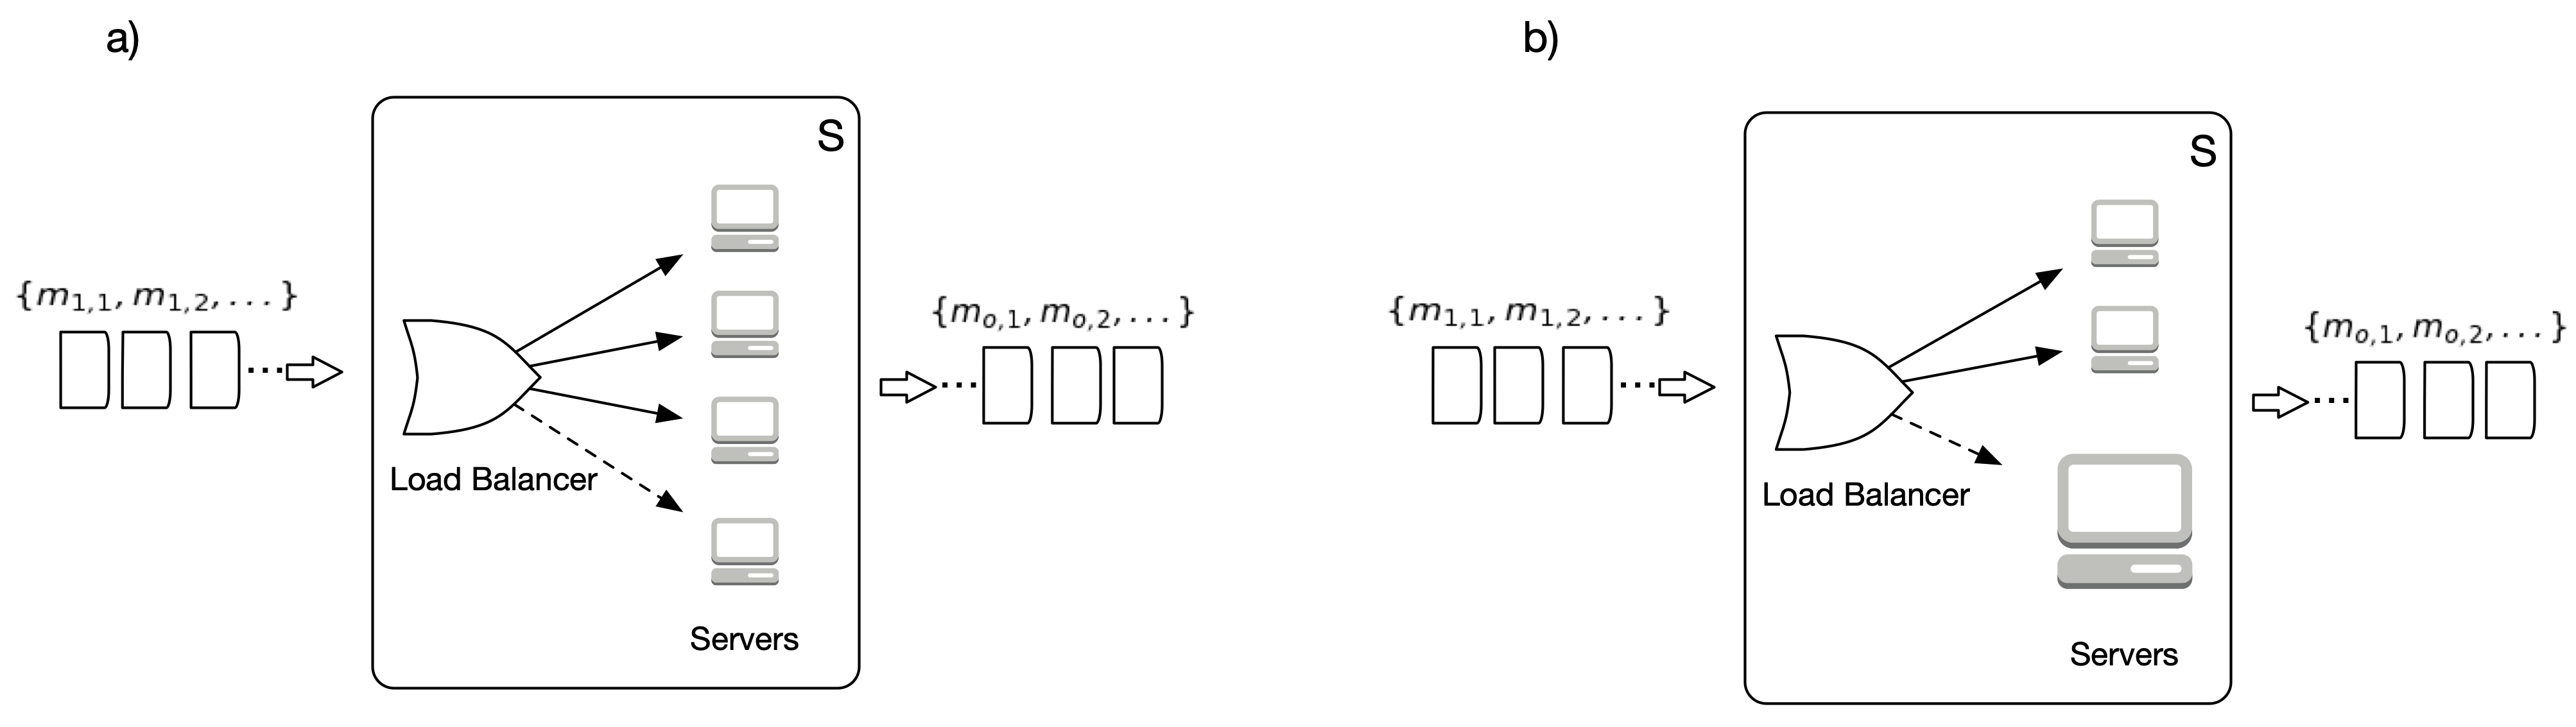
\includegraphics[scale=0.44]{horizontal_vs_vertical_scaling}
\centering
\caption {a) In horizontal scaling new servers are added and removed (dashed arrow) behind a load balancer as the rate of data stream $M_i$ fluctuates. b) In vertical scaling more powerful servers need to be launched (dashed arrow) to replace smaller servers (with potential service outage) when the rate of $M_i$ increases beyond capacity.}
\label{fig:horizontal_vs_vertical_scaling}
\end{figure}

Assume service $S$ implements operation $o$ supported by $n$ physical servers $V = \{v_j: j \in [1,n]\}$ by consuming a stream of incoming messages $M_i$. For a suitable time increment $t$, let $r_{M_i} = |M_i|/t$ be the incoming message arrival rate, and $r_{M_{o,j}} = |M_{o,j}|/t$ be the processing rate for server $v_j$. If $r_{M_i} > \sum_{j=1}^n r_{M_{o,j}}$, then $S$ will not be able to adequately process all of the incoming messages from $M_i$ and messages will either be lost or need to be backlogged while more servers are added to $S$ to deal with the incoming message rate. Since commissioning new servers takes considerable time and the timing and magnitude of increases in $r_{M_i}$ may be unpredictable, serious information loss may result if measures are not put in place to mitigate the message rate fluctuations. 

A queue is the mechanism that we put in place to address this concern (see Figure \ref{fig:queue}). A queue $Q$ is a message buffering system which consists of a set of $n$ "topics" $P = \{p_i: i \in [1,n]\}$, where each topic is a tuple of the form $p_i = (D_p,B_p,C_p)$. Here $D_p = \{d_i: i\in [1,k]\}$ is a set of $k$ data producers that put messages into $Q$, $B_p$ is a message buffer of max capacity $N_{max}$ dictated by underlying server hardware characteristics, containing a sequence of messages $\{m_t, m_{t-1},m_{t-2},....,m_1\}$ that are accessible in a Fist In First Out (FIFO) manner, and $C_p = \{c_i: i \in [1,l]\}$ is a set of $l$ consumers that are interested in observing messages from $p_i$.

\begin{figure}[H]
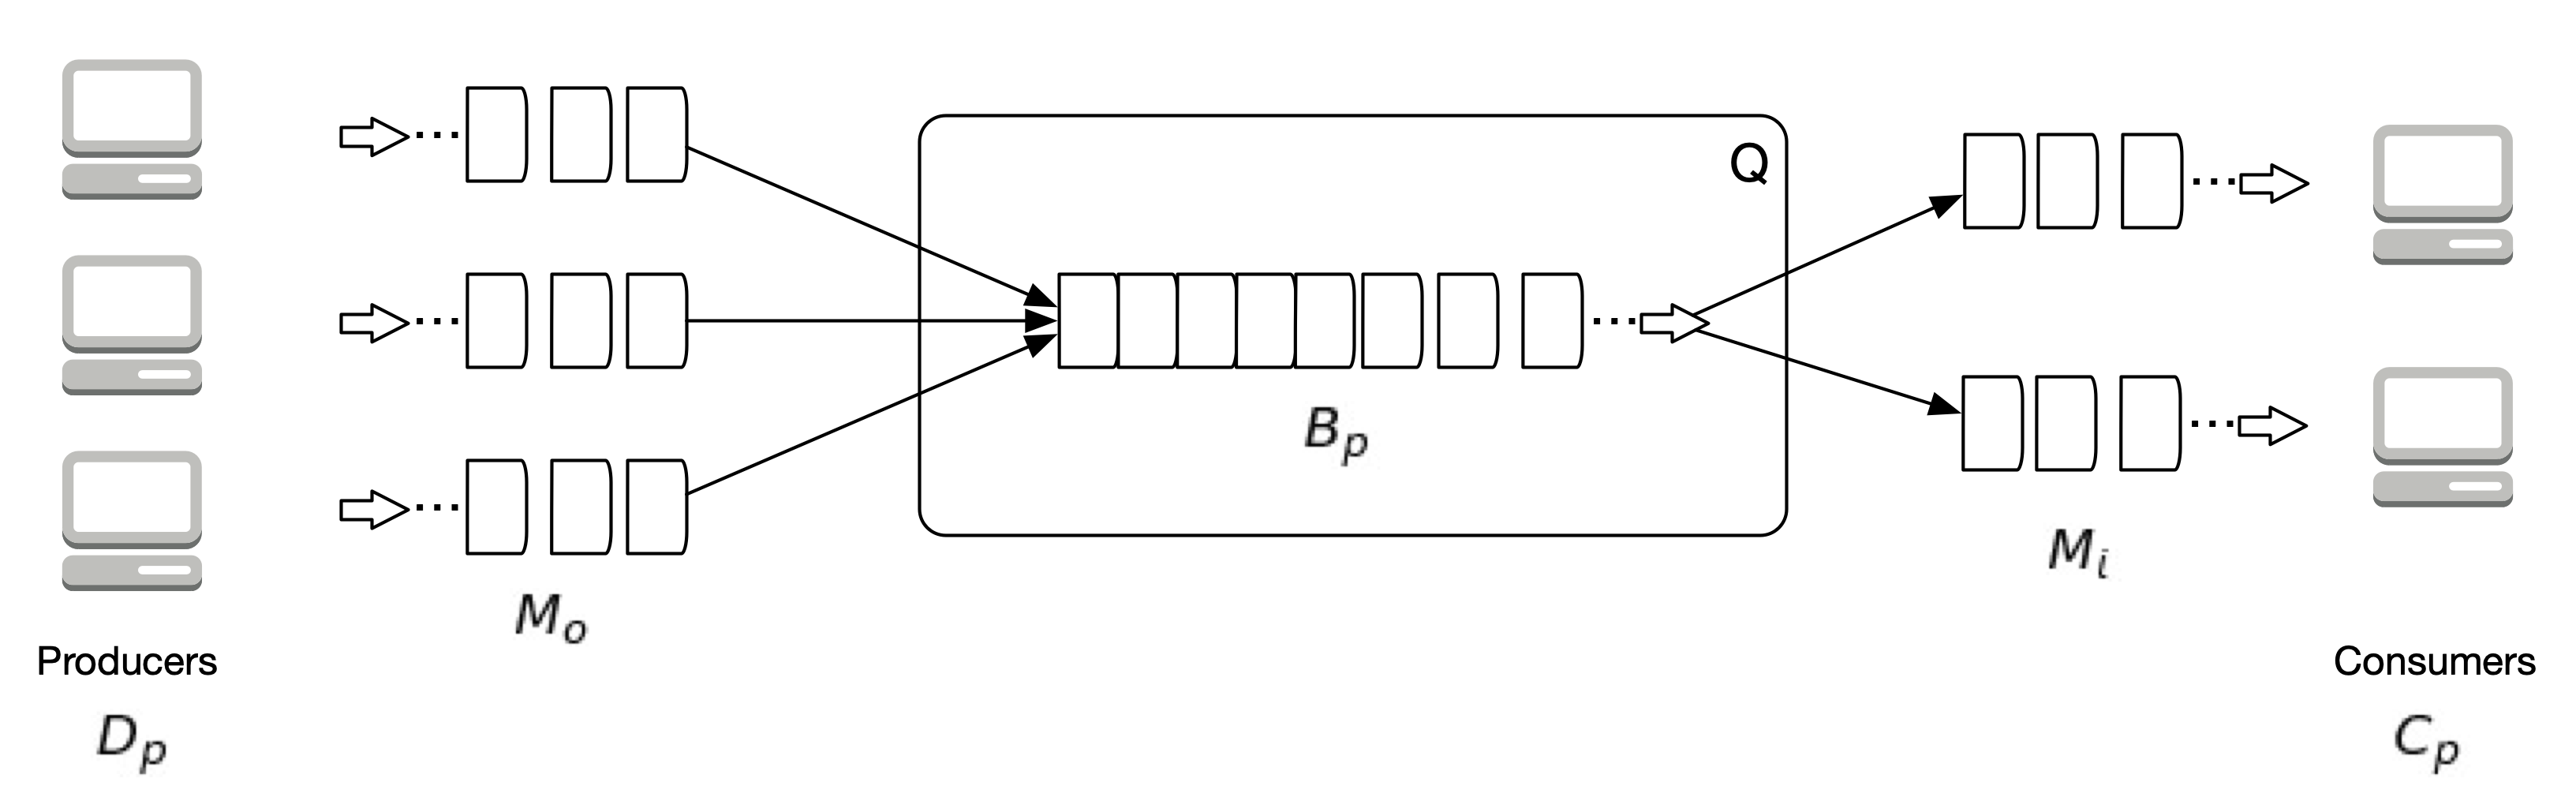
\includegraphics[scale=0.54]{queue}
\centering
\caption A queue $Q$ establishes a message buffer $B_p$ between a set of message producers $D_p$ and consumers $C_p$, for a given topic $p$.
\label{fig:queue}
\end{figure}

Messages arrive into a particular topic of $Q$ from all producers $D_p$, and are marked safe for deletion only when all of the subscribed consumers $C_p$ have observed a particular message. Thus, for topic $p_i$, the incoming message rate is $\displaystyle R_i = \sum_{j=1}^k r_{M_{o,j}}$ i.e. the sum of the message processing rates for all of the producers for this topic. The queue message processing rate $\displaystyle R_o = \min_{i \in [1,l]}\{r_{M_{o,i}}\}$ is the slowest message processing rate among all consumers. Assuming $R_i > R_o$ and that there are $N$ messages presently in $B_p$, there remains $t = \frac{N_{max} - N} {R_i - R_o}$ time before queue overflow occurs. The situation should then be remedied by allocating additional hardware to $Q$ or those services $S_i$ whose consumers are slowest, until the condition $R_o \ge R_i$ can be reliably maintained. If the queue does reach its maximum capacity overflow measures need to be put in place. Depending on the data stream in question data loss may or may not be acceptable. If data loss is acceptable then overflow messages can be simply discarded. If data loss is not acceptable then producers must block waiting for additional queue capacity to become available. This not only degrades performance locally, but can have a drastic effect on the entire system if the effects are allowed to percolate trough the complex distributed system. As message rates evolve through time with system load, the scheme above sets up a framework for flow control and hardware allocation within the architecture.

When designing a service-oriented system the interfaces of operations provided by the service are of utmost importance as they define the capabilities that the service offers to its clients. Of secondary, but also significant, importance is the set of Service-Level Agreements (SLAs)\autocite{wieder2011service} that a service advertises. These SLAs are a set of commitments that a service makes to its clients that describe the operational characteristics of the service, such as:

\begin{description}
    \item [Availability] - Guarantees related to the service uptime, maintenance outages, disaster recovery, etc.
    \item [Throughput] - The number of requests serviced per unit time.
    \item [Latency] - The delay between a request being sent and a response being received.
    \item [Abandonment Rate] - Proportion of requests that are never answered.
    \item [Error Rate] - Proportion of well-formed requests that result in an error.
\end{description}

Based on the SLAs that are advertised by a given service, the services that depend on it can make assumptions about expected runtime behavior, and take action when expectations are not met. Furthermore, when requirements evolve and features are added to or removed from a service, the impact on the advertised SLAs helps communicate the full effect of the changes. Lastly, the costs of operating a service are more clearly understood through the SLA framework, where improvements to a particular SLA metric, such as Transactions-Per-Minute (TPM) can be transparently traced to a corresponding increase in operational costs.

The set of services $\{S\}$ that communicate over data streams $\{M_{s,d}\}$, mediated by a set of queues $\{Q\}$ with a set of established SLAs $\{L_s\}$ together form the overall framework of Rheos that is used to tackle the challenges of large-scale genomic data processing in a manner the enables active tradeoffs between the competing constraints of cost, time, and accuracy. 

\section{Domain-specific Problems}\label{sec:main_body_domain_specific_problems}

Having laid out the general data-streaming service-oriented architecture of Rheos in the previous section we now turn to a discussion of the set of actual domain-specific problems that need to be solved within the data-streaming paradigm in order to enable the comprehensive genomic characterization of large cohorts of samples within Rheos, as we have set out to do. We make use of the flow of data types from the most raw to the most refined (see Figure \ref{fig:ngs_flow}) to illustrate the challenges that need to be solved during transformation of the input data between each successive stage, first in summary form, and then in full detail, below.

\begin{figure}[H]
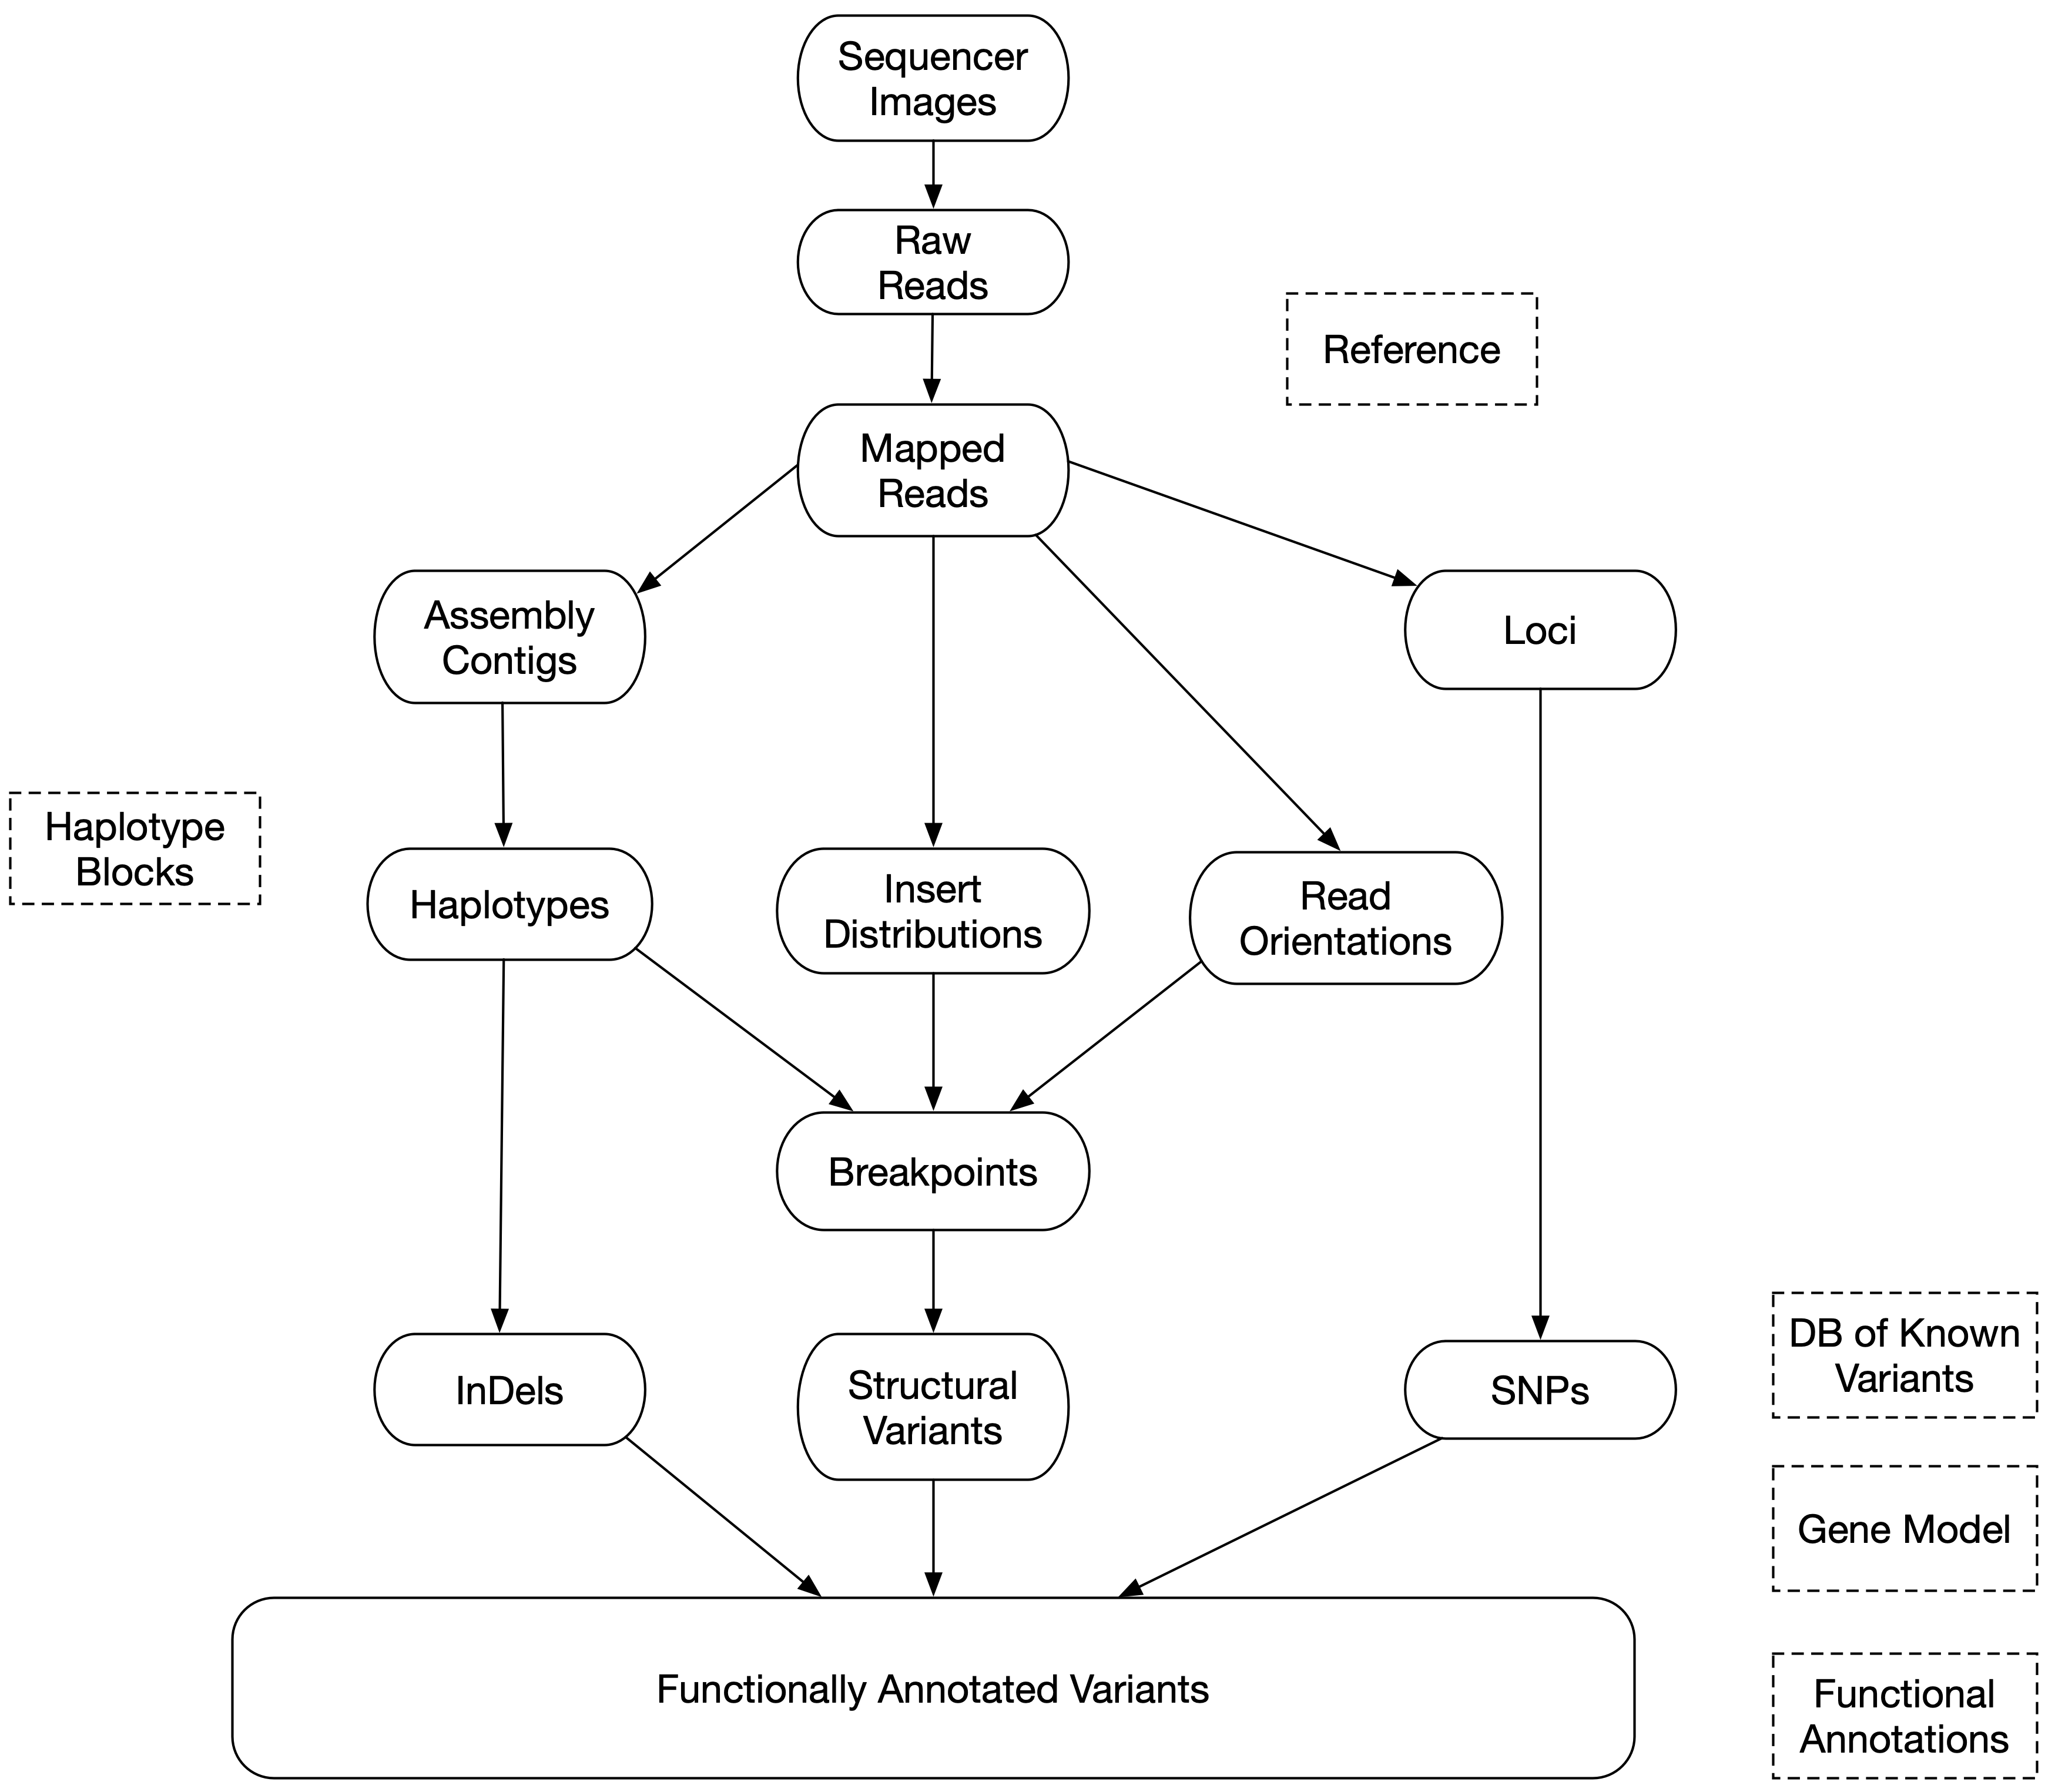
\includegraphics[scale=0.5]{ngs_flow}
\centering
\caption {The conceptual flow of data types within Rheos from the most raw - Sequencer Images, to the most refined - a set of Functionally Annotated Variants.}
\label{fig:ngs_flow}
\end{figure}
    
The most raw data type that is produced from a sequencing experiment is the set of raw image files generated by the sequencer. Although, conceptually, processing of the raw images could also be accomplished within Rheos, it is presently outside of the scope of this work. Instead, we assume the most basic data type to be raw sequencing reads, as found in a FASTQ\autocite{cock2009sanger} file. 

\begin{figure}[H]
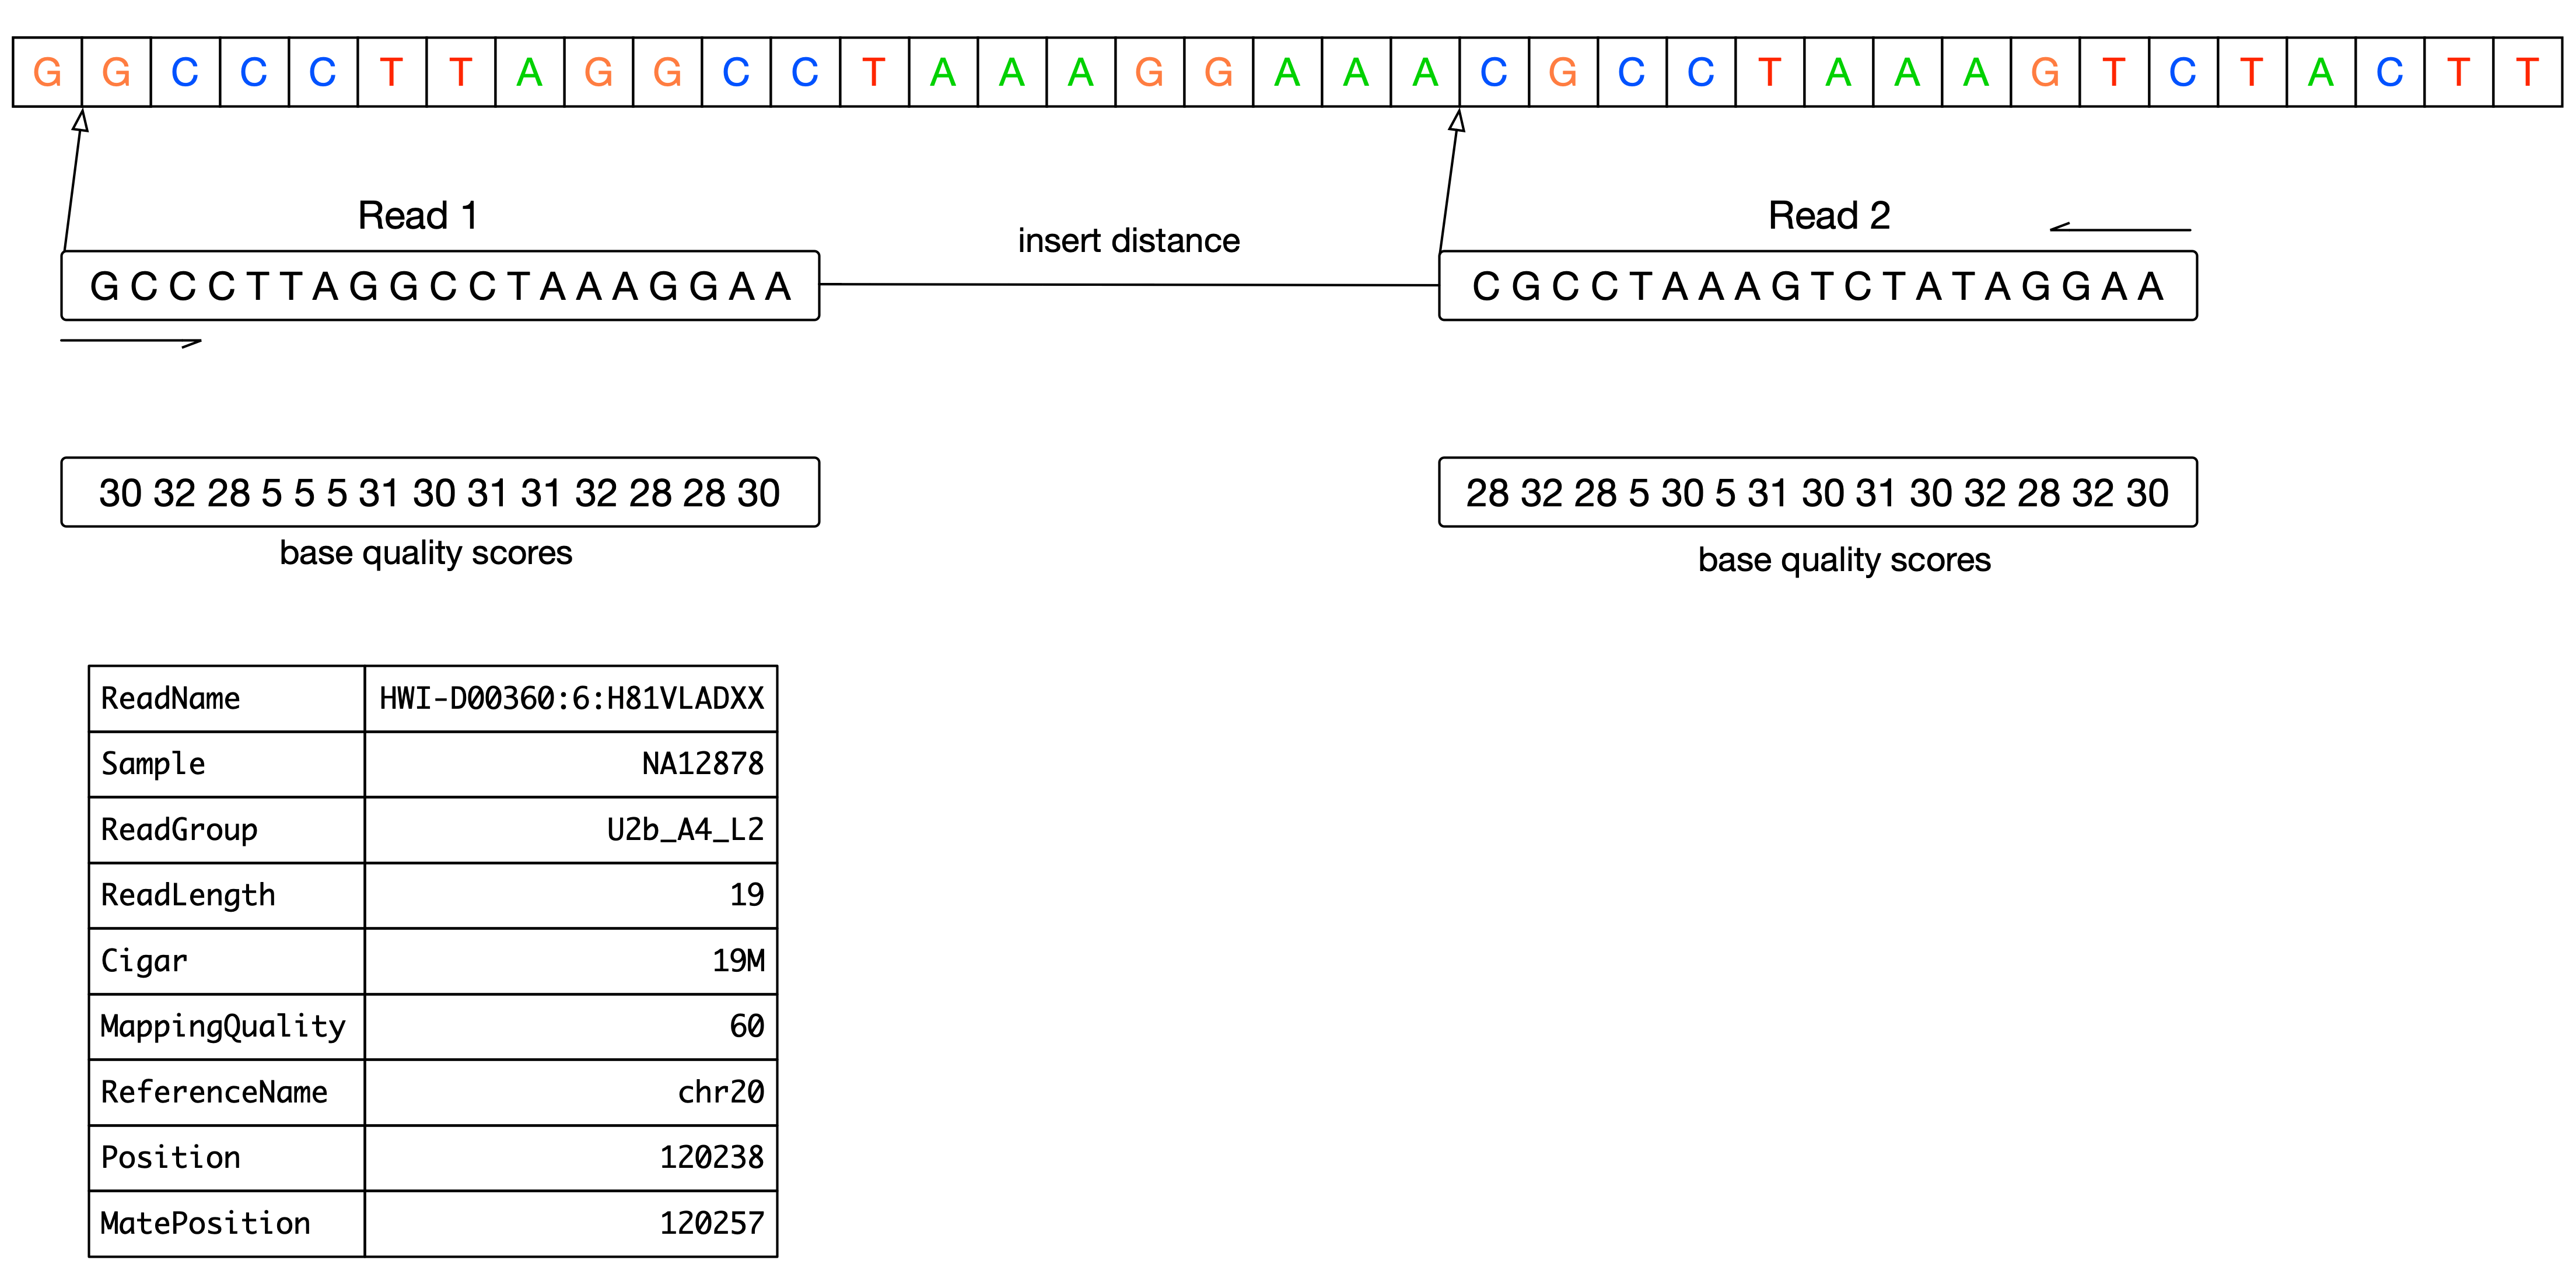
\includegraphics[scale=0.40]{read_pair}
\centering
\caption {A read-pair that is aligned to the reference.}
\label{fig:rheos_read_pair}
\end{figure}

Each read is a tuple of the form:

\begin{equation}
\label{eq:raw_read_message}
r = (s\_id, r\_id, b, q, f_p)
\end{equation}

where:

\begin{itemize}
    \item $s\_id$ - is the sample ID, which is unique among all samples.
    \item $r\_id$ - is the read ID, which is unique among all reads for that sample.
    \item $b = \{b_1, b_2,.....,b_n\}$ - is the sequence of DNA bases, where $b_i \in \{A,C,G,T,N\}$.
    \item $q = \{q_1, q_2,....,q_n\}$ - is the set of PHRED-scaled base quality scores corresponding to the probability that the base has been called incorrectly. See discussion on FASTQ format in Section \ref{sec:bg_file_formats} for details.
    \item $f_p \in \{True, False\}$ - is a boolean flag indicating whether this read is the first read in a pair.
\end{itemize}

\subsection{Read QC Metrics}
\label{sec:main_body_read_qc_metrics}

Section \ref{sec:bg_raw_data_qc} of the Background chapter discusses various metrics of interest that are based on observations of read data and the tools that are used to collect them. Here we describe how to collect the most typical metrics in the streaming paradigm of Rheos. As before, there are per-read metrics such as Base Quality Distribution, and Adapter Sequence Presence, as well as per-sample metrics such as Average GC Content, Insert Distribution, Read Length Distribution, and others. The utility of these metrics is to be able to set up filters for low quality data as well as input for downstream variant-calling models (see Section \ref{sec:bg_germline_sv_calling} for example). 

Assume that we are observing a stream $M_{raw} = \{m_i: m_i = (header, payload)\}$ of read messages where the payload is a read $r$ as defined above. Under the assumptions of Section \ref{sec:rheos_streaming_architecture} we know that the number of elements in the stream is unbounded. We are able to straightforwardly calculate incremental estimates for metrics such as mean, variance, max, and min, but require more sophisticated structures for computing estimates of rank statistics such as median and other quantiles to maintain operations in bounded space. We use the following update rules for min, max, mean, and variance\autocite{welford1962note} calculations:

\begin{equation}
    \label{eq:stream_min}
    min_k(M) =  \begin{cases}
        m_k,& \text{if } m_k < min_{k-1}(M)\\
        min_{k-1}(M),& \text{otherwise}
    \end{cases}
\end{equation}

\begin{equation}
    \label{eq:stream_max}
    max_k(M) =  \begin{cases}
        m_k,& \text{if } m_k > max_{k-1}(M)\\
        max_{k-1}(M),& \text{otherwise}
    \end{cases}
\end{equation}

\begin{equation}
    \label{eq:stream_mean}
    \mu_k(M) =  \mu_{k-1}(M) + \frac {m_k - \mu_{k-1}} {k} 
\end{equation}

\begin{equation}
    \label{eq:stream_variance}
    \sigma_k^2(M) =  \frac{\sigma_{k-1}^2(M) + (m_k - \mu_{k-1}(M))(m_k - \mu_k(M))}{k-1} 
\end{equation}

In order to set up the mechanisms to answer quantile queries the following definitions are used\autocite{garofalakis2016data}:

\begin{itemize}
    \item Given a set $S$ of size $n$, and a quantile $\phi \in [0,1]$, return $v \in S$ whose rank in sorted $S$ is $\phi n$. 
    \item An $\epsilon$-approximate $\phi$-quantile is a value $v$ whose rank $r*(v) \in [n(\phi-\epsilon), n(\phi+\epsilon)]$.
    \item A quantile summary is $Q = {q_1,q_2,....,q_l: q_1\le q_2 \le \dots \le q_l, q_i \in S, i \in [1,l]}$ where each $q_i$ has rank at least $rmin_Q(q_i)$ and at most $rmax_Q(q_i)$ in $S$, and $rmax_Q(q_1) \le \epsilon|S|$, and $rmin_Q(q_l) \ge (1-\epsilon)|S|$.
    \item A quantile summary $Q(\epsilon)$ is $\epsilon$-approximate if it can be used to answer any quantile query with $\epsilon$-accuracy.
\end{itemize}

We use two approaches for computing quantile summaries, one due to Greenwald and Khanna\autocite{greenwald2001space} is able to compute the quantile summary using $O(log(\epsilon n)/\epsilon)$ space, and the other by Shrivastava et al.\autocite{shrivastava2004medians} computes the quantile summary in $O(log(M)/\epsilon)$ when the values are integers in range $[1,M]$. Both algorithms work for a scenario where one node sees all of the data in a stream, but can also be generalized to topologies where the stream is observed by multiple nodes in parallel. 

We provide several examples of QC queries of interest that are specified on a data stream:

\paragraph{Average Base Quality} -  As an assessment of the individual quality of each read we are interested in the average base quality so that we can filter out reads that are of low quality as a whole. We use a Decorator Function construct from Section \ref{sec:rheos_data_streaming_model}. 

\bgroup
\def\arraystretch{1.5}
\begin{table}[!ht]
    \caption{Definition of $q_{av}$ which computes average base quality for a read}
    \label{tab:op_average_base_quality}
    {\begin{tabular}{l|p{12cm}}
    \toprule
    Inputs & \hangindent=1em$M_{raw} = \{m_i: m_i = (header, payload)\}$ where $m.payload = r = (s\_id, r\_id, b, q, f_p)$ as in \ref{eq:raw_read_message}.\\
    \cline{2-2}
    Operation & $q_{av} = \frac{\sum_{i \in [1,|r|]} r.q_i}{|r|}$\\
    \cline{2-2}
    {Outputs} & \hangindent=1em$M_{out} = \{m_i: m_i = (header, payload)\}$ where $m.payload = r = (s\_id, r\_id, b, q, f_p, q_{av})$\\
    \bottomrule
    \end{tabular}}
\end{table}
\egroup


\paragraph{Base Quality Distribution} - The distribution of base quality scores per base position of a read and per sample are of interest to investigate the presence of systemic biases in base quality scores as a function of the position within the read.

\begin{figure}[H]
    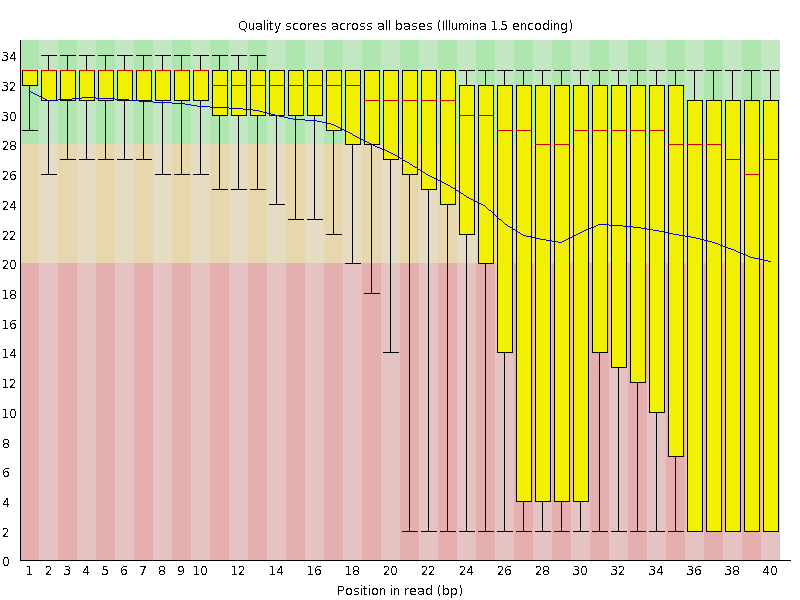
\includegraphics[scale=0.35]{fastqc_per_base_quality}
    \centering
    \caption {Distribution of base qualities per read position, from https://www.bioinformatics.babraham.ac.uk/projects/fastqc. Large quality drop-off can be see towards the end of the read.}
    \label{fig:main_body_fastqc_per_base_quality}
\end{figure} 

Because PHRED-scaled quality scores are integers that fall in a fixed range $q \in [0,96]$ building quantile summaries using the q-gram\autocite{shrivastava2004medians} approach is the most space-efficient. Because base quality scores need to be aggregated over many reads and tracked for many samples, a service that implements this functionality needs to keep local state, and the operation to update the quantile summaries based on incoming reads follows the Local State Aggregator pattern from Section \ref{sec:rheos_data_streaming_model}. 

\bgroup
\def\arraystretch{1.5}
\begin{table}[!ht]
    \caption{Definition of $updateQuantileSummaries()$}
    \label{tab:op_update_quantile_summaries}
    {\begin{tabular}{l|p{12cm}}
    \toprule
    Inputs & \hangindent=1em$M_{raw} = \{m_i: m_i = (header, payload)\}$ where $m.payload = r = (s\_id, r\_id, b, q, f_p)$ as in \ref{eq:raw_read_message}. \\
    \cline{2-2}
    Operation & $updateQuantileSummaries(r)$\\
    \cline{2-2}
    {Outputs} & \hangindent=1em$M_{out} = \{m_i: m_i = (header, payload)\}$ where $m.payload = (s\_id, Q_{bqd})$.\\
    \bottomrule
    \end{tabular}}
\end{table}
\egroup

Since the local state required for storing the quantile summaries may not fit in memory and may need to be persisted to disk, updating the summaries may be too expensive to do for every single read that is observed in a read input stream. Instead, reads may be buffered into a set of reservoirs, triggering an update of the quantile summaries when the reservoir is full. The contents of the reservoir would then be purged and an updated set of quantile summaries $Q_s,{bqg} = \{q_i: i\in [1,max\_bases]\}$, where each $q_i$ is a quantile summary corresponding to the Base Quality Distribution at a particular read position, issued to the output stream (see Algorithm \ref{ag:update_quantile_summaries_bqd}).

\begin{algorithm2e}[h]
\DontPrintSemicolon
\footnotesize
    \textbf{Function} {\sc updateBQDQuantileSummaries}$(r)$
    \Begin {
        $reservoir \gets ${\sc getReservoir$(r.s\_id)$}\;
        $reservoir.${\sc addNewRead$(r)$}\;
        \If {$reservoir.isFull$}{
            $summaries \gets ${\sc getQuantileSummaries$(r.s\_id)$}\;
            \For{$read$ {\bf in} $reservoir$}{
                \For{$index,read.q$ {\bf in} $read$}{
                    {\sc updateQGram$(summaries[index], read.q)$} \tcp*{per \autocite{shrivastava2004medians}}\;
                }
            }
            {\sc purgeReservoir$(reservoir)$}\;
            {\sc outputQuantileSummary$(r.s\_id, summaries)$}\;
        }
    } 
\caption{Updating quantile summaries for Base Quality Distribution.}
\label{ag:update_quantile_summaries_bqd}
\end{algorithm2e}

\paragraph{Insert Size Distribution} - The insert size distribution is an important metric because it is not only indicative of the overall quality of a sample's data, but it is also used by structural variant calling to find read-pairs that map abnormally far apart (indicating a deletion), or abnormally close together (indicating an insertion). 

\begin{figure}[H]
    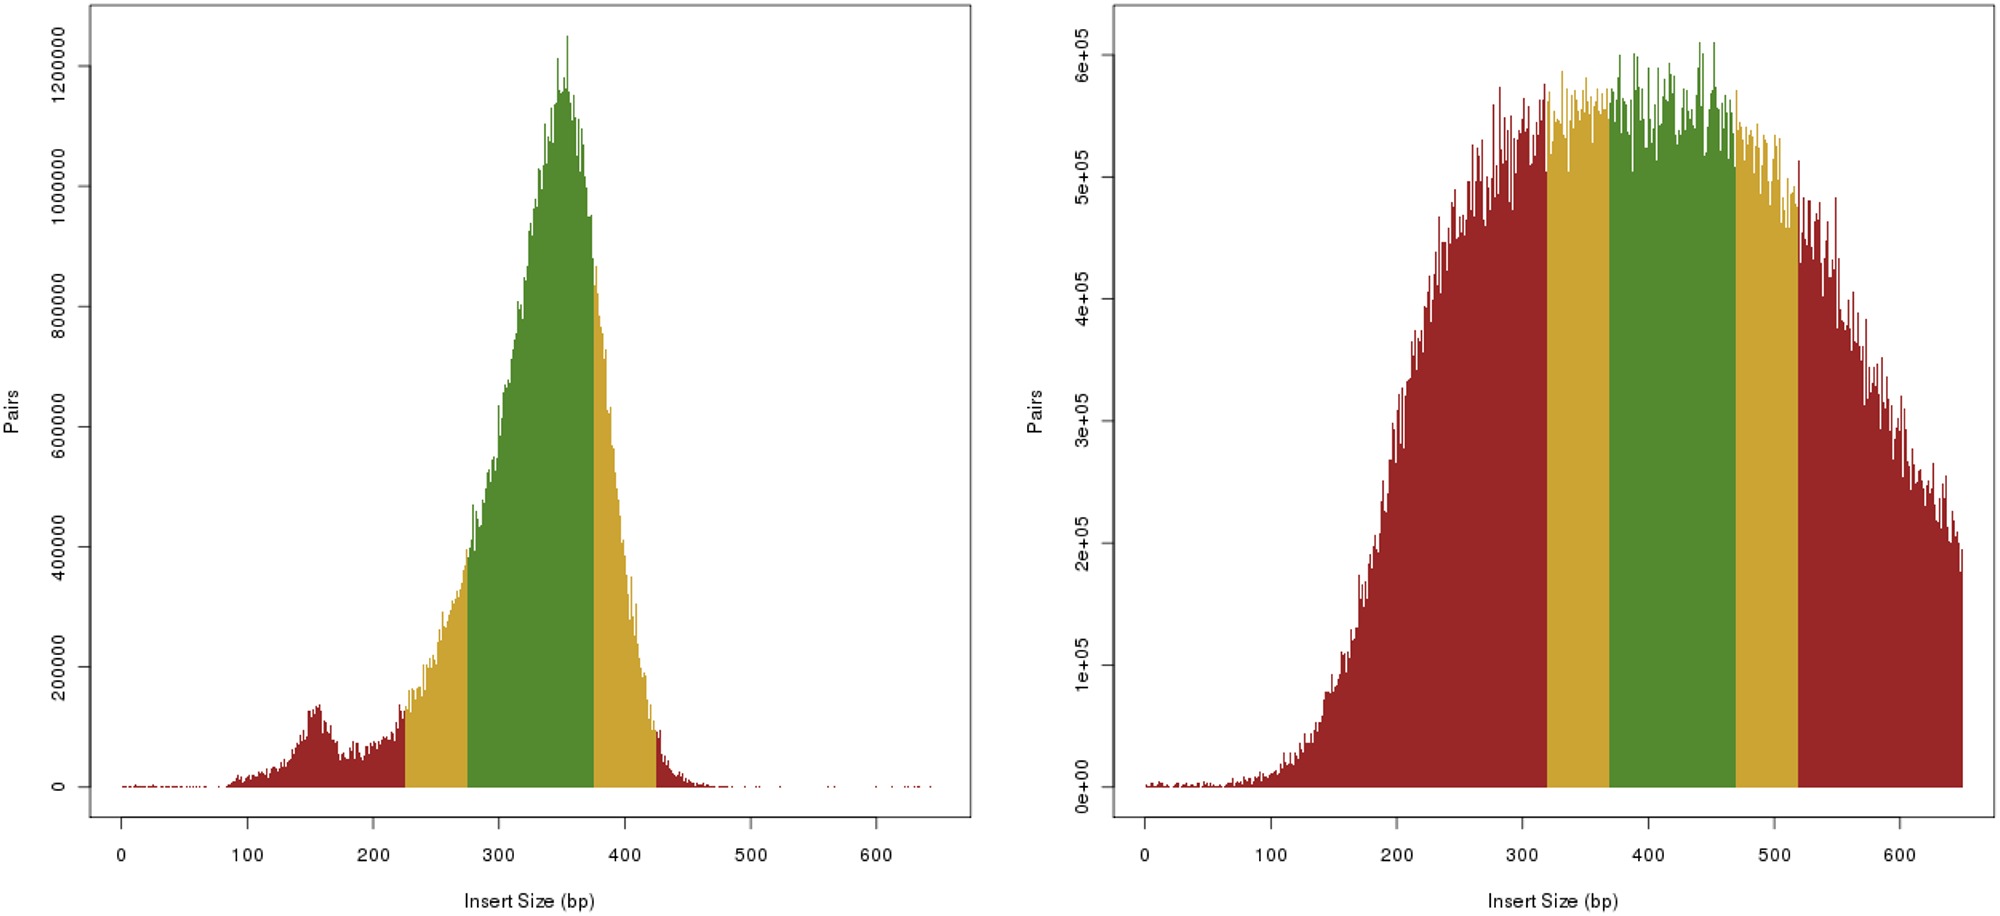
\includegraphics[scale=0.85]{insert_size_distribution}
    \centering
    \caption {Distribution of insert sizes from two ICGC pancreatic cancer patients DO35138 and DO22154.\autocite{stephens2016simulating}}
    \label{fig:insert_size_distribution}
\end{figure} 

Calculating this metric requires a stream of read-pairs, where both reads have been successfully mapped to the reference genome. Given a mapped read-pair $(r_1,r_2)$ where each read has a beginning coordinate $r.pos$ and an end coordinate $r.end$, the insert size is $l = r_2.end - r_1.pos$. We are interested in the mean, variance and quantiles of the insert size distribution. Because the insert length can be any size the quantile summary method of Greenwald and Khanna\autocite{greenwald2001space} is most appropriate for the quantiles. Read pairs are observed on the input stream and buffered in per-sample reservoirs. When a reservoir is full the read pairs are used to update and output an appropriate insert size distribution mean, variance, and quantile summary.

\bgroup
\def\arraystretch{1.5}
\begin{table}[!ht]
    \caption{Definition of $updateInsertSizeDistribution()$}
    \label{tab:op_update_insert_size_dist}
    {\begin{tabular}{l|p{12cm}}
    \toprule
    Inputs & \hangindent=1em$M_{pair} = \{m_i: m_i = (header, payload)\}$ where $m.payload = (r_1,r_2)$, and $r = (s\_id, r\_id, b, q, f_p)$ as in \ref{eq:raw_read_message}. \\
    \cline{2-2}
    Operation & $updateInsertSizeDistribution(s\_id,r_1, r_2)$\\
    \cline{2-2}
    {Outputs} & \hangindent=1em$M_{out} = \{m_i: m_i = (header, payload)\}$ where $m.payload = (s\_id, \mu_{isd}, \sigma_{isd}^2, Q_{isd})$.\\
    \bottomrule
    \end{tabular}}
\end{table}
\egroup

\begin{algorithm2e}[h]
    \DontPrintSemicolon
    \footnotesize
    \textbf{Function} {\sc updateInsertSizeDistribution}$(s\_id, r_1,r_2)$
    \Begin {
        $pairReservoir \gets ${\sc getReservoir$(s\_id)$}\;
        $pairReservoir.${\sc addNewReadPair$(r_1, r_2)$}\;
        \If {$pairReservoir.isFull$}{
            $summary \gets ${\sc getQuantileSummary$(s\_id)$}\;
            $mu \gets ${\sc getMu$(s\_id)$}\;
            $sigmaSq \gets ${\sc getSigmaSq$(s\_id)$}\;
            \For{($r_1, r_2$) {\bf in }$pairReservoir$}{
                $insertSize$ \gets $r_2.end - r_1.pos$\;
                {\sc updateQuantileSummary$(summary, insertSize)$} \tcc*{per \autocite{greenwald2001space}}\;
                $newMu$ \gets {\sc updateMu$(mu, insertSize)$} \tcc*{using Eq. \ref{eq:stream_mean}}\;
                $newSigmaSq$ \gets {\sc updateSigmaSQ$(sigmaSq, mu, newMu, insertSize)$} \tcc*{using Eq. \ref{eq:stream_variance}}\;
            }
            {\sc purgeReservoir$(pairReservoir)$}\;
            {\sc outputInsertSizeDistribution$(s\_id, newMu, newSigmaSq, summary)$}\;
        }
    }
    \caption{Updating metrics for Insert Size Distribution.}\label{ag:update_metrics_isd}
\end{algorithm2e}

Other QC metrics, such as those measuring GC Content Distribution, Read Length Distribution, etc. can be collected analogously. 

\subsection{Alignment}\label{sec:main_body_alignment}

Section \ref{sec:bg_alignment} of Chapter \ref{ch:background} provides an overview of the existing approaches in the extremely important and computationally intensive genome alignment stage of the overall NGS processing pipeline. In the overall data flow diagram (Figure \ref{fig:ngs_flow}), alignment is primarily responsible for transforming Raw Reads into Mapped Reads, but is also used in QC (insert size distribution, sample contamination) as well as in the construction and evaluation of local haplotypes for variant calling. In this section we describe the adaptation of already established read mapping best practices to the stream and services based domain of Rheos. Because of the generally independent nature of individual read observations (except for read pairs), this read mapping problem is highly amenable to a stream-based approach. We begin by enumerating and describing the types of alignment tasks that the Rheos framework needs to be able to accomplish and follow up by describing how these tasks will be performed within Rheos.

\begin{description}
    \item [Single read alignment to reference] - Given a representation of the human reference genome we are interested in finding a coordinate relative to this reference where the given read best matches. If we are not able to find a high quality mapping the read should be flagged as unmapped.
    \item [Read pair alignment to reference] - Given a pair of reads and an estimate of fragment size, attempt to find a high quality consistent mapping for both reads in a window around the expected fragment size.
    \item [Single read alignment to multiple references] - Given a read and a database of several genome references from multiple species determine if the read has a high quality mapping in any of the references. This can be used for assessing sample contamination.
    \item [Candidate haplotype alignment to reference] - Given a candidate haplotype i.e. a contiguous (potentially long) sequence locally assembled from a set of reads, align the sequence to the reference genome to identify locations of potential variation.
    \item [Single read split-alignment to reference] - Given a read that does not align well to a contiguous region of the reference, search for an alignment where individual pieces of the read might align to separate and possibly distant locations on the reference, suggesting that the read spans a region of structural variation.
\end{description}

\paragraph{Single read alignment to reference} 
Assume we are observing a data stream of raw unmapped short (<500 bp) reads $M_{raw} = \{m_i: m_i = (header, payload)\}$ where $m.payload = r = (s\_id, r\_id, b, q, f_p)$ as in \ref{eq:raw_read_message}. Using an existing human reference genome, such as \emph{GRCh38}, we would like to align each read in $m.payload$ to produce two new output streams $M_{aln}$ and $M_{unaln}$, depending on alignment results. $M_{aln}$, will contain messages from $M_{raw}$ with additional attributes related to the alignment, as described in Section \ref{sec:bg_sam_bam}, replicating the information contained in a SAM alignment record (see Table \ref{tab:sam_file_body_mandatory_fields}). $M_{unaln}$ shall contain reads from $M_{raw}$ that failed to align to a reference sequence, with an additional flag $unmapped=true$.

For $M_{aln}$ the following values are computed:

\begin{description}
    \item [rname] - name of the reference contig read is aligned to.
    \item [pos] - 1-based position offset of the left end of the read alignment to the contig specified in qname.
    \item [mapq] - Phred-scaled mapping quality representing probability that the read is misaligned.
    \item [cigar] - CIGAR string (as in SAM specification Section \ref{sec:bg_sam_bam}).
    \item [flags] - a tuple of flags as specified in the FLAG field of a SAM record.
\end{description}

Given that BWT and FM-index based algorithms\autocite{langmead2012fast},\autocite{Li2013} have currently shown the best balanced performance characteristics on both simulated and real data (see Figures \ref{fig:bwa_mem_comparison}, \ref{fig:bowtie_2_performance}) and the fact that these algorithms are amenable to straightforward parallelization, as in \autocite{langmead2009searching} for example, we adopt this approach as well in Rheos. Using this approach we will be able to locate $k$ locations for potential matches of a seed $d_i$ of read sequence $r.q$ in $\mathcal{O}(|r.q.d_i| + k)$ time using a data structure that takes $\mathcal{O}(|R|)$ space for a reference genome $R$. The seeds will then be extended using a version of Smith-Waterman\autocite{smith1981comparison} dynamic programming based alignment with affine gap penalites that can be performed in $\mathcal{O}(|R||r.q|)$ time and $\mathcal{O}(|r.q|)$ space based on \autocite{myers1988optimal} and \autocite{farrar2006striped}. The overall processing pipeline closely follows Figure \ref{fig:bowtie_pipeline} i.e. given a read $r$: 

\begin{itemize}
    \item Using Algorithm \ref{alg:find_smems} find a set $E$ of SMEMs of $r.q$\autocite{Li2013} using the FMD index formulation described in Section \ref{sec:bg_alignment} in relation to BWA. 
    \item Organize SMEMs $e_i$ in $E$ into co-linear chains of the form $C_i = \{(e_j,e_{j+1},p)\}$, where $e_j$ and $e_{j+1}$ are neighbouring SMEMs in the chain and $p$ is the mapping coordinate of $e_j$. Here co-linearity means that the SMEMs are in the same order and orientation on the query read and the reference genome, and a chain of maximal length is selected at each genomic location for the following processing step.
    \item For each chain, complete the read alignment between chain seeds using a vectorized SIMD-enabled implementation of Smith-Waterman local alignment, as in \autocite{farrar2006striped}.
    \item Output alignment with the highest alignment score (based on number of mismatched bases and number of secondary alignments) if it's above a minimum quality threshold. 
\end{itemize}

Because of the FMD index formulation used in finding seeds, both the read and its complement are considered at the same time. $rname$ and $pos$ values are straightforwardly obtained from the coordinate and name of the leftmost position of the winning alignment. The $cigar$ string (see Figure \ref{fig:main_body_cigar_string}) is produced directly as a concatenation of the winning dynamic programming paths, and the SMEM seeds which are exact matches. $mapq$ converts alignment score to Phred-scale, and $flags$ encode a set of boolean values as per the SAM spec. This provides all of the information necessary for the output mapping.

\begin{figure}[H]
    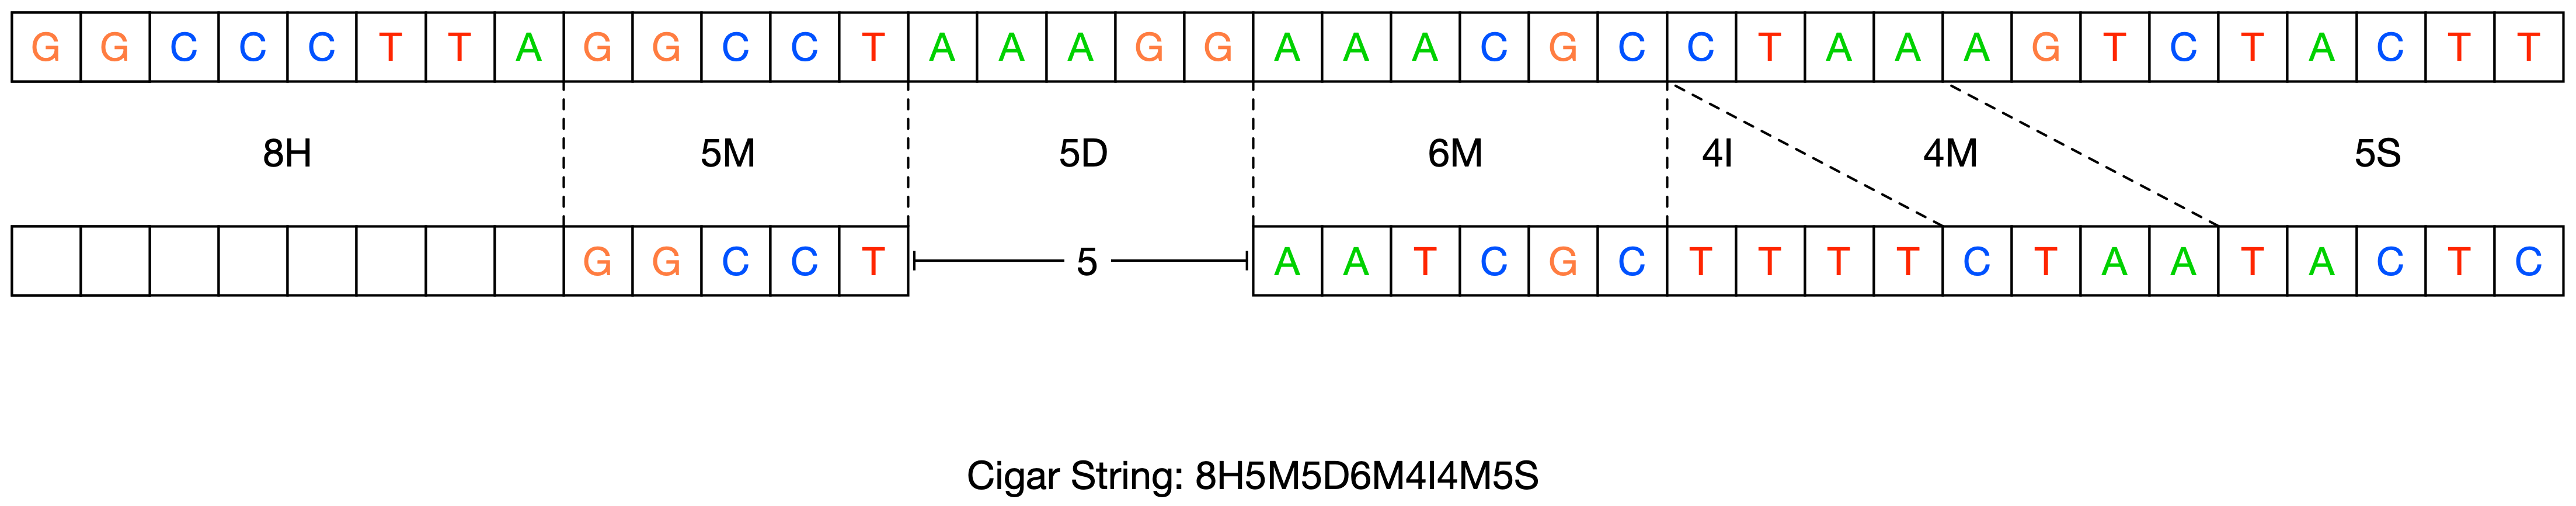
\includegraphics[scale=0.40]{cigar_string}
    \centering
    \caption {Example of an alignment CIGAR string.}
    \label{fig:main_body_cigar_string}
\end{figure}

If a co-linear set of seeds is not available, or the alignment score fails to reach the predetermined minimal score threshold then the read is emitted into the unmapped read stream with an appropriate flag set.

\bgroup
\def\arraystretch{1.5}
\begin{table}[!ht]
    \caption{Definition of $mapToReference()$}
    \label{tab:op_map_read_to_reference}
    {\begin{tabular}{l|p{12cm}}
    \toprule
    Inputs & \hangindent=1em$M_{raw} = \{m_i: m_i = (header, payload)\}$ where $m.payload = r = (s\_id, r\_id, b, q, f_p)$ as in \ref{eq:raw_read_message}. \\
    \cline{2-2}
    Operation & $mapToReference(r, ref\_id)$\\
    \cline{2-2}
    \multirow{2}{*}{Outputs} & \hangindent=1em$M_{aln} = \{m_i: m_i = (header, r)\} \text{ where } r = (s\_id, ref\_id, r\_id, b, q, f_p, rname, pos, mapq, cigar, flags)$\\
    & \hangindent=1em $M_{unaln} = \{m_i: m_i = (header, r)\} \text{  where } r = (s\_id, r\_id, b, q, f_p, unmapped=true)$\\
    \bottomrule
    \end{tabular}}
\end{table}
\egroup

The reference pointed to by $ref_id$ when $mapToReference()$ is invoked consists of the typical data structures required by the FM Index i.e. the reference BWT, suffix array, occurrence array, as in \autocite{ferragina2000opportunistic}, but encoding both the forward and reverse complement of the reference sequence as in \autocite{Li2013} to produce the FMD index. Because the reference sequence is static, updated less frequently than once a year, the requisite data structures can be computed once offline and stored in secondary storage. During service initialization they are loaded in RAM and kept memory-resident for the duration of the operation of the service. Because, once computed, the reference index is read-only it can be accessed in a thread-safe manner by multiple concurrent threads without the need for explicit concurrency management. Because of the embarrassingly-parallel nature of read alignment this operation can be scaled up as necessary simply by adding servers, provided additional computational resources exist, and network capacity is not exhausted.

\paragraph{Read pair alignment to reference} 
Since paired-end sequencing produces two reads that represent the opposite ends of a single molecule of approximately known size (known as insert size) it is possible to use knowledge about the insert size distribution along with corresponding pairs of reads to improve the quality of mapping for these reads, and even rescue mappings for reads that do not have a high quality unique mapping themselves but are anchored by a high quality mate. The mapping operation in this context proceeds similarly to the already described single read mapping but requires an input stream of read pairs along with a stream of sample QC metrics, including the empirical insert size distribution (as described in Section \ref{sec:main_body_read_qc_metrics}).

Depending on the result of the mapping operation for each read in a pair the output stream will contain pairs of reads of type \\
$r_{aln} = (s\_id, r\_id, b, q, f_p, rname, pos, mapq, cigar, flags)$\\
or \\
$r_{unaln} = (s\_id, r\_id, b, q, f_p, unmapped=true)$. 

\bgroup
\def\arraystretch{1.5}
\begin{table}[!ht]
    \caption{Definition of $mapPairToReference()$}
    \label{tab:op_map_pair_to_reference}
    {\begin{tabular}{l|p{12cm}}
    \toprule
    \multirow{2}{*}{Inputs} & \hangindent=1em$M_{pair} = \{m_i: m_i = (header, payload)\}$ where $m.payload = (r_1,r_2)$, and $r_i = (s\_id, r\_id, b, q, f_p)$ as in \ref{eq:raw_read_message}. \\
    & \hangindent=1em$M_{qc} = \{m_i: m_i = (header, payload)\}$ where $m.payload = (s\_id, \mu_{isd}, \sigma_{isd}^2, Q_{isd})$\\
    \cline{2-2}
    \multirow{2}{*}{Operations} & $mapPairToReference(r_1,r_2, ref\_id)$\\
    & $updateInsertSizeDistribution(s\_id,\mu_{isd}, \sigma_{isd}^2)$\\
    \cline{2-2}
    \multirow{2}{*}{Outputs} & \hangindent=1em$M_{aln} = \{m_i: m_i = (header, payload)\}$ where $m.payload = (r_1,r_2)$ and each read is of type $r_{aln}$\\
    & \hangindent=1em$M_{unaln} = \{m_i: m_i = (header, payload)\}$ where $m.payload = (r_1,r_2)$ and each read is of type $r_{aln}$ or $r_{unaln}$ depending on the outcome of mapping.\\
    \bottomrule
    \end{tabular}}
\end{table}
\egroup

In order to perform the $mapPairToReference()$ operation the service needs to have information about the insert size distribution for the sample the read pairs are originating from. It is notified with updated information about the insert size distribution by the $updateInsertSizeDistribution()$ operation which is subscribed to the appropriate message stream from the Read QC Service. This information is stored locally for each sample and may be cached. Assuming that the insert size distribution is approximately gaussian with mean $\mu_{isd}$ and variance $\sigma_{isd}^2$, which is the case for well-behaved samples, a scoring metric can be constructed that favours paired alignments that fall close to the expected insert size. This metric helps select among non-uniquely mapping reads. For instance, BWA-MEM uses the following metric:

\begin{equation}
    S_{ij}=S_i + S_j - \min{-a\log_4P(d_{ij}),U}
\end{equation}

Here $S_i$ and $S_j$ are the alignment scores for the individual reads in the pair obtained by single-end mapping via $mapToReference(r, ref\_id)$. $d_ij$ is the insert size implied by the mapping, $P(d_{i,j})$ is the probability of observing an insert size larger than $d$ under the assumption $D \sim \mathcal{N}(\mu_{isd}, \sigma_{isd}^2)$, $a$ is a matching score, and $U$ is a thresholding constant. Thus, given a set of possible mapping locations for each read in a pair, the joint mapping that maximizes the pairing metric is chosen.

$mapPairToReference()$ outputs read pairs to two output streams. If both reads are mapped successfully then they are output to the $M_{aln}$ stream. If at least one of two reads in a pair does not have a high quality mapping assigned through the paired mapping process, the pair is emitted through the $M_{unaln}$ stream.

Pairing information is vital to downstream variant calling because it can both help with fragment assembly, when reads are properly paired and mapped, and signal the location of potential structural variants when reads are not properly paired and mapped within expected distances.

\paragraph{Single read alignment to multiple references}
When high average base quality reads fail to map to the reference genome this can be the result of sequencing errors, genomic rearrangements or sample contamination. It's important to be able to detect contamination both at the individual read level, to discard such reads from the analysis, lest they lead to spurious variant calls, as well as at the sample level, where samples with an overabundance of contaminated reads may need to be discarded completely due to low confidence in the resulting call set. Contamination may occur in a variety of ways including sample-swap between tumour and normal DNA samples, between individuals, or accidental introduction of DNA from other species including other mammals, plants, bacteria, and viruses. 

Because a relatively large collection of species' reference genomes has already been built up, one relatively simple way of detecting cross-species contamination is to classify reads by how well they align to a database of known references, if they fail to align to the human reference with a high enough quality. This can be accomplished with a general-purpose aligner like Bowtie or BWA, as well as with some purpose built approaches like Kraken\autocite{wood2014kraken} or Centrifuge\autocite{kim2016centrifuge}. While general purpose aligners appear to offer similar specificity and sensitivity to the purpose built tools, they are an order of magnitude slower and require approximately five times more RAM for storing the reference database\autocite{kim2016centrifuge}. Kraken breaks down the references into k-mers and uses k-mer counting to build a database of k-mer abundances and a taxonomic tree of species that can be searched for classification purposes, while Centrifuge uses the same FM index approach taken by Bowtie and BWA, but merges genomes from similar species into a graph structure and applies exact k-mer search when classifying reads from a sample (which is why it's faster than general purpose aligners since it avoids the expensive dynamic programming step).

Since the FM index implementation is necessitated by other alignment use cases it makes sense to adopt this approach for contamination analysis as well. 

\bgroup
\def\arraystretch{1.5}
\begin{table}[!ht]
    \caption{Definition of $mapReadToReferenceDB()$}
    \label{tab:op_map_pair_to_reference_db}
    {\begin{tabular}{l|p{12cm}}
    \toprule
    Inputs & \hangindent=1em $M_{unaln} = \{m_i: m_i = (header, r)\} \text{  where } r = (s\_id, r\_id, b, q, f_p, unmapped=true)$\\
    \cline{2-2}
    Operations & $mapReadToReferenceDB(r)$\\
    \cline{2-2}
    \multirow{2}{*}{Outputs} & \hangindent=1em$M_{aln} = \{m_i: m_i = (header, r)\} \text{ where } r = (s\_id, ref\_id, r\_id, b, q, f_p, rname, pos, mapq, cigar, flags, contamination=true)$\\
    & \hangindent=1em $M_{unaln} = \{m_i: m_i = (header, r)\} \text{  where } r = (s\_id, r\_id, b, q, f_p, unmapped=true, contamination=false)$\\
    \bottomrule
    \end{tabular}}
\end{table}
\egroup

The key to performing the $mapReadToReferenceDB()$ is the construction of the reference DB itself. Assuming there are $N$ genome references $G = \{g_i: i\in[1,N]\}$, create a joined reference $T = g_1\$_1g_2\$_2...\$_{N-1}g_N$ by concatenating all of the references interspersed with a set of sentinel characters $\{\$_i : i \in [1,N-1]\}$ that don't occur in $G$, are lexicographically smaller than any character in $G$, and having $\$_i < \$_j \text{ iff } i < j$. Record the index $d$ of the occurrence of each $\$_i$ in $T$, such that $T[d_i] = \$_i$. Then construct and search the FM Index of $T$ as usual. Given that a read $r$ maps to some location $l$ in $T$, $|\{d_i : d_i < l\}|$ identifies the rank of reference genome $g_j$ in $T$ that $r$ belongs to, thus identifying the reference of origin. The alignment process itself may be tuned to only perform exact matching as in Centrifuge, or carry out dynamic programming alignment as well, depending on cost and performance requirements. Reads in the output stream that are successfully aligned to a reference that is part of the database of contaminants are emitted with the corresponding reference ID and the contamination flag set.

\paragraph{Candidate haplotype alignment to reference}
Many of the modern leading variant callers\autocites{depristo2011framework}{garrison2012haplotype}{rimmer2014integrating} rely on local assembly of alternative haplotypes to detect variants with high accuracy. The haplotypes that are produced may be up to hundreds of kilobases long. These are aligned to the reference genome to reveal the location of potential variants that are implied by each alternative haplotype. The variants are subsequently evaluated in the context of read evidence to select the variants that are best supported by the data. This brings about the problem of aligning long sequences, potentially with many mismatches, to a reference genome. Additionally, long read technologies such as PacBio SMRT\autocite{rhoads2015pacbio} and Oxford Nanopore Technologies\autocite{lu2016oxford} routinely generate reads that are many kilobases long and may enjoy increased use in sequencing projects due to their ability to resolve structural variation.

BWT and FM Index seed-and-extend approaches\autocites{li2013aligning}{langmead2012fast} that have been successful for shorter read lengths have proven to be exceedingly slow or crash altogether for long reads, because of the extra backtracking required by the dynamic programming step in the presence of read sequence divergence from the reference, whereas a k-mer hash table chaining approach based on minimizers\autocite{roberts2004reducing} was shown to be highly accurate and performant\autocite{li2018minimap2}. To take advantage of the improved alignment performance on long reads (30-70 times faster than BWA-MEM) we adopt Minimap's approach when aligning locally assembled alternative haplotypes to the reference sequence.

\bgroup
\def\arraystretch{1.5}
\begin{table}[!ht]
    \caption{Definition of $mapLongReadToReference()$}
    \label{tab:op_map_long_read_to_reference}
    {\begin{tabular}{l|p{12cm}}
    \toprule
    Inputs & \hangindent=1em$M_{asm} = \{m_i: m_i = (header, payload)\}$ where $m.payload = r = (s\_id, r\_id, b, q, f_p)$. \\
    \cline{2-2}
    Operation & $mapLongReadToReference(r, ref\_id)$\\
    \cline{2-2}
    Outputs & \hangindent=1em$M_{aln} = \{m_i: m_i = (header, r)\} \text{ where } r = (s\_id, ref\_id, r\_id, b, q, f_p, rname, pos, mapq, cigar, flags)$\\
    \bottomrule
    \end{tabular}}
\end{table}
\egroup

As described in \ref{sec:bg_alignment} and \autocite{li2018minimap2} the reference index in this case consists of a hashmap of minimizers (see Figure \ref{fig:k_w_minimizer}) of the reference genome where the key is the minimizer sequence and the value is a list of locations of that sequence. As with BWT based indexes, the structure is static over time, can be pre-generated, stored on disk, and loaded into memory during operation. When a read arrives on the input stream $M_{asm}$ the $mapLongReadToReference()$ operation breaks the read into a set of minimizers and searches these against the reference hash table. Sets of co-linear exact matches are formed into chains. Sequences that are between matches in a chain are locally aligned with dynamic programming. 

\paragraph{Single read split-alignment to reference}
When a high average base quality read fails to align to the reference with high mapping quality one of the reasons may be that the read covers a DNA double-strand breakpoint in the sample, at the site of a structural variant that is longer than the size of the read. Such a read, if it were to be aligned to the sequence of the sample would map normally, but when mapped to the reference sequence, one part of the read maps to one location in te genome, and another part maps to a different location (see Figure \ref{fig:split_reads}). Such reads are called split-reads and they form an important source of signal for precise detection of structural variant breakpoints\autocites{rausch2012delly}{layer2014lumpy}.

\begin{figure}[H]
    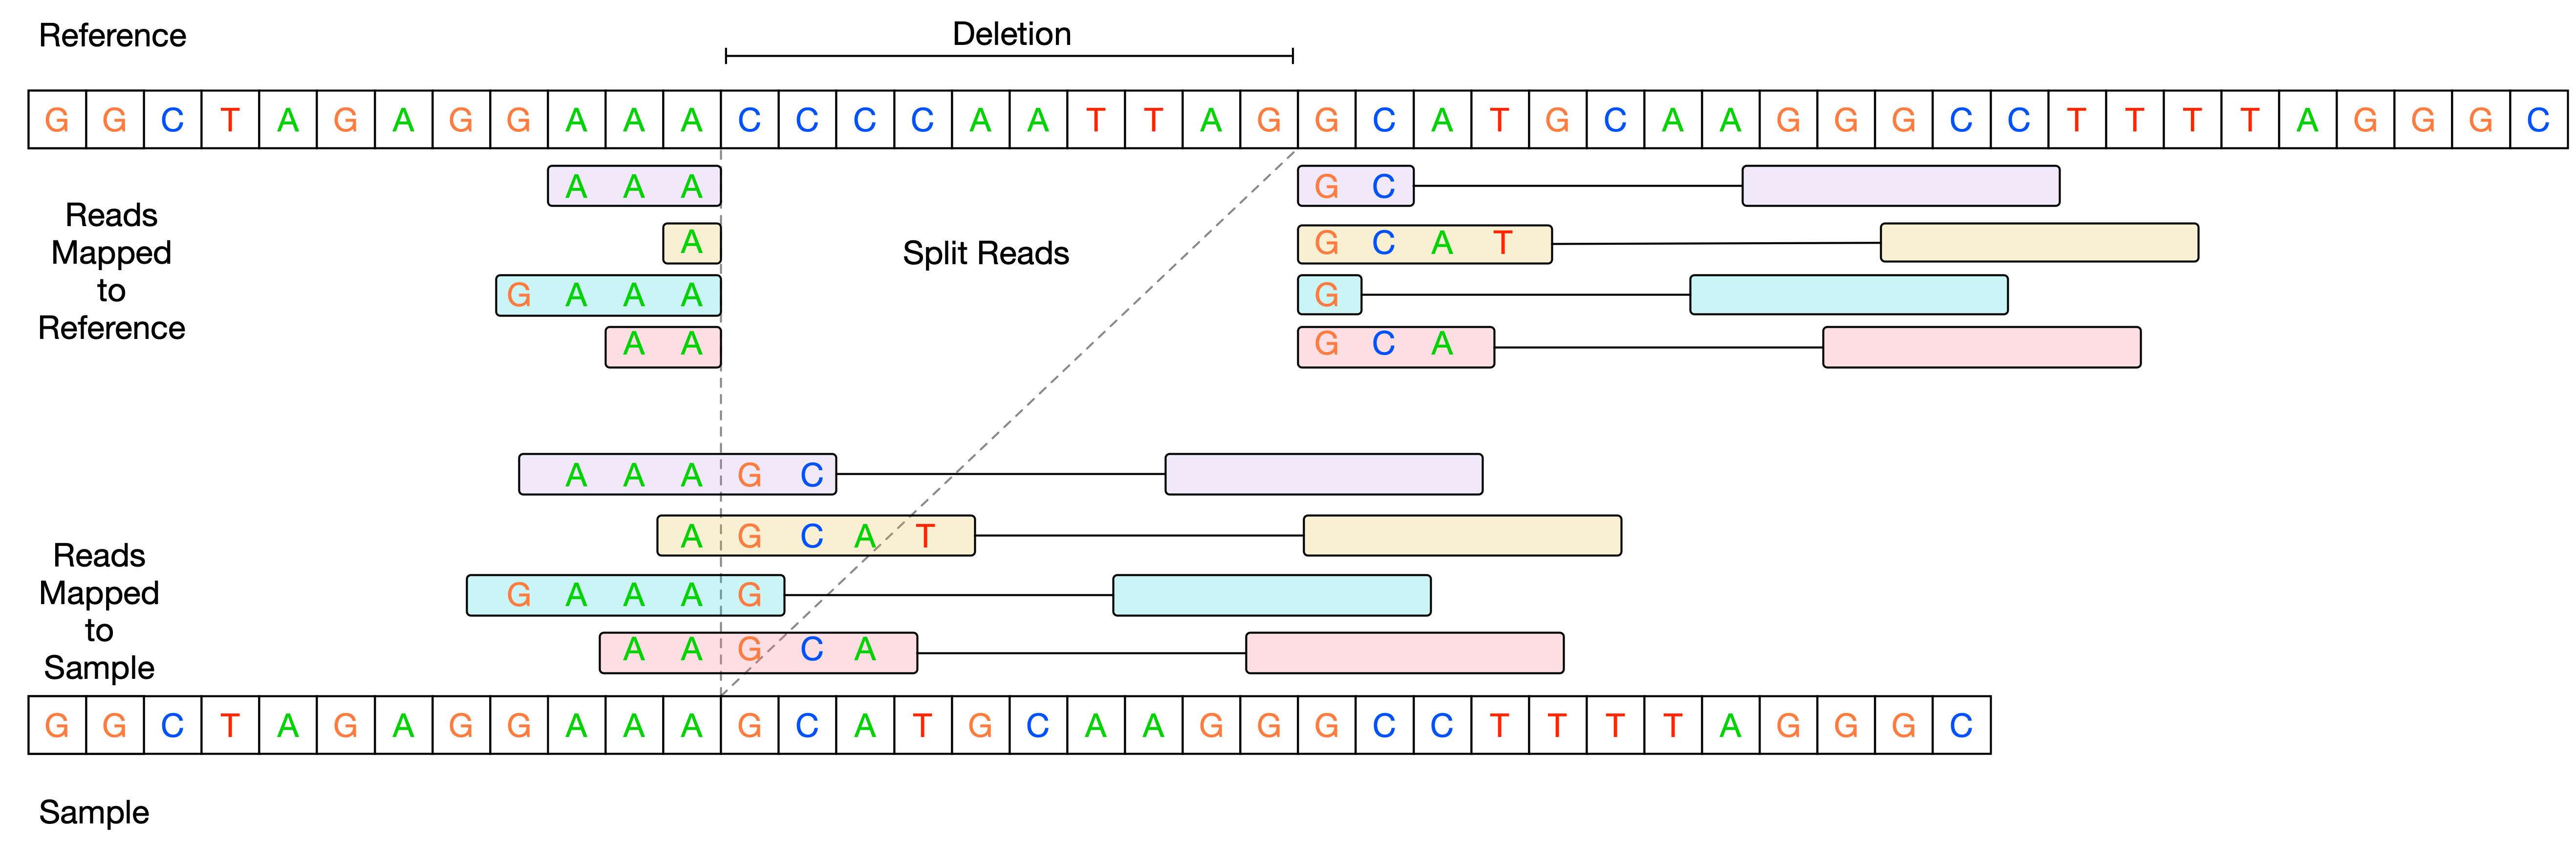
\includegraphics[scale=0.33]{split_reads}
    \centering
    \caption {Split-reads at the site of a deletion breakpoint.}
    \label{fig:split_reads}
\end{figure}

Although the techniques used for single read mapping, described above, can be used for split-read alignment there are several issues to consider that make the creation of a separate $mapSplitReadToReference()$ operation desirable. 

Since a split-read consists essentially of two or more separate pieces of varying lengths that may map to distant locations in the genome and have different orientations, determining where to "split" the read affects the quality of the subsequent mapping, as improper splits will generate many mismatches. $mapToReference()$ is intended to be optimized for speed on well-behaved reads which constitute most of the data that is seen for a given sample, but as a result make a number of assumptions, such as a single k-mer size and co-linearity of matches, that are invalid or sub-optimal for split-read alignment. Furthermore, the data representation for an aligned read in $mapToReference()$ of a single sequence $b$ of bases, $q$ of base qualities, and $cigar$ string representing the alignment is not well suited to representing an alignment consisting of multiple, possibly distant, pieces of possibly different orientations, as this is not readily representable in CIGAR. 

In current software that relies on writing SAM files as a medium for alignments, split-reads are represented as multiple records with the same ID, where one record is arbitrarily chosen to be primary (or representative) and others are marked supplementary (via an 0x800 FLAG value). Each record represents a separate piece of the split read where the unmatched portion is masked out via soft-clipping in the CIGAR string or is hard-clipped (see Section \ref{sec:bg_file_formats} for details on the SAM format). The details of the split-read alignment are captured in each read's optional SA tag in the form of a semi-colon separated list of strings that describe the supplementary alignments. In Figure \ref{fig:igv_split_read}, for example, there is a split read pictured that was obtained from a sample on chromosome 20 of the NA12878 individual in the 1000 Genomes Project, aligned by BWA-MEM, where one portion of the read aligns on the positive(+) strand, while another portion of the read aligns on the negative(-) strand some distance away. The yellow area in the figure describes the first part of the read which is labeled primary. The read is 250 basepairs long and the CIGAR string is 68S81M101S, indicating 68 soft-clipped bases, followed by an 81 basepair match to the reference, and followed by another 101 soft-clipped bases. The 101 basepair segment has low base quality, so it likely consists primarily of sequencing errors, but the 81 basepair segment has base qualities around 30, which is relatively high. The SA tag reads - SA:Z:20,42589216,-,179S71M,60,0;, indicating that there is a secondary alignment mapped to chromosome 20, starting at position 42589216, on the negative strand, with CIGAR string 179S71M (179 soft-clipped bases followed by a 71 basepair match to the reference). This is indeed the case and the corresponding read is pictured in Figure \ref{fig:igv_split_read} shaded purple. Investigating the SAM record for this mapping reveals that the actual record has CIGAR string 179H71M, i.e. the bases at the beginning are actually hard-clipped, not soft-clipped (soft-clipped bases are excluded from the alignment but the sequence is still preserved in the file record, whereas hard-clipped bases are excluded from alignment and the sequence is not recorded in the file). Such a split-read might imply the presence of deletion proximal to an inversion in the sample with respect to the reference sequence, although the evidence from the read should be investigated in light of the evidence from all of the other reads that overlap this locus to make an accurate determination of the presence of a potential variant in that location.

\begin{figure}[H]
    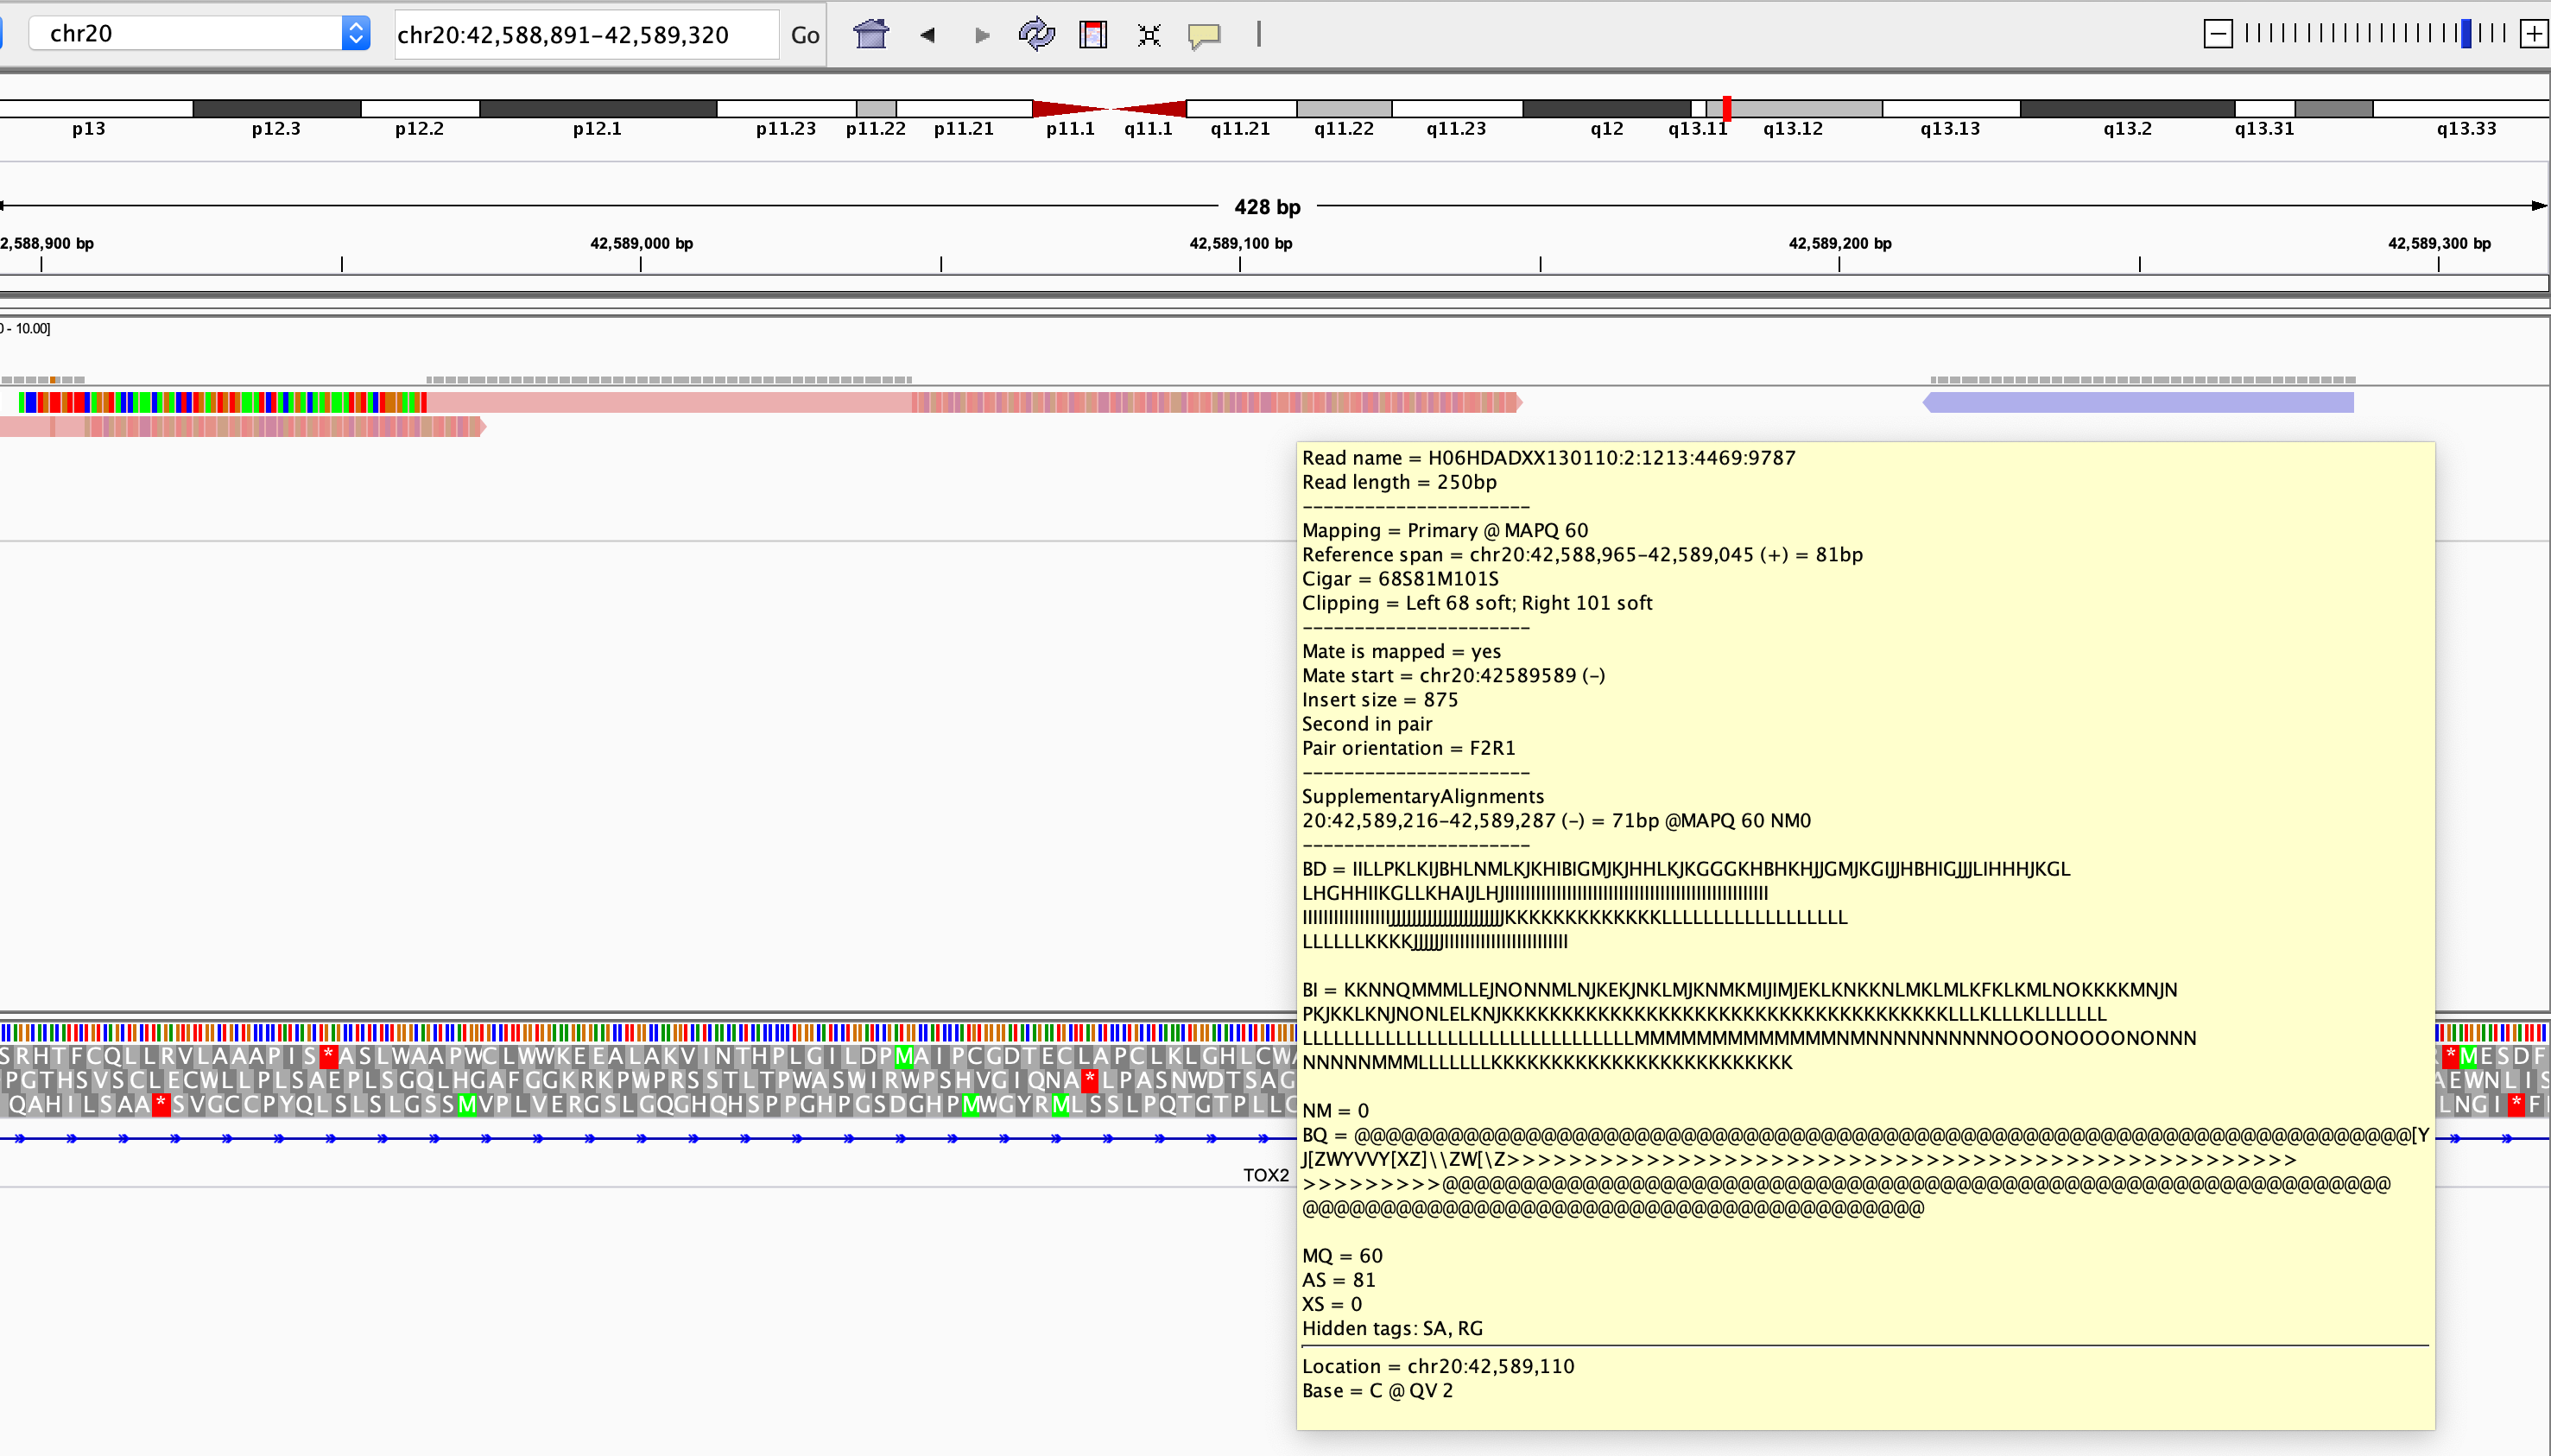
\includegraphics[scale=0.285]{igv_split_read}
    \centering
    \caption {IGV viewer rendering of a split-read on chromosome 20 from NA12878 sample.}
    \label{fig:igv_split_read}
\end{figure}

There are several issues with this scheme in addition to the apparent disagreement between duplicated information in the two records. The duplication is wasteful of space, and prone to errors as demonstrated above. There is no apparent ordering of the segments of the read that map to different locations because the next or previous segment are not specified for a given record, instead all secondary records point back to the primary. There is no well defined schema for the optional SA tag other than specifying a record separator. Thus, formats and contents of the encoding may vary between tools and even from record to record, without the ability to validate correctness of the encoding. Additionally, because the records in the SAM file are typically either in random order or coordinate-sorted order, the records for a split-read are not easily locatable and in the worst-case the entire file may need to be scanned in order to get the full split-read alignment for a single read. 

As Rheos does not rely on traditional genomics file formats for encoding, we chose a split-read representation that alleviates the issues above and encodes the entirety of a split-read alignment in a single record. Define:

\begin{equation}
    \label{eq:split_read}
    r_{split} = (s\_id, ref\_id, r\_id, b, q, f_p, aln)
\end{equation}

Here $s\_id, ref\_id, r\_id, b, q, f_p$ are as in Equation \ref{eq:raw_read_message} defining a raw read. $aln = (a_1,a_2,...,a_n)$ - an ordered list of alignment segments, where each \\$a_i = (i, rname, pos, offset, len, mapq, cigar, strand, flags)$, and:

\begin{description}
    \item[i] - ordinal number of $a_i$ in $aln$.
    \item[rname] - name of reference contig to which $a_i$ maps.
    \item[pos] - position on $rname$ where $a_i$ maps.
    \item[offset] - offset on $r_split$ where $a_i$ begins.
    \item[len] - length of $a_i$.
    \item[mapq] - mapping quality.
    \item[cigar] - CIGAR of the alignment.
    \item[strand] - alignment strand, 0 for positive, 1 for negative. Strand disagreement between $r_{split}$ and $a_i$ indicates sequence inversion.
    \item[flags] - various flags as in SAM format.   
\end{description}

\bgroup
\def\arraystretch{1.5}
\begin{table}[!ht]
    \caption{Definition of $mapSplitReadToReference()$}
    \label{tab:op_map_split_read_to_reference}
    {\begin{tabular}{l|p{12cm}}
    \toprule
    Inputs & \hangindent=1em$M_{unaln} = \{m_i: m_i = (header, r)\}$ where $r = (s\_id, r\_id, b, q, f_p, unmapped=true)$.\\
    \cline{2-2}
    Operation & $mapSplitReadToReference(r, ref\_id)$\\
    \cline{2-2}
    \multirow{2}{*}{Outputs} & \hangindent=1em$M_{split} = \{m_i: m_i = (header, r)\}$ where $r$ is as defined in Equation \ref{eq:split_read}.\\
    & \hangindent=1em $M_{unaln} = \{m_i: m_i = (header, r)\}$ where $r = (s\_id, r\_id, b, q, f_p, unmapped=true,split\_align=false)$\\
    \bottomrule
    \end{tabular}}
\end{table}
\egroup

The split-read alignment operates on reads that emerge unmapped from the regular alignment stage via $mapToReference()$. Alignment proceeds using the same general FM Index based framework as $mapToReference()$ but here each read is broken down into a series of progressively smaller k-mers. Each k-mer is aligned individually, and the alignment that maximizes aggregate alignment score across all k-mer sizes and candidate alignments is chosen. 

The alignment operations that have been considered in this section present a set of distinct challenges on the basis of 
the gamut of query sequence and reference database size combinations. Each scenario presented admits optimization with respect to its specific parameters. Existing aligners typically attempt to solve all or most of these problems with a single approach, and thus suffer from inability to fully optimize each specific use case. Our treatment, that separates the different alignment scenarios into distinct operations, with well delineated optimization criteria, and even into potentially separate services that may run on separate physical machines, allows us to fully optimize each operation without negatively impacting others.

\subsection{Simple Germline SNP Calling}\label{sec:main_body_germline_snp_calling}

SNPs are the most abundant and widely studied type of genetic variant\autocite{10002010map}. Section \ref{sec:bg_germline_snp_calling} provides an overview of existing methods for germline SNP calling. For a human diploid sample when calling variants on one of the autosomes (chromosomes 1-22), germline SNP calling comes down to selecting between three alternative models for each genomic locus based on the set of reads that are observed - homozygous reference, heterozygous, or homozygous variant (see Figure \ref{fig:snps}).   

\begin{figure}[H]
    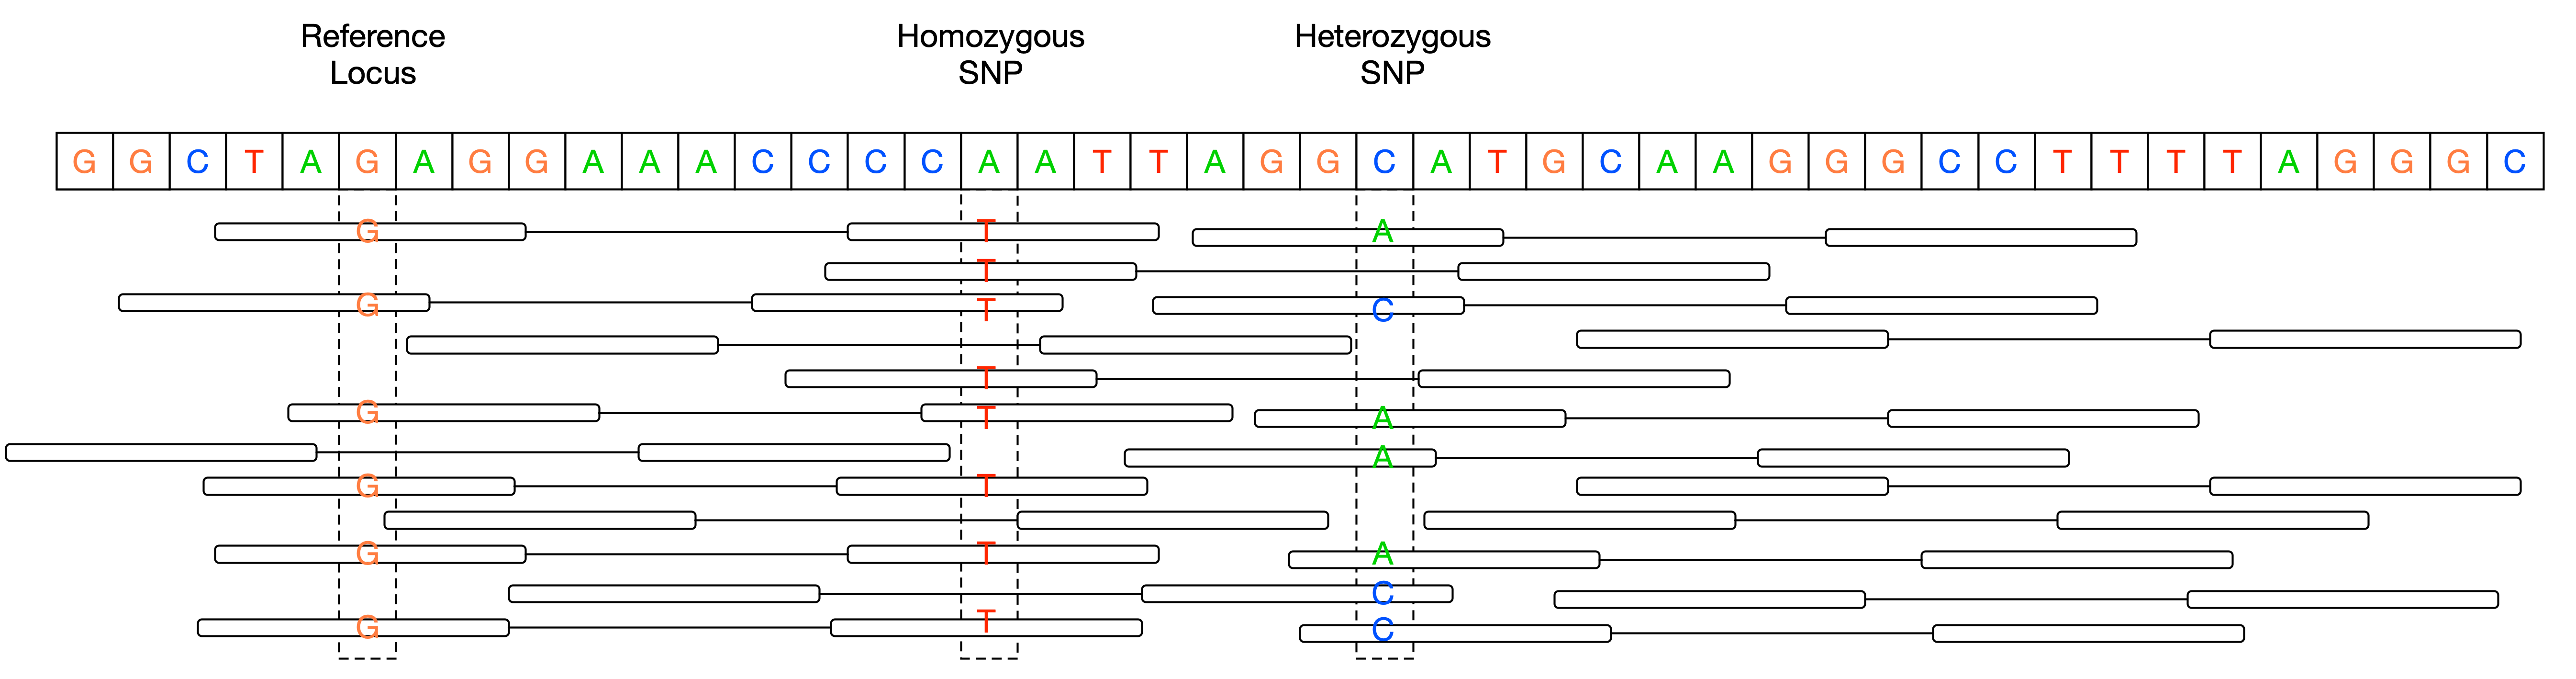
\includegraphics[scale=0.325]{snps}
    \centering
    \caption {Examples of genomic loci that match the reference sequence, have a heterozygous SNP, and a homozygous SNP.}
    \label{fig:snps}
\end{figure}

Although the most accurate currently available variant callers model the region around a SNP via local assembly of haplotypes\autocites{depristo2011framework}{rimmer2014integrating}{garrison2012haplotype}, a simpler approach assumes that every locus is independent and can still achieve high accuracy. For instance, samtools\autocite{li2011statistical}, which makes the independence assumption, has recently been compared to several local assembly based methods in \autocite{li2018synthetic} and was shown to have a slightly higher false-negative rate than platypus, freebayes, and Haplotype Caller, but also a slightly lower false-positive (FPPM = false positives per million bases) rate (see Figure \ref{fig:fb_hc_st_pt}). Additionally, in \autocite{rimmer2014integrating} Table 1, samtools has the highest sensitivity, but also the highest false discovery rate (FDR) on SNPs. Thus, the simpler independent locus model should be sufficient for calling germline SNPs and is of interest in the context of the data streaming approach of Rheos.

The random order in which reads appear in a Rheos data stream means that a new approach is required to successfully implement germline SNP calling on this data. Specifically, all of the existing tools for variant calling assume that all of the reads for a given sample have been observed, mapped to the reference, sorted by increasing reference coordinate, and stored in a SAM or BAM file. Variant calling (see Section \ref{sec:bg_germline_snp_calling}) proceeds by traversing the data in a coordinate-ordered fashion, loading all of the reads that overlap a given locus into memory, into a structure called a read pileup (see Figure \ref{fig:main_body_locus}), and evaluating a set of alternative models for each locus, typically in a Bayesian framework, selecting either the maximum-likelihood estimate (MLE) or the maximum a posteriori (MAP) estimate as the called genotype.

\begin{figure}[H]
    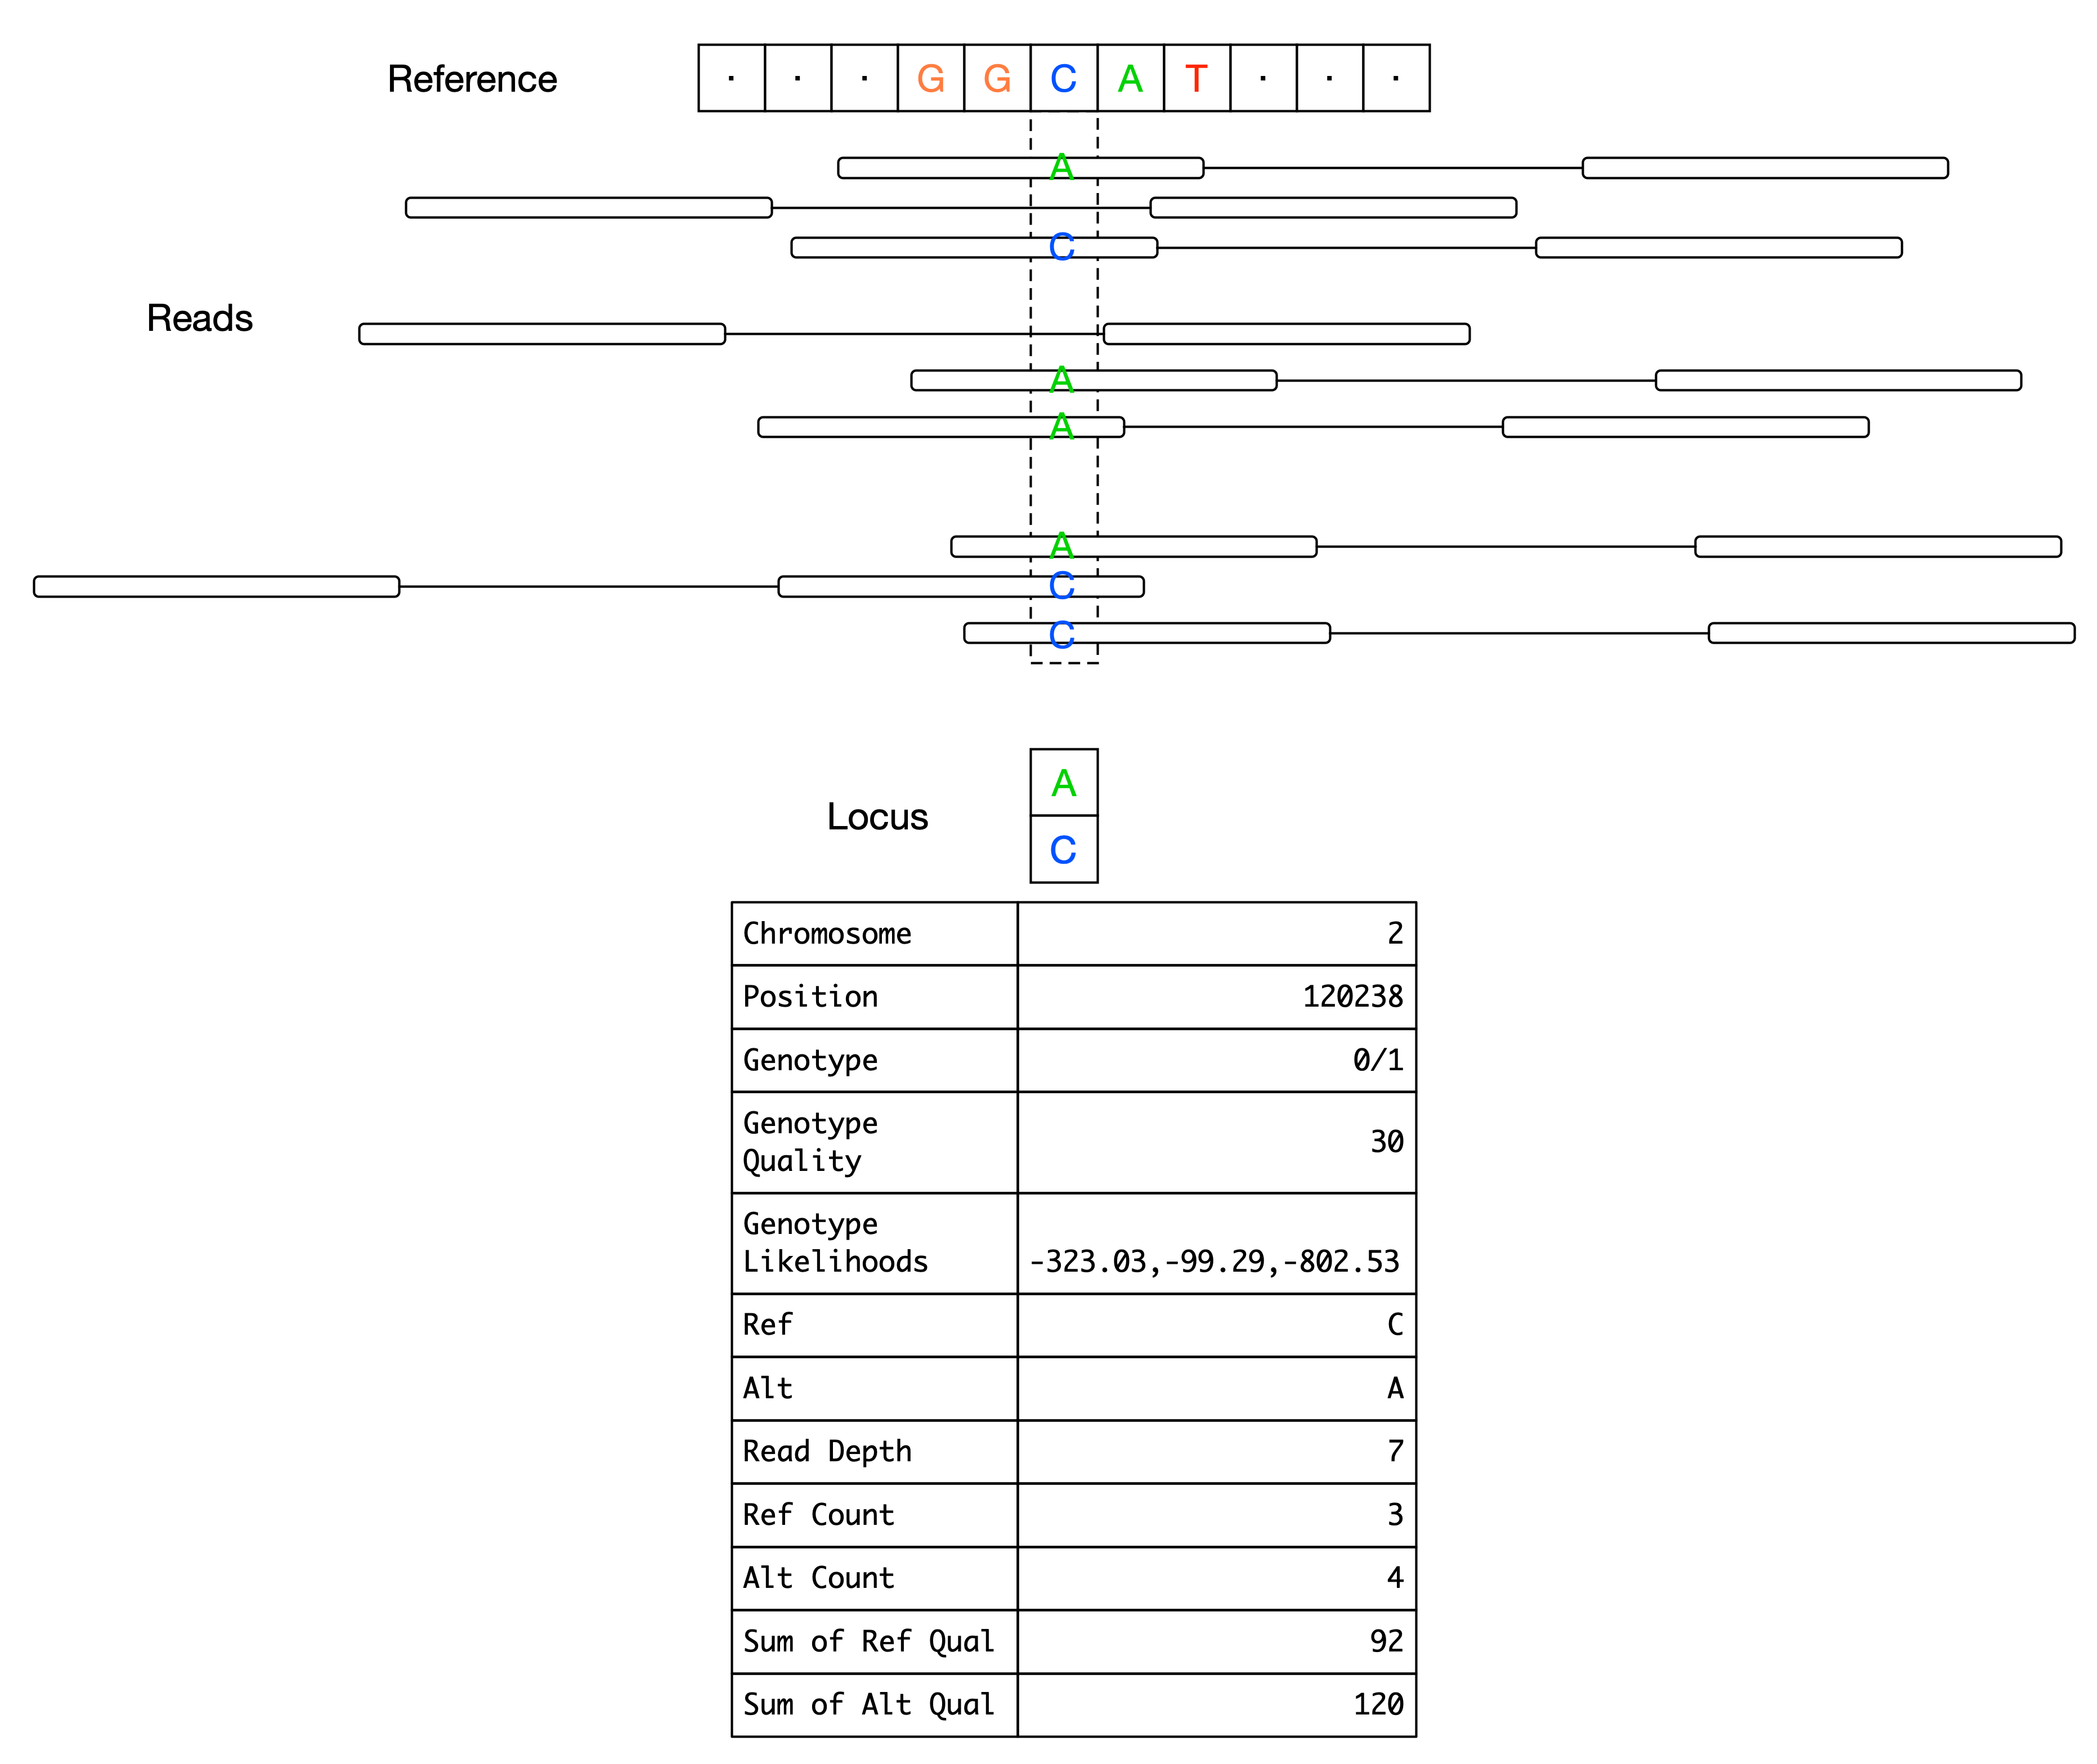
\includegraphics[scale=0.325]{locus}
    \centering
    \caption {A read pileup over a locus with a heterozygous SNP.}
    \label{fig:main_body_locus}
\end{figure}

The Bayesian framework that is typically adopted follows this form (see also Section \ref{sec:bg_gatk}):

\begin{equation}
    \label{eq:main_body_gatk_genotyping}
P(G|D) = {P(G)P(D|G)\over\sum_i P(G_i)P(D|G_i)}
\end{equation}

Here some prior distribution $P(G)$ of genotypes at a locus is assumed. This can be an uninformative prior (for instance one that assigns equal probability to all possible genotypes), or it can be a prior based on a population genetics model, or empirically obtained distribution of genotypes in a given population. The genotype likelihood $P(D|G)$ under assumptions of independent observations (reads) and independent errors, factors into a product of individual observation likelihoods i.e. $P(D|G) = \prod_j{P(D_j|G)}$. Each observation $P(D_j|G)$ is further subject to a sequencing error probability $\epsilon_j$, derived from the recorded base quality for the read over the locus being considered. Thus, $P(D_j|G) = 1 - \epsilon_j$ when $D_j = G$ and $P(D_j|G) = \epsilon_j$, otherwise. Genotype likelihoods are then computed as in Equations \ref{eq:samtools_diploid_genotype_likelihoods} for samtools, and similarly Equations \ref{eq:freebayes_main_model}, \ref{eq:freebayes_afs}, \ref{eq:freebayes_obs_given_base} for freebayes, Equation \ref{eq:gatk_genotype_likelihood} for GATK, and Equation \ref{eq:platypus_likelihood_model} for platypus. A site is called variant if the probability of having at least one non-reference allele at the locus exceeds the probability of having 0 non-reference alleles. A genotype is assigned if the ratio of the genotype with the highest likelihood to the genotype with the second highest likelihood exceeds some pre-determined constant, i.e., assuming genotype $g \in [0,1,2]$ denotes the number of reference alleles at the locus, and, for example, given $\mathcal{L}(g_2) > \mathcal{L}(g_1) > \mathcal{L}(g_0)$, assign the genotype $g=2$ if $\frac{\mathcal{L}(g_2)}{\mathcal{L}(g_1)} > c$, where $c > 1$ is some user-set threshold. The calling proceeds locus-by-locus in coordinate-ordered fashion, and the results are written to a file in VCF format (see \ref{sec:bg_file_formats}) where each row represents a variant.

The process above is efficient in that each locus is looked at only once in order to be able to make a call, but it is inefficient in that all of the data needs to have been observed, mapped, and sorted in order to even begin calling. The streaming approach that we adopt in Rheos allows us to begin calling immediately as we start seeing data, in return for needing to re-evaluate a locus multiple times as new data arrives. Because each read is immediately integrated into the model once it is observed, the state of our model of the genome is at all times consistent with all of the read evidence that has been observed to date. Each locus then simply provides an estimate of the underlying genotype based on the data that is available at that time. Initially, these estimates may be inaccurate, but accuracy improves as more and more data arrives and the estimates are refined in an iterative fashion.   

We are thus interested in an iterative update rule that, given a current set of genotype likelihood estimates at a locus, that incorporate evidence from $n$ reads that have already been observed, when the read $n+1$ arrives, is able to produce an updated set of genotype likelihoods that is consistent with evidence from all $n+1$ reads, as well as any other auxiliary structures necessary for producing a variant call record. To do this we adopt a sequential Bayesian framework, where the posterior distribution of genotype likelihoods at step $n$ becomes the prior (albeit unnormalized) for step $n+1$. 

Let:

\begin{table}[!h]
    \label{tab:snp_calling_notation}
    {\begin{tabular}{lp{11cm}}
    \toprule
    Symbol & Description \\
    \midrule
    $R$ & The reference sequence. \\
    $S$ & The sample sequence. \\
    $D = \{d_i: i \in [1,n]\}$ & The set of $n$ observations seen to date. \\ 
    $d_i$ & $i$'th read observation. \\
    $g_{i}$ & Genotype of sample $S$ at locus $i$. $g \in [0,1,2]$ counts the number of reference alleles at locus $i$\\
    $P_n(G_i)$ & Probability of genotype $G = g$ at locus $i$, after seeing $n$ observations $d$ that overlap locus $i$.\\
    $\mathcal{L}(d_n|G_i)$ & Genotype likelihood function at locus $i$ for the $n$'th observation.\\
    \bottomrule
    \end{tabular}}
\end{table}

We take $P_0(G_i)$ to be the prior probability of $G$ at $i$. After observing the first data point $d_1$ which has base quality (probability of error) $\epsilon_1$, we calculate:

\begin{align*}
&\mathcal{L}(d_1|G=0) = 1 - \epsilon_1\\
&\mathcal{L}(d_1|G=1) = \frac{1}{2}\\
&\mathcal{L}(d_1|G=2) = \epsilon_1
\end{align*}

if $d_1$ is different from reference, and:

\begin{align*}
&\mathcal{L}(d_1|G=0) = \epsilon_1\\
&\mathcal{L}(d_1|G=1) = \frac{1}{2}\\
&\mathcal{L}(d_1|G=2) = 1 - \epsilon_1
\end{align*}

if $d_1$ matches the reference. Consequently, by Bayes' Rule:

\begin{align*}
&\mathcal{L}(G=0|d_1) \propto \mathcal{L}(d_1|G=0) * P_0(G=0)\\
&\mathcal{L}(G=1|d_1) \propto \mathcal{L}(d_1|G=1) * P_0(G=1)\\
&\mathcal{L}(G=2|d_1) \propto \mathcal{L}(d_1|G=2) *  P_0(G=2)
\end{align*}

Now, assuming that we have observed $n$ data points and calculated $\mathcal{L}(G|D_n)$ (likelihood of genotype given $n$ data points $D_n$). We obtain a new data point $d_{n+1}$ and calculate:

\begin{align*}
&\mathcal{L}(d_{n+1}|G=0) = 1 - \epsilon_1\\
&\mathcal{L}(d_{n+1}|G=1) = \frac{1}{2}\\
&\mathcal{L}(d_{n+1}|G=2) = \epsilon_1
\end{align*}

if $d_{n+1}$ is different from reference, and:

\begin{align*}
&\mathcal{L}(d_{n+1}|G=0) = \epsilon_1\\
&\mathcal{L}(d_{n+1}|G=1) = \frac{1}{2}\\
&\mathcal{L}(d_{n+1}|G=2) = 1 - \epsilon_1
\end{align*}

if $d_{n+1}$ matches the reference. Using this likelihood and the posterior from step $n+$ as the prior for step $n+1$, again by Bayes' Rule, we obtain:

\begin{align*} 
&\mathcal{L}(G=0|D_{n+1}) \propto \mathcal{L}(d_{n+1}|G=0) * \mathcal{L}(G=0|D_{n})\\
&\mathcal{L}(G=1|D_{n+1}) \propto \mathcal{L}(d_{n+1}|G=1) * \mathcal{L}(G=1|D_{n})\\
&\mathcal{L}(G=2|D_{n+1}) \propto \mathcal{L}(d_{n+1}|G=2) * \mathcal{L}(G=2|D_{n}) \numberthis \label{eq:rheos_genotype_likelihood}
\end{align*}

Equation \ref{eq:rheos_genotype_likelihood} provides the general update rule for incorporating new evidence about a given locus $i$ having already made and recorded $n$ observations, upon making observation $n+1$. This iterative approach is mathematically equivalent to the batch update approaches such as \autocite{li2011statistical}, that collect all of the data about a locus before evaluating genotype likelihoods. The posteriors obtained by equation \ref{eq:rheos_genotype_likelihood} can be used directly to evaluate relative likelihoods of the possible genotypes, and to assign genotypes via a likelihood ratio, for example, but in order to obtain a proper posterior probability mass function over the genotypes they need to be normalized, to obtain:

\begin{equation} \label{eq:rheos_genotype_posterior}
    P(G=g|D) = \frac {\mathcal{L}(G=g|D)} {\sum_{g'\in G} \mathcal{L}(G=g'|D)}
\end{equation}

This equation can be used to obtain a probability estimate of any given genotype, having observed any given amount of data about a specific locus.

Armed with the update rule for integrating read evidence we are ready to define a data stream operation of Local State Aggregator type that is responsible for processing a stream of aligned read pairs, updating its local state with the genetic variation evidence contained in the reads, and emitting a stream of updated genomic loci (see Fig. \ref{fig:main_body_locus}) that can be used by downstream services for variant calling.

\bgroup
\def\arraystretch{1.5}
\begin{table}[!ht]
    \caption{Definition of $updateLociFromRead()$}
    \label{tab:op_update_loci_from_read}
    {\begin{tabular}{l|p{12cm}}
    \toprule
    Inputs & \hangindent=1em$M_{aln} = \{m_i: m_i = (header, payload)\}$ where $m.payload = (r_1,r_2)$ and each read is of type $r_{aln}$. \\
    \cline{2-2}
    Operation & $updateLociFromRead(r, ref, current_loci)$\\
    \cline{2-2}
    Outputs & \hangindent=1em$M_{loci} = \{m_i: m_i = (header, L)\} \text{ where } L = \{l : l=(s\_id, ref\_id, contig, pos, alt, gl_0, gl_1, gl_2, dp, ro, qr, ao, qa)\}$\\
    \bottomrule
    \end{tabular}}
\end{table}
\egroup

A Locus $l$ for SNP calling represents a single genomic location for a single sample and a particular reference genome. For each Locus we keep track of the following fields:

\begin{description}
    \item[s\_id] - Sample ID.
    \item[ref\_id] - Reference Genome ID.
    \item[contig] - Name of the reference contig.
    \item[pos] - Reference-relative position of the Locus on the contig.
    \item[alt] - The alternative allele at this locus (if any alternative alleles have been observed).
    \item[gl\_0] - Likelihood of homozygous alternative genotype at this locus, based on the data seen so far.
    \item[gl\_1] - Likelihood of heterozygous genotype at this locus, based on the data seen so far.
    \item[gl\_2] - Likelihood of homozygous reference genotype at this locus, based on the data seen so far.
    \item[dp] - Read depth - number of reads observed at this locus so far.
    \item[ro] - Number of reference observations at this locus.
    \item[qr] - Sum of base qualities of reference observations at this locus.
    \item[ao] - Number of alternative observations at this locus.
    \item[qa] - Sum of base qualities of alternative observations at this locus.       
\end{description}

\paragraph{The Locus Processing Service} which is responsible for implementing $updateLociFromRead()$ maintains a local data store of Locus objects, ideally in memory. When a new mapped read arrives via the input stream, the service walks along the read and for each position on the read compares it to the respective position on the reference sequence. It retrieves the Locus corresponding to this position and, depending on whether the read matches, or is different from the reference sequence, updates the Locus genotype likelihoods (and other fields) according to the update rule of Equation \ref{eq:rheos_genotype_likelihood}. Those Locus objects that have been updated, and have alternative allele observations (i.e. potential variants) are added to a list of objects that should be emitted by the service as output of $updateLociFromRead()$. Since a read alignment consists of not only matches and mismatches with respect to the reference sequence, but also encodes insertions and deletions as an array of CIGAR elements (see \ref{sec:bg_alignment}), and the alignment may occur on the forward or the reverse strand of DNA (requiring reverse complementing) special care needs to be taken during read processing to account for all of the possible cases of simultaneous read and reference traversal. Read processing proceeds as in the following algorithms:

\begin{algorithm2e}[h]
    \DontPrintSemicolon
    \footnotesize
    \textbf{Function} {\sc processReadPair}$(read\_pair, ref)$
    \Begin {
        \For{$read$ {\bf in } $read\_pair$}{
            $strand \gets read.strand$\;
            $cigar\_els \gets read.cigar\_els$\;
            $ref\_offset \gets 0$\;
            $read\_idx \gets read.query\_start$\; \tcc*{Alignment does not necessarily start at index 0.}\;

            \For{$el$ {\bf in} $cigar\_els$}{
                \If {$el.type = MATCH$ {\bf or } $ el.type = DEL$}{
                    \If {$el.type = MATCH$}{
                        $updated\_loci$ \gets {\sc handleMatch$(read, read\_idx, el.length, ref\_offest, ref)$}\;
                    }
                    $ref\_offset \gets ref\_offest + el.length * strand$\; \tcc*{both matches and deletions consume reference sequence. Reads that align on the negative strand consume reference backwards.}\;
                }

                \If {$el.type != DEL$ {\bf and } $el.type != SOFT\_CLIP$}{
                    $read\_idx = read\_idx + el.length$ \tcc*{All elements but deletions and soft-clips consume read sequence.}\;
                }
            }
        }
    }
    \caption{Process read and reference in tandem to find matching CIGAR elements.}\label{ag:process_read_pair}
\end{algorithm2e}

\begin{algorithm2e}[h]
    \DontPrintSemicolon
    \footnotesize
    \textbf{Function} {\sc handleMatch$(read, read\_idx, match\_length, ref\_offest, ref)$}
    \Begin {
        $seq \gets read.seq[read\_idx:read\_idx+match\_len]$\;
        $qual \gets read.qual[read\_idx:read\_idx+match\_len]$\;
        \If {$read.strand = 1$}{
            $ref\_start \gets read.position + ref\_offest - 1$\;
        }
        \Else{ \tcc*{When read is on negative strand sequence is reverse complemented and matching starts from end of reference.}
            $seq \gets ${\sc reverseComplement$(seq)$}\;
            $ref\_start \gets read.end + ref\_offest - match\_length - 1$\;
        }
        $read\_ref \gets ref[ref\_start: ref\_start+match\_length]$\;
        \For{$pos\_idx$ {\bf in} $seq$}{
            $cur\_ref \gets ref\_start + pos\_idx$\;
            $cur\_locus \gets ${\sc all\_loci.getLocus$(cur\_ref)$}\;
            $p\_error \gets ${\sc baseQualityToProbabilityOfError$(qual[pos\_idx])$}\;
            $cur\_locus.dp \gets cur\_locus.dp + 1$\;
            $cur\_locus.gl\_het \gets cur\_locus.get\_het * 0.5$\;

            \If{$seq[pos\_idx] != ref[pos\_idx]$}{
                $cur\_locus.alt \gets seq[pos\_idx]$\;
                $cur\_locus.gl\_ref \gets cur\_locus.gl\_ref * p\_error$\;
                $cur\_locus.gl\_hom \gets cur\_locus.gl\_ref * (1 - p\_error$)\;
                $cur\_locus.ao \gets cur\_locus.ao + 1$\;
                $cur\_locus.qa \gets cur\_locus.qa * qual[pos\_idx]$\;
            }
            \Else{
                $cur\_locus.gl\_ref \gets cur\_locus.gl\_ref * (1 - p\_error$\;
                $cur\_locus.gl\_hom \gets cur\_locus.gl\_ref * p\_error$\;
                $cur\_locus.ao \gets cur\_locus.ro + 1$\;
                $cur\_locus.qa \gets cur\_locus.qr * qual[pos\_idx]$\;
            }            
        }
    }
    \caption{Process a portion of the read that maps to reference as a match, updating all loci that it overlaps.}\label{ag:handle_match}
\end{algorithm2e}

Algorithm \ref{ag:process_read_pair} is responsible for locating the genomic coordinates of those parts of the alignment that are flagged as matches (a match may still have differences from the reference). This is accomplished by traversing the CIGAR elements of the alignment and updating the coordinate offset of the read, the reference, or both, depending on the type of CIGAR element that is encountered. When a CIGAR element corresponding to a match is encountered it is processed by Algorithm \ref{ag:handle_match}, which is responsible for updating the set of loci that the matching region overlaps with the evidence for (or against) variation that exists in the read. In Algorithm \ref{ag:handle_match}, the DNA strand to which the read maps determines whether the read sequence needs to be reverse complemented and whether the match offsetting proceeds from the beginning or the end of the reference sequence. After offsets are computed the actual matching always proceeds moving forward (in the direction of increasing coordinates) along the reference sequence. At each location the reference and read sequences are compared and the underlying Locus model is updated based on the update rule of Equations \ref{eq:rheos_genotype_likelihood}. Those loci that have a non-zero count of alternative allele observations are added to a list of loci that potentially harbour variants and will be emitted from the Locus Processing Service as a stream $M_{loci}$ for further downstream processing by the variant caller.

\paragraph{The Variant Calling Service} - is responsible for actually making SNP variant calls based on a set of user-defined calling criteria, such as a region of interest, variant quality, genotype likelihood, number of supporting observations, etc. The service translates between a set of Locus models maintained by Rheos and an external data format (namely VCF). This service does not operate on a stream of data, but instead acts as a query service that can be invoked by the user ad hoc with specified parameters to answer queries of interest.

\bgroup
\def\arraystretch{1.5}
\begin{table}[!ht]
    \caption{Definition of $callVariants()$}
    \label{tab:op_call_variants}
    {\begin{tabular}{l|p{12cm}}
    \toprule
    Operation & $callVariants(region, calling\_threshold)$\\
    \cline{2-2}
    Outputs & \hangindent=1em$outputVCF$\\
    \bottomrule
    \end{tabular}}
\end{table}
\egroup

For each locus inside the queried region the Variant Calling Service evaluates the set of genotype likelihoods at that locus and calculates normalized genotype posterior probabilities using Equation \ref{eq:rheos_genotype_posterior}. The variant quality is defined to be the Phred-scale transformed probability that a site is homozygous reference, i.e. sites that, based on the read evidence, have a very low probability of being reference, under the Phred-scale transformation end up with a high variant quality (see Equation \ref{eq:samtools_variant_quality}). Variants that exceed $calling\_threshold$ will be emitted as records to the output VCF file. It is possible to envision more sophisticated versions of the Variant Calling Service that provide extended querying and filtering capabilities.

\subsection{Germline Structural Variant Calling}\label{sec:main_body_sv_calling}

As Rheos aims to provide comprehensive sample characterization it is not enough to only be able to call single nucleotide polymorphisms, the ability to call other variants, such as indels and structural variants is also required. Here we examine an approach for calling a specific class of structural variants, namely deletions, using a stream of mapped read pairs made available by the Read Mapping Service's $mapPairToReference()$ operation. 

In general, structural variant callers typically make use of three types of evidence for the presence of structural variation - read depth, discordantly mapped reads, and split-reads (see Section \ref{sec:bg_germline_sv_calling}). Here we utilize discordantly mapped reads i.e. those read pairs that align farther away from each other than expected in order to assess the presence of sequence deletions in the sample with respect to the reference.

\begin{figure}[H]
    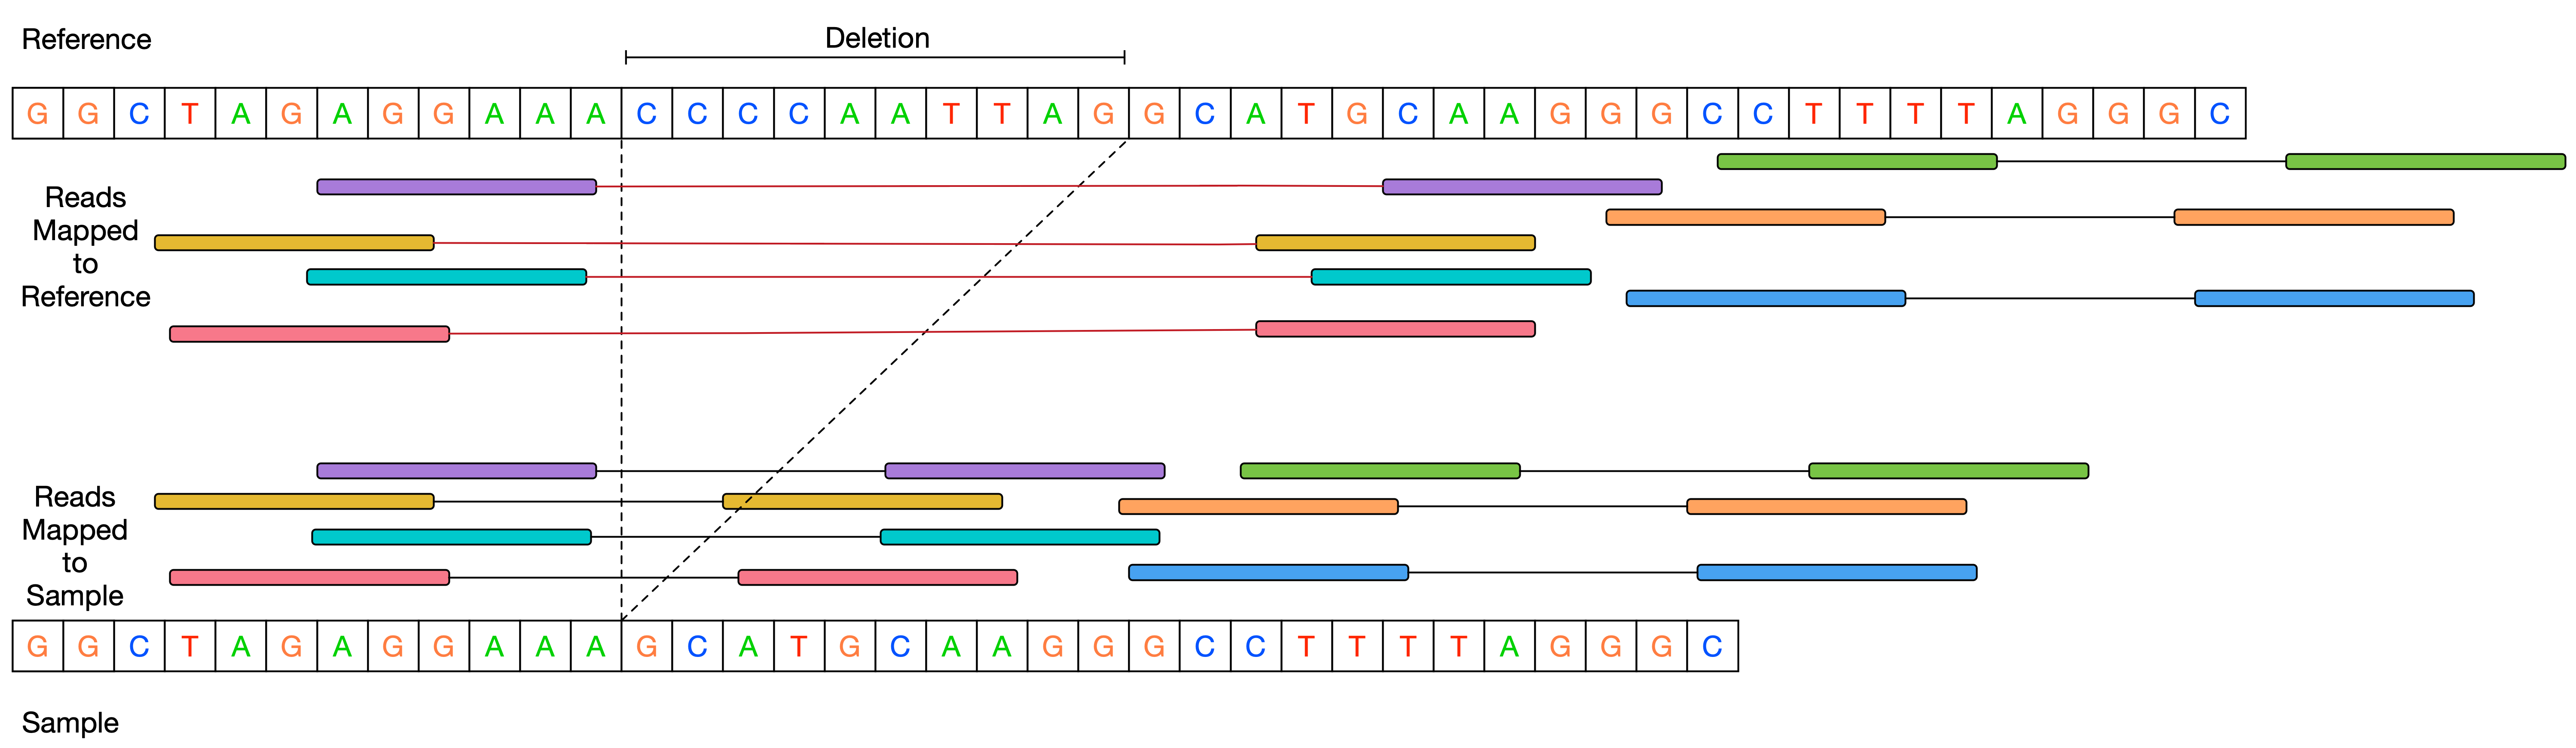
\includegraphics[scale=0.295]{sv_deletion}
    \centering
    \caption {Effect on read-pair mapping distance for reads overlapping a deletion.}
    \label{fig:sv_deletion}
\end{figure}

In Figure \ref{fig:sv_deletion} the sample being sequenced has a deletion with respect to the genome reference, namely the sequence "CCAAATTAG" is deleted. When sequencing with read pairs, the term "insert size" refers to the size of a DNA fragment that is being sequenced, less the size of the sequence adapters on both ends(see \ref{fig:insert_size}). Thus, assuming that both reads in a pair have been mapped, and have mapped in the proper orientations (5' towards 3' on both strands). If the Read Mapping Service emits the read pair as $(r_1, r_2)$ where $r_i$ are as previously defined and $r_1.pos$, $r_1.end$, $r_2.pos$, $r_2.end$, and assuming without loss of generality that $r_1$ is the read that maps on the positive strand, then the insert size $l_{r_1,r_2} = r_2.end - r_1.pos$.    

\begin{figure}[H]
    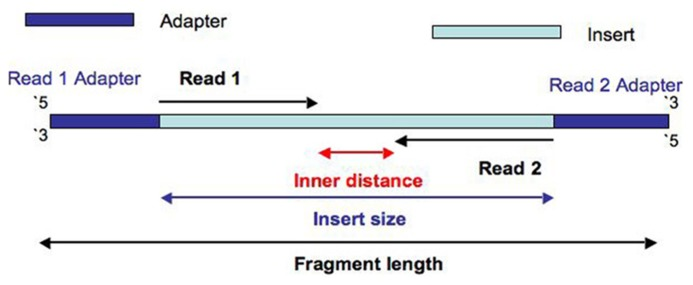
\includegraphics[scale=4]{insert_size}
    \centering
    \caption {Read-pair insert size is the size of the DNA molecule being sequenced minus the length of adapters on both sides\autocite{turner2014assessment}.}
    \label{fig:insert_size}
\end{figure}

As can be seen from Figure \ref{fig:sv_deletion}, for those reads that span the site of the deletion the inferred insert size is larger than the actual insert size (approximately by the size of the deletion), since the read are mapped farther apart on the reference than they are on the sample. Such read pairs are said to be discordantly mapped. Since the insert size distribution for a given sample is relatively predictable (see Figure \ref{fig:insert_size_distribution}), it is possible to detect the presence of deletions in a sample by identifying clusters of read pairs that have an inferred insert size larger than some predefined threshold. Such an approach is already used by several structural variant callers\autocites{rausch2012delly}{layer2014lumpy} and we adopt it in Rheos with several key innovations.

Detection proceeds in two stages performed by two different services. The Insert Size Filtering Service is responsible for listening to the general stream of read pairs and filtering out all of the pairs that don't meet the requisite criteria. The Insert Size Clustering Service is responsible for consuming a stream of discordantly mapped read pairs, clustering the reads that are located close to each other, and outputting those clusters that have sufficient evidence for being considered sites of deletions.

For the Insert Size Filtering Service we define the following operation:

\bgroup
\def\arraystretch{1.5}
\begin{table}[!ht]
    \caption{Definition of $filterDiscordantPairs()$}
    \label{tab:op_filter_discordant_pairs}
    {\begin{tabular}{l|p{12cm}}
    \toprule
    \multirow{2}{*}{Inputs} & \hangindent=1em$M_{aln} = \{m_i: m_i = (header, payload)\}$ where $m.payload = (r_1,r_2)$ and each read is of type $r_{aln}$\\
    \cline{2-2}
    \multirow{2}{*}{Operation} & $filterDiscordantPairs(r_1,r_2, min\_mapq, mad\_threshold, min\_sample\_size)$\\
     \cline{2-2}
    \multirow{2}{*}{Outputs} & \hangindent=1em$M_{disc} = \{m_i: m_i = (header, payload)\}$ where $m.payload = (r_1,r_2)$ and each read is of type $r_{aln}$\\
    \bottomrule
    \end{tabular}}
\end{table}
\egroup

Here, the $filterDiscordantPairs()$ operation subscribes to the stream of mapped read pairs that is produced by the Read Mapping Service. The goal is to produce a stream of read pairs that are suitable for clustering. The following conditions must be satisfied in order for a pair to be considered suitable:

\begin{description}
    \item [Both reads in a pair must be mapped] - the Read Mapping Service actually emits some read pairs where only one of the reads is mapped into the mapped reads stream.
    \item [Both reads in must be mapped to the same contig] - Read pairs where individual reads map to different contigs may be indicative of genomic translocations (another type of structural variant), but are not suitable for the detection of deletions, since different contigs are actually different physical molecules.
    \item [Both reads must have mapping quality $\ge$ min\_mapq] - A mapping quality of at least 30 (the default value) on the Phred scale, for instance, implies a probability of no more than $10^{-3}$ that a read is mapped to the wrong location on the reference.
    \item [Insert size must be > MAD * mad\_threshold] - the Median Absolute Deviation is taken as a measure of the central tendency of the distribution of insert sizes that is robust against extreme outliers, which can be quite common. Typical fragment size of the DNA that is being sequenced is in the hundreds of nucleotides long, whereas certain inferred insert sizes can reach millions of bases due to structural variants or spurious mappings. Thus, it is desirable to have a metric similar to variance that will not be sensitive to these extreme values. Given a set of insert sizes $L = \{l_i: l_i=r_2.end-r_1.pos \}$, define $MAD(L) = median(\mid l_i - median(L)\mid)$. The cutoff of mad\_threshold*MAD places a lower bound on the size of deletions that can be detected with this method. A value of 5 is arbitrarily chosen as the default for $mad\_threshold$.
\end{description}

Since obtaining an accurate estimate of median insert size and MAD requires observing a sample of read pairs, the Insert Size Filtering Service does not emit any reads at first, but accumulates observations in a local data store while collecting enough information to obtain reliable estimates of these metrics. $min\_sample\_size$ ($10^5$ by default) read pairs are collected before filtering begins. Once the metrics are obtained, collected reads are filtered first and released, before processing any of the remaining reads on the stream.

Read pairs that satisfy all of the conditions above are emitted in an output stream for consumption by the Insert Size Clustering Service. The main points of control for the user are the $min\_mapq$ and $mad\_threshold$ parameters. Decreasing $min\_mapq$ increases sensitivity by allowing more reads through while simultaneously decreasing specificity. Likewise, decreasing $mad\_threshold$ increases sensitivity and allows detection of smaller size deletions,at the expense of allowing "less surprising" insert sizes through the filter. Choosing a higher $min\_sample\_size$ provides more accurate estimates of median insert size and MAD at the expense of a higher delay before producing filtered output, and higher peak memory requirements for the Insert Size Filtering Service. Ideal parameter values may be project dependent.

The Insert Size Clustering Service is responsible for consuming the stream of discordantly mapped reads and figuring out locations of read clusters in genomic space that may be the site of potential deletions. Those read clusters that have sufficient evidence are then emitted as variant calls. Because discordantly mapping read pairs are fairly rare (out of 6705731 mapped read pairs on Chromosome 20 of sample NA12878 analyzed as part of this work, only 2663 or ~0.04\% successfully passed through the Insert Size Filtering Service with $min\_mapq=30$ and $mad\_threshold=5$), and the addition of a single new read pair can only potentially affect a small number of variants, it does not make sense to re-evaluate the clustering model for each new pair that comes in. Instead, the Insert Size Clustering Service accumulates discordantly mapped read pairs from the input stream and will process them as part of an ad hoc query or a periodically scheduled execution, producing an updated call set as a result. We define the service's operations in Table \ref{tab:op_insert_size_clustering}.

\bgroup
\def\arraystretch{1.5}
\begin{table}[!h]
    \caption{Operations of Insert Size Clustering Service}
    \label{tab:op_insert_size_clustering}
    {\begin{tabular}{l|p{12cm}}
    \toprule
    \multirow{2}{*}{Input} & \hangindent=1em$M_{disc} = \{m_i: m_i = (header, payload)\}$ where $m.payload = (r_1,r_2)$, and $r_i = (s\_id, r\_id, b, q, f_p)$ as in \ref{eq:raw_read_message}. \\
    \cline{2-2}
    \multirow{2}{*}{Operations} & $addReadPair(r_1,r_2)$\\
    & $callDeletions(region, insert\_size\_threshold, min\_read\_support)$\\
    \cline{2-2}
    \multirow{2}{*}{Output} & \hangindent=1em$M_{del} = \{m_i: m_i = (header, payload)\}$ where $m.payload = V = \{v_i: v_i = (s\_id, contig, pos, length, vqual, R)\}$ is the set of called variants, and $R = \{r_i: r_i = (r_1,r_2)\}$ is the set of read pairs supporting the variant call.\\ 
    \bottomrule
    \end{tabular}}
\end{table}
\egroup

Here $addReadPair()$ is an operation that reads the stream of discordantly mapped reads and stores each read pair in the service's data store. The data store is an in-memory data structure that consists of an array for general read processing and an Interval Tree for performing queries for finding those reads that support a particular putative variant. The Interval Tree is a type of balanced binary search tree (described in \autocite{cormen2009introduction}, for example) that allows efficient querying of which intervals overlap a particular query interval. The tree can be constructed in $\mathcal{O}(n\log{}n)$ time, $\mathcal{O}(n)$ space, and answers queries in $\mathcal{O}(\log{}n + m)$ time, where $n$ is the total number of intervals stored and $m$ is the number of intervals being returned by the query (see Figure \ref{fig:interval_tree}). Insertions into the tree after construction take $\mathcal{O}(\log{}n)$ time.

\begin{figure}[H]
    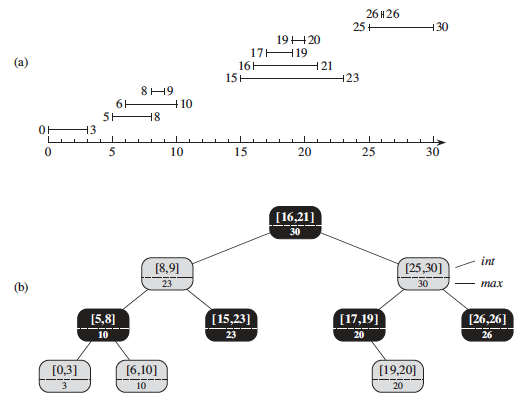
\includegraphics[scale=0.75]{interval_tree}
    \centering
    \caption {a) Intervals arranged on the number line. b)An Interval Tree constructed from the same intervals. Each node contains an interval and the maximum value of any interval in the subtree rooted at that node.\autocite{cormen2009introduction}.}
    \label{fig:interval_tree}
\end{figure}

Invocation of $callDeletions()$ uses the data accumulated by $addReadPair()$ to perform the actual deletion calling. The calling proceeds as follows:

\begin{enumerate}
    \item For each read pair determine the center point of the interval spanned by the pair.
    \item Using pair centers perform Kernel Density Estimation\autocites{rosenblatt1956remarks}{parzen1962estimation} to estimate the distribution of the location of pair centers.
    \item Using the estimated density detect regions with local maxima (clusters) that become locations for putative deletions.
    \item Using the sites of putative deletions query the Interval Tree for a list of reads that overlaps each site.
    \item For each site and set of read overlaps call the deletion boundary to be the maximal interval that is spanned by the inner distance (see Fig. \ref{fig:insert_size}) of all overlapping read pairs.
    \item Based on the width of the deletion remove all overlapping reads whose inferred insert size is greater than $deletion\_width + insert\_size\_threshold$.
    \item Output a deletion if the number of supporting reads after filtering above is $> min\_read\_support$.
\end{enumerate}

 The key approach used in this method for the clustering of read pair interval centers is Kernel Density Estimation. This approach has been used as a highly successful and efficient one-dimensional clustering method in a variety of settings\autocites{hartigan1975clustering}{kriegel2011density}{cuevas2001cluster}, but has not been applied in the context of genomic variant calling to date. 

 If we have a one-dimensional data set of iid observations $(x_1, x_2, ..., x_n)$ from some unknown distribution and we wish to estimate the pdf $f$ we can do so using:  

 $\widehat{f}_h(x) = \frac{1}{n}\sum_{i=1}^n K_h (x - x_i) = \frac{1}{nh} \sum_{i=1}^n K\Big(\frac{x-x_i}{h}\Big)$
 
 Here $K$ is a non-negative real-valued integrable windowing function, and $h$ is a smoothing parameter called bandwidth. A variety of kernels are possible. In this method we use the gaussian kernel as a way to attenuate the influence of each read pair center with distance from that center.

 \begin{figure}[H]
    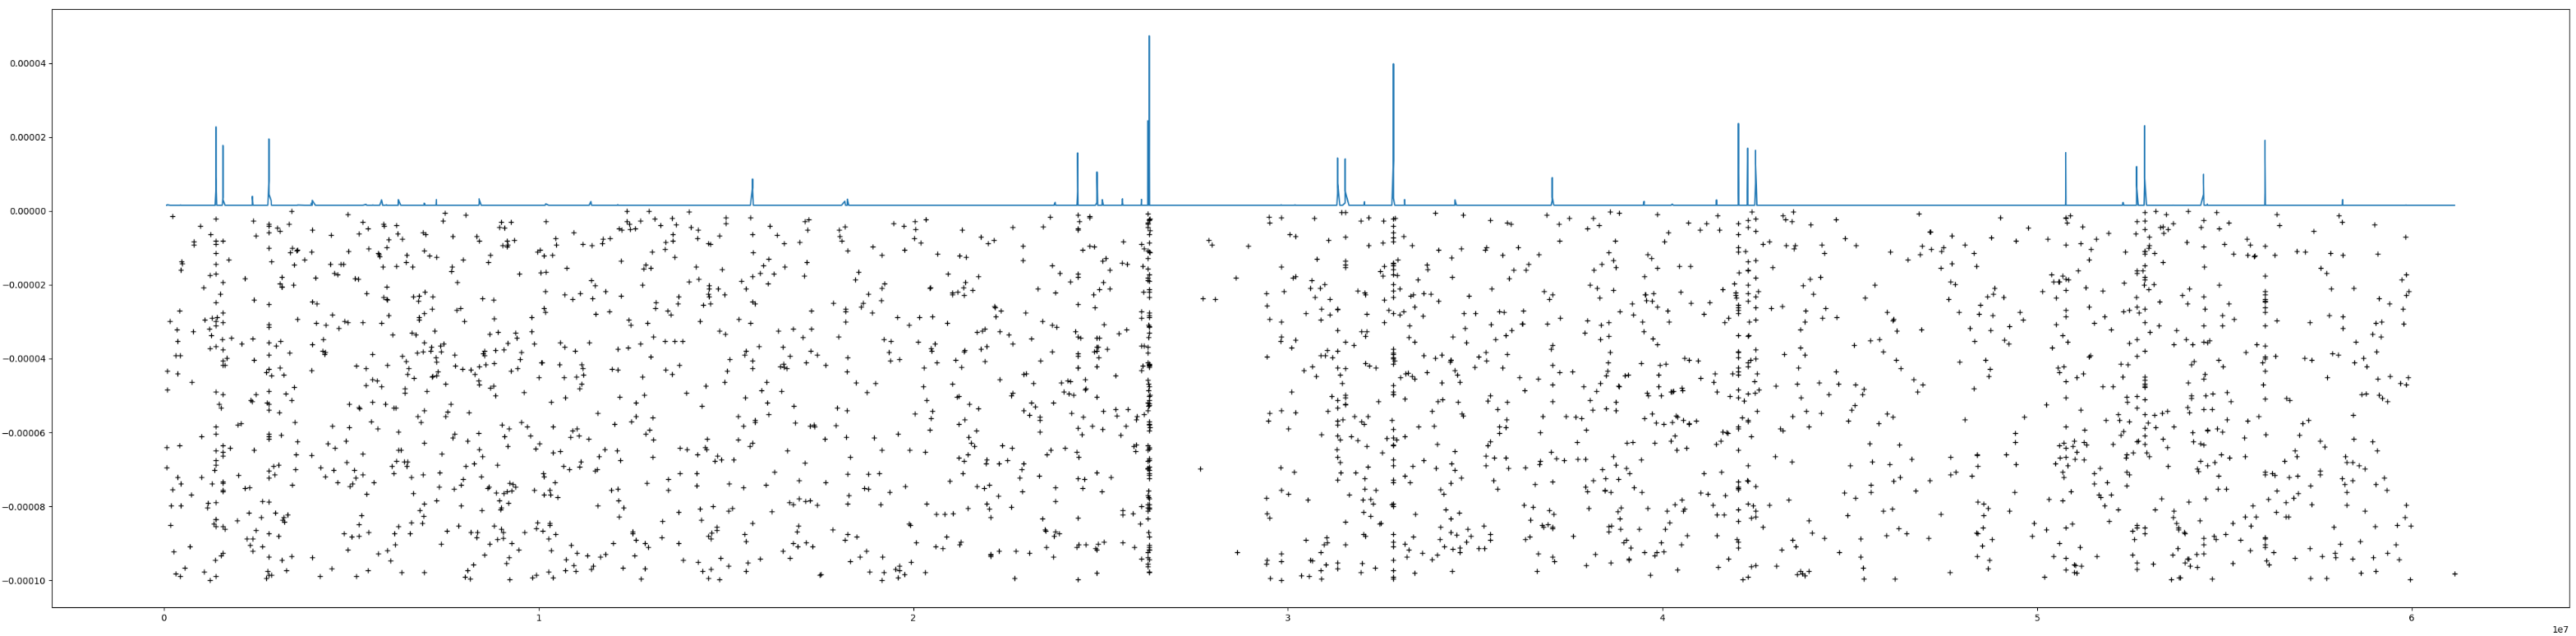
\includegraphics[scale=0.27]{kde}
    \centering
    \caption {Centers of discordantly mapped read pairs on Chromosome 20 of NA12878 (plotted as points below x-axis) along with the KDE estimate plotted above x-axis.}
    \label{fig:kde}
\end{figure}

In Figure \ref{fig:kde} we demonstrate the results of applying KDE with a gaussian kernel and a bandwidth of 100 on the 2663 discordantly mapped read pairs from Chromosome 20 of the NA12878 sample, sequenced by the Genome In A Bottle\autocite{zook2018reproducible} consortium and processed by Rheos. The x-axis specifies integer genomic coordinates from 0 to \~$6.3\times10^7$ and the y-axis is real-valued. Each point below the x-axis represents the coordinates of a centre for a single read-pair. The y-axis values for each point are randomly generated from a small interval in order to obtain visual point separation on the graph. The graph above the x-axis shows the estimated density function based on the 2663 points, with peaks indicating the position of clusters, and hence, the location of putative deleted regions. The location of peaks is obtained via a peak finding algorithm that returns the maximum value in an n-neighbourhood of points.

Once the location of the center points of putative deletions is known it is important to determine deletion size and evaluate the amount of support that exists for each deletion call. To achieve this $callDeletions()$ makes use of the Interval Tree data structure that has been constructed from all of the read pairs. The Interval Tree is queried for all read pairs that overlap the position of a given deletion center. This query is answered in $\mathcal{O}(\log{}n + m)$ time. 

\begin{figure}[H]
    
\includegraphics[scale=0.45]{deletion_read_cluster}
    \centering
    \caption {A cluster of reads spanning a germline deletion.}
    \label{fig:deletion_read_cluster}
\end{figure}

Given a set of read pairs $R = \{(r_1,r_2) : r=(r.pos, r.end)\}$ spanning the site of the deletion we are interested in determining the extent (position, and size) of the deletion. We take the deletion site (see Figure \ref{fig:deletion_read_cluster}) to be an interval $[\max_{r_{1,i} \in R}{(r_{1,i}.end)}, \min_{r_{2,i} \in R}{(r_{2,i}.pos)}]$, based on the following argument. If the deletion is homozygous, then no read in the sample should map into the deletion sequence, thus the deletion should be entirely contained in the inner distance between reads spanning the deletion. If the deletion is heterozygous, then the reads that are discordantly mapped come from the haplotype with the deleted allele, and should thus, also not have any sequence map into the deletion, again containing the deletion entirely in the inner distance between reads. Thus, the deletion boundaries are in the interval between the largest end coordinate for a read to the left of the deletion center, and the smallest start coordinate to the right of the deletion center.

Given the location and width of a putative deletion it is necessary to determine whether the deletion has sufficient support in the reads to be considered real, or may be dismissed as spurious. Many filtering strategies are possible, but the simplest relies on counting the number of read pairs that support a deletion and only retaining those that exceed a minimum threshold of $min\_read\_support$ supplied by the user. To reduce the number of false positive results we would like to remove remove from the list of reads supporting a deletion call those that are likely spurious. Since, low quality reads are already filtered by the Insert Size Filtering Service one of the few remaining sources of false positive signal are reads for which the inferred insert size is much larger than the actual deletion call that they span. These reads are either part of another, much larger, deletion, in which case they are accounted for in that deletion call, or they are spuriously mapped, as there is no other plausible reason for their large insert size. We thus, use a thresholding cutoff $insert\_size\_threshold$, supplied by the user, such that read pairs with $insert\_size > deletion\_width + insert\_size\_threshold$ are removed from the list of reads supporting a particular call. Afterwards, deletions that have read support exceeding the $min\_read\_support$ threshold are selected as called variants. 

The variant quality for the deletion is taken to be $vqual = \sum_{r \in R}{r.mapq}$ i.e. the Phred-scaled probability that all of the reads that support the deletion have been mis-mapped. All of the variants that have been called are emitted in the Insert Size Clustering Service's output stream in the format $M_{del} = \{m_i: m_i = (header, payload)\}$ where $m.payload = V = \{v_i: v_i = (s\_id, contig, pos, length, vqual, R)\}$, as described in Table \ref{tab:op_insert_size_clustering}, where the header includes the query details that are being answered.


\section{Rheos implementation}

In order to prove the viability of the concepts behind Rheos we have built and tested a limited implementation of Rheos. This implementation provides a data streaming architecture of services and is able to perform genome alignment, followed by online germline SNP and deletion calling, as described in Section \ref{sec:main_body_domain_specific_problems}. The source code is available on github at - https://github.com/llevar/rheos. In this section we describe the details of the technical implementation, including the key approaches taken for the establishment of data streaming, service organization, scalable deployment, and performance optimization. Even though the implementation is fully functional and has been used to analyze real data, it is worth noting that due to the extremely broad scope of the overall Rheos framework, and the limited resources available, the implementation focuses on a narrow set of use cases and is meant to be treated as a proof of concept rather than a production system.

As in the implementation of Butler (see Chapters \ref{ch:butler_architecture}, \ref{ch:butler_implementation}) we make a concentrated effort to rely on established Open Source software frameworks where possible to ensure that components of Rheos are robust and scalable, require minimal maintenance, and can be easily deployed on a variety of platforms. Some of the key frameworks used by Rheos are Apache Kafka, Google Kubernetes, Docker, and Prometheus.

The implementation is focused on the following key services:

\begin{description}
    \item [Read Mapping Service] - Reads a FASTQ file and turns it into a set of streams for mapped and unmapped reads and read-pairs.
    \item [Locus Processor Service] - Reads a stream of mapped read pairs and incorporates variant evidence from the reads into a model of genomic Loci. Emits a stream of updated Loci.
    \item [Locus Saver Service] - Reads a stream of Loci and stores them in a distributed data store.
    \item [Variant Calling Service] - Reads Loci from a data store and performs germline SNP calling. Emits a VCF file.
    \item [Insert Size Filtering Service] - Reads a stream of mapped read pairs and emits a stream of filtered high quality read pairs that are discordantly mapped and can be used for calling deletions.
    \item [Insert Size Clustering Service] - Reads a stream of discordantly mapped read pairs and calls germline deletions via KDE clustering. Emits a stream of deletion variants.
\end{description}

We first focus on the general architecture of a Rheos service and describe how services communicate with each other, then describe the deployment and operation of the Rheos system as a whole, and finally describe the individual services to comprise the Rheos implementation.

\subsection{Rheos Service}
A service in Rheos is a continuously running program with a well defined interface (implementing one or more operations described in Section \ref{sec:rheos_data_streaming_model}), and a set of well understood operating characteristics. Even though a service author is completely free to use different technologies for different services (as long as the interface is respected), we have chosen to implement the initial set of Rheos services in Python. Since Rheos services are typically streaming services, their operations are most often invoked automatically when new data appears on the stream.

\begin{figure}[H]
    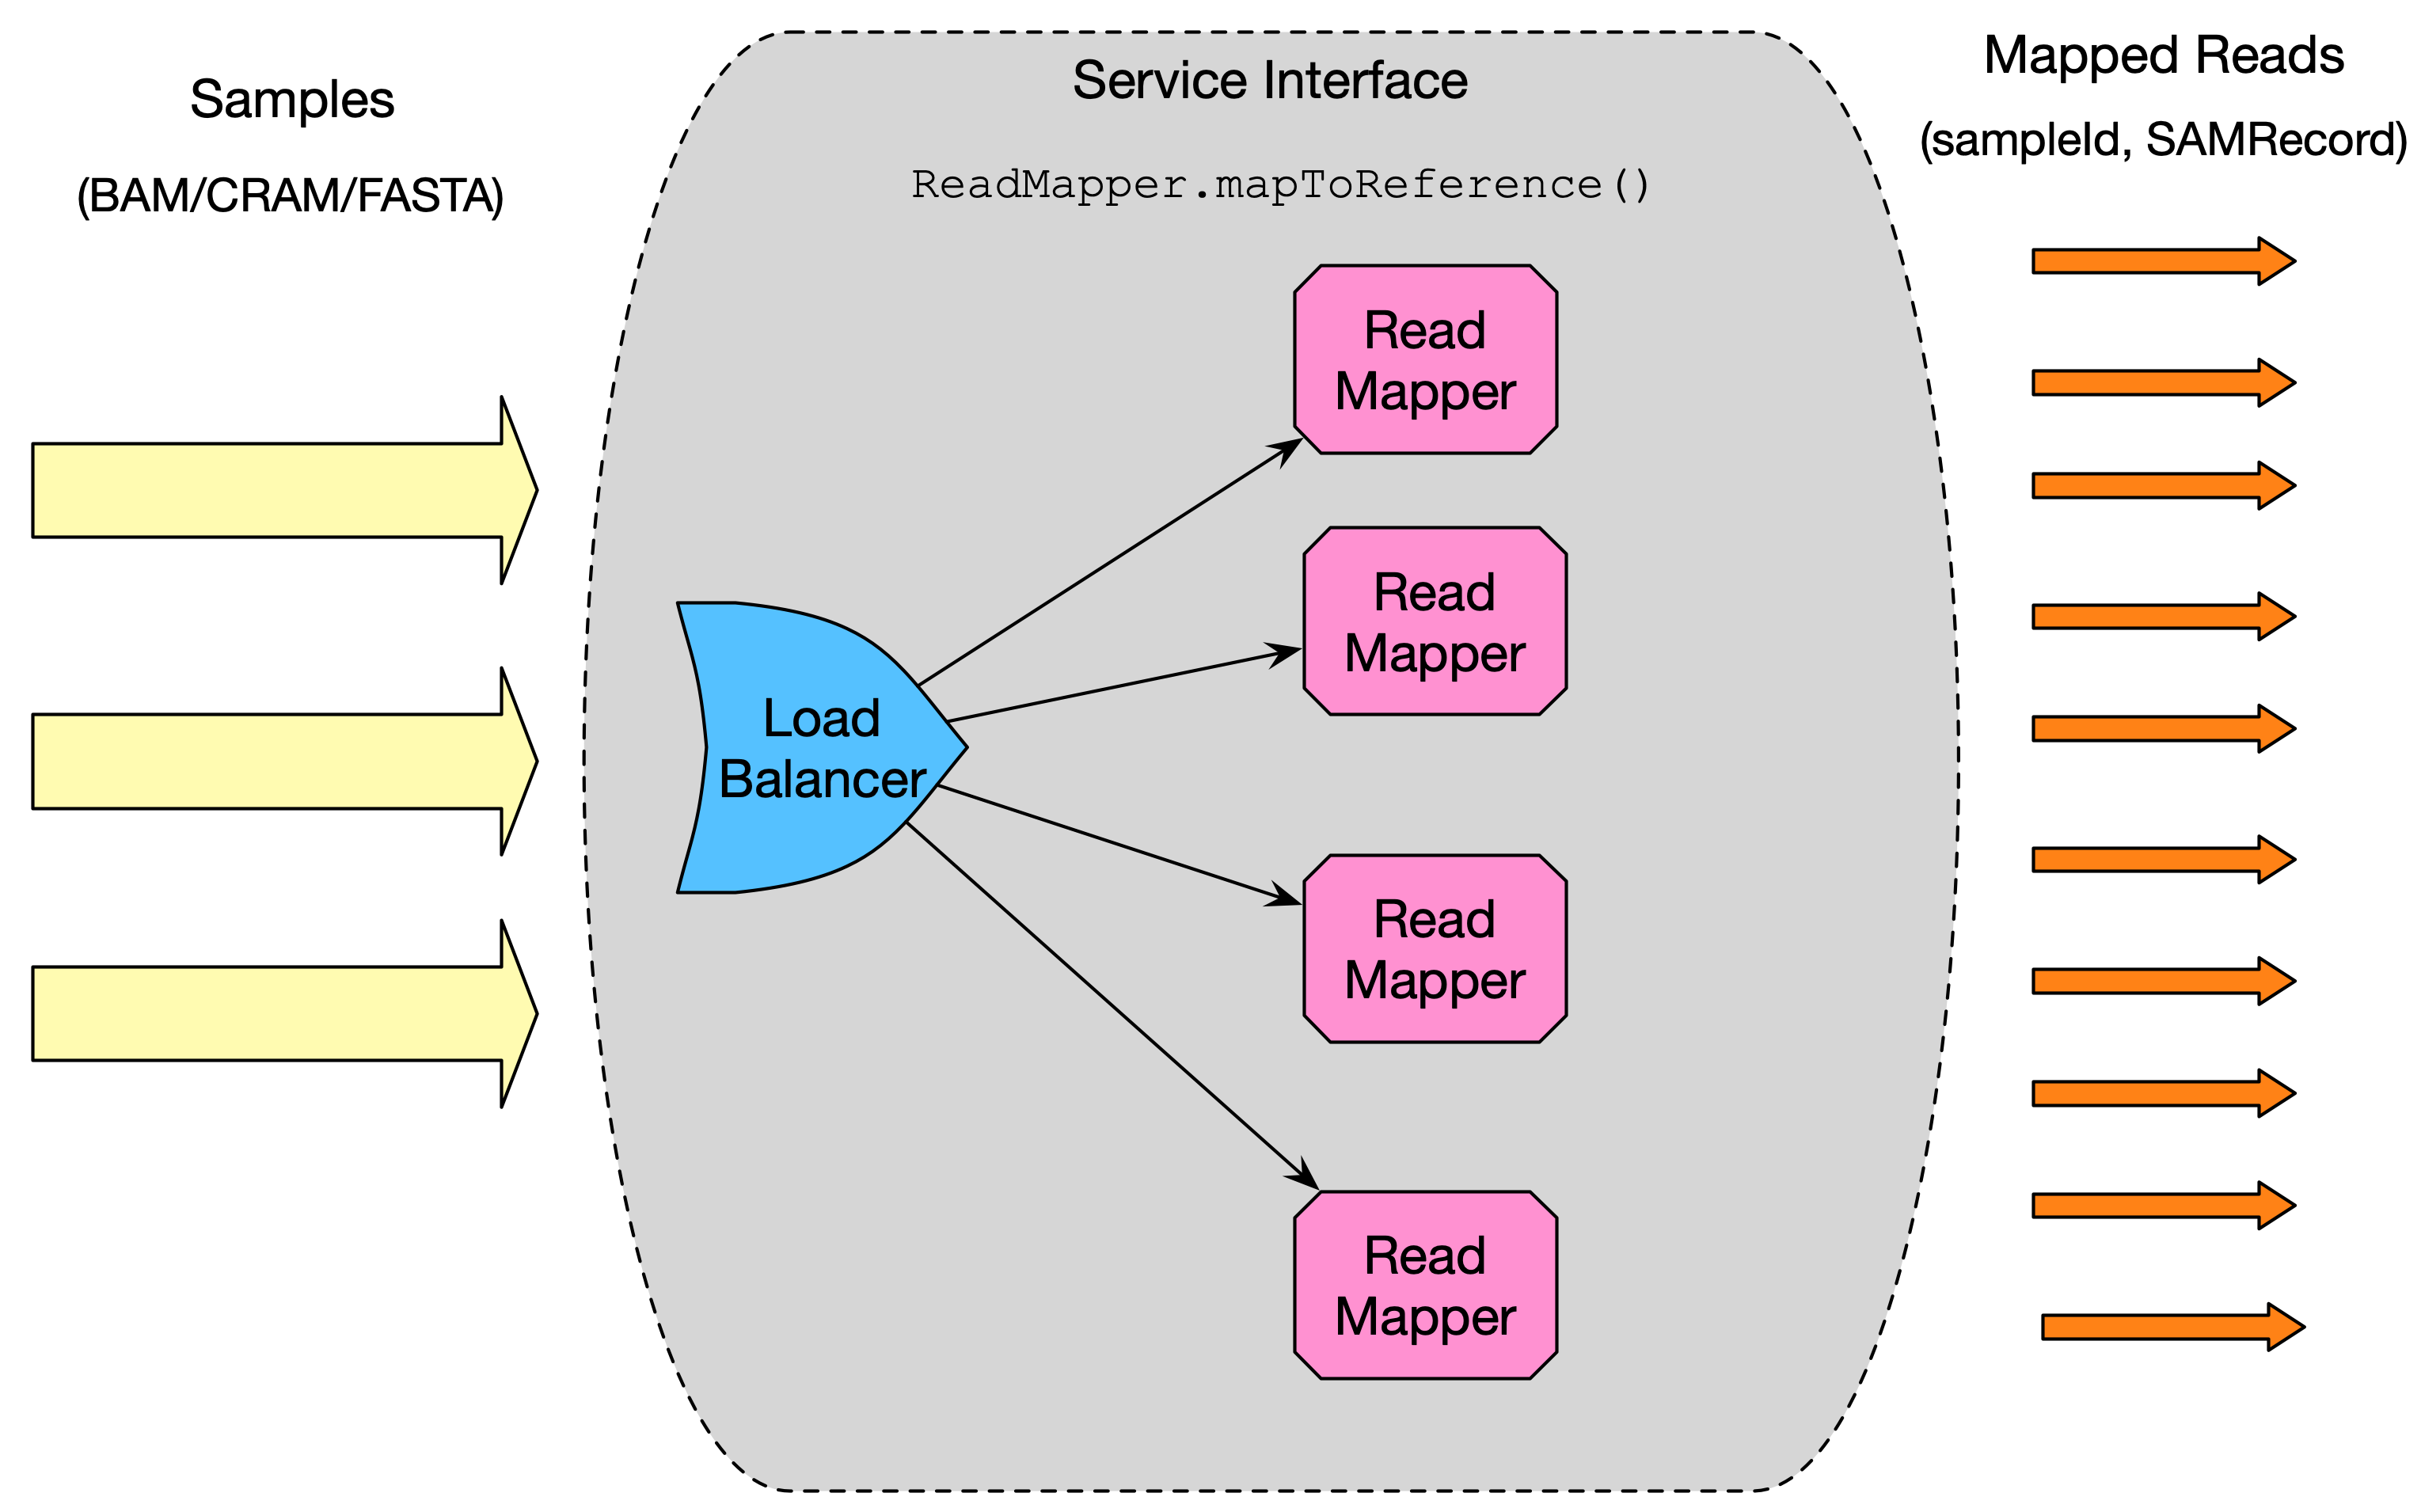
\includegraphics[scale=0.55]{rheos_service_interface}
    \centering
    \caption {Several instances of the Read Mapping Service are managed behind a Load Balancer.}
    \label{fig:rheos_service_interface}
\end{figure}

Figure \ref{fig:rheos_service_interface} demonstrates several key concepts behind Rheos services using the example of a Read Mapping Service:

\begin{itemize}
    \item The service transforms the granularity of the data from sample-level on the input to read-level on the output. 
    \item The service implements a streaming operation of type Decorator, it decorates the incoming read data with additional information, that of the read coordinates, CIGAR string, mapping quality, etc. 
    \item The service provides a uniform interface to its clients, that of \emph{ReadService.mapToReference()}. Machines that implement this interface are indistinguishable from each other. 
    \item Clients of the service talk to the service interface through the Load Balancer. The DNS entry for the service returns the IP of the Load Balancer which is then responsible for routing requests to one of the service instances. This allows one to control the scalability of the service, seamlessly adding and removing instances of the Read Mapper depending on the rate of the data that is coming into the system, and the ability of downstream services to process it.  
\end{itemize}

When services are deployed it is desirable to be able to easily deploy them to a variety of different environments and achieve a level of resource and environment isolation, so that other programs running on the same machine can only minimally impact the installation and running of the service. To accomplish these goals, all of the services in Rheos follow a containerized approach using Docker\autocite{merkel2014docker}.

\begin{figure}[H]
    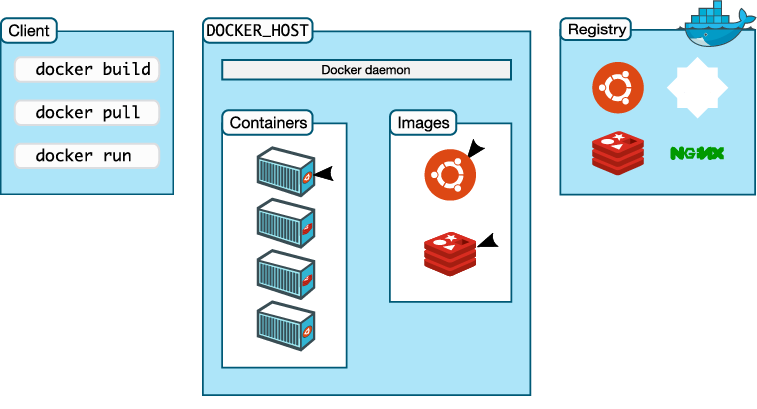
\includegraphics[scale=0.55]{docker_architecture}
    \centering
    \caption {Docker system architecture (https://docs.docker.com/engine/docker-overview/).}
    \label{fig:docker_architecture}
\end{figure}

Docker is an Open Source framework that isolates the execution of a program from the host machine and other programs by encapsulating it in a lightweight Linux container. The container is a separate instance of an operating system and a program running inside it is not aware of its enclosing environment. The Docker architecture consists of three main components (see Figure \ref{fig:docker_architecture}). A machine that can run Docker containers (the Docker Host)
needs to be running the Docker Daemon. A container is a runtime instance of a Docker environment, but the blueprint from which all containers are created is called a Docker Image. The user starts with a base image that only has an operating system in it. The user can then augment the image by installing additional software packages and custom programs. This can be done interactively inside a shell inside a running container, or declaratively via a Dockerfile. When the user is finished preparing their image they can use the Docker Client to build it and upload it to an external Docker Registry. This is an external registry where various Docker images are hosted. When Docker Daemon needs to create a container it pulls down the requisite image from a registry to the local machine, and then instantiates the container. Containers can be started and stopped, created and deleted easily, and provide a great deal of abstraction and simplification when it comes to running many different applications, with potentially conflicting dependencies on a server. They also provide a seamless migration path from the local development machine, through the testing environment,and into production. All Rheos services are implemented to be encapsulated inside Docker containers.

\begin{figure}[H]
    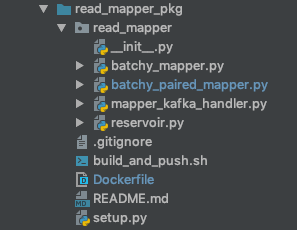
\includegraphics[scale=1]{rheos_service_file_structure}
    \centering
    \caption {Rheos service file structure.}
    \label{fig:rheos_service_file_structure}
\end{figure}

The layout of a Rheos service file structure is standard (see Fig. \ref{fig:rheos_service_file_structure}). One or more Python files implement the service functionality in the form of a Python module. The file \emph{setup.py} provides a list of dependencies that are needed for the functionality of the service. The \emph{Dockerfile} specifies how to build a Docker image of the service (See Listing \ref{lst:rheos_dockerfile}). 

\captionof{listing}{Example Dockerfile for setting up a service. \label{lst:rheos_dockerfile}}
\begin{minted}
[
breaklines=true,
linenos,
fontsize=\footnotesize,
frame=lines,
framesep=2mm,
baselinestretch=1.2
]
{shell}
FROM python:3.7.2-alpine3.8
RUN apk add --no-cache build-base python3-dev zlib-dev cython make bzip2-dev xz-dev libcurl
WORKDIR /app
COPY . /app/
RUN python setup.py install
RUN mkdir /app/log && touch /app/log/mapper.log
ENTRYPOINT ["python", "read_mapper/batchy_mapper.py"]
\end{minted}

The Dockerfile uses a base image of Alpine Linux with python 3.7.2 preinstalled. Several addon linux packages are installed. The service module code is copied to the \mintinline{shell}{/app} directory. \mintinline{shell}{setup.py} is run to install all of the service's dependencies, and the program entrypoint for the Docker container is set to point to the service executable.

The file \mintinline{shell}{build_and_push.sh} is a shell script that is responsible for building a Docker image using the supplied Dockerfile and pushing this image to a Docker registry (hub.docker.com). Any deployment of the service can now pull down this image from the registry and instantiate new containers from it.

As there is a good deal of functionality that is common between several Rheos services there is a separate Python module called \mintinline{shell}{rheos-common} that houses both utility classes and commonly used models (such as that for genomic loci) in its submodules. This module is hosted on Pypi and can be installed from anywhere using standard Python installation techniques such as \emph{pip}.

The wire format for messages exchanged between services is currently schema-less and relies on standard Python serialization mechanisms (namely \emph{pickle}), and \emph{json}. Although \emph{json} is completely generic, \emph{pickle} is proprietary to Python and thus represents a weakness of the current implementation. A generic wire format with a defined schema will be a future improvement.

Serialized messages are streamed between services via distributed queues.


\subsection{Queueing}

For message queueing Rheos relies on an Open Source framework called Apache Kafka\autocite{kreps2011kafka}. Kafka queues provide a distributed fault-tolerant implementation of the publish/subscribe mechanism, and streaming. 

\begin{figure}[H]
    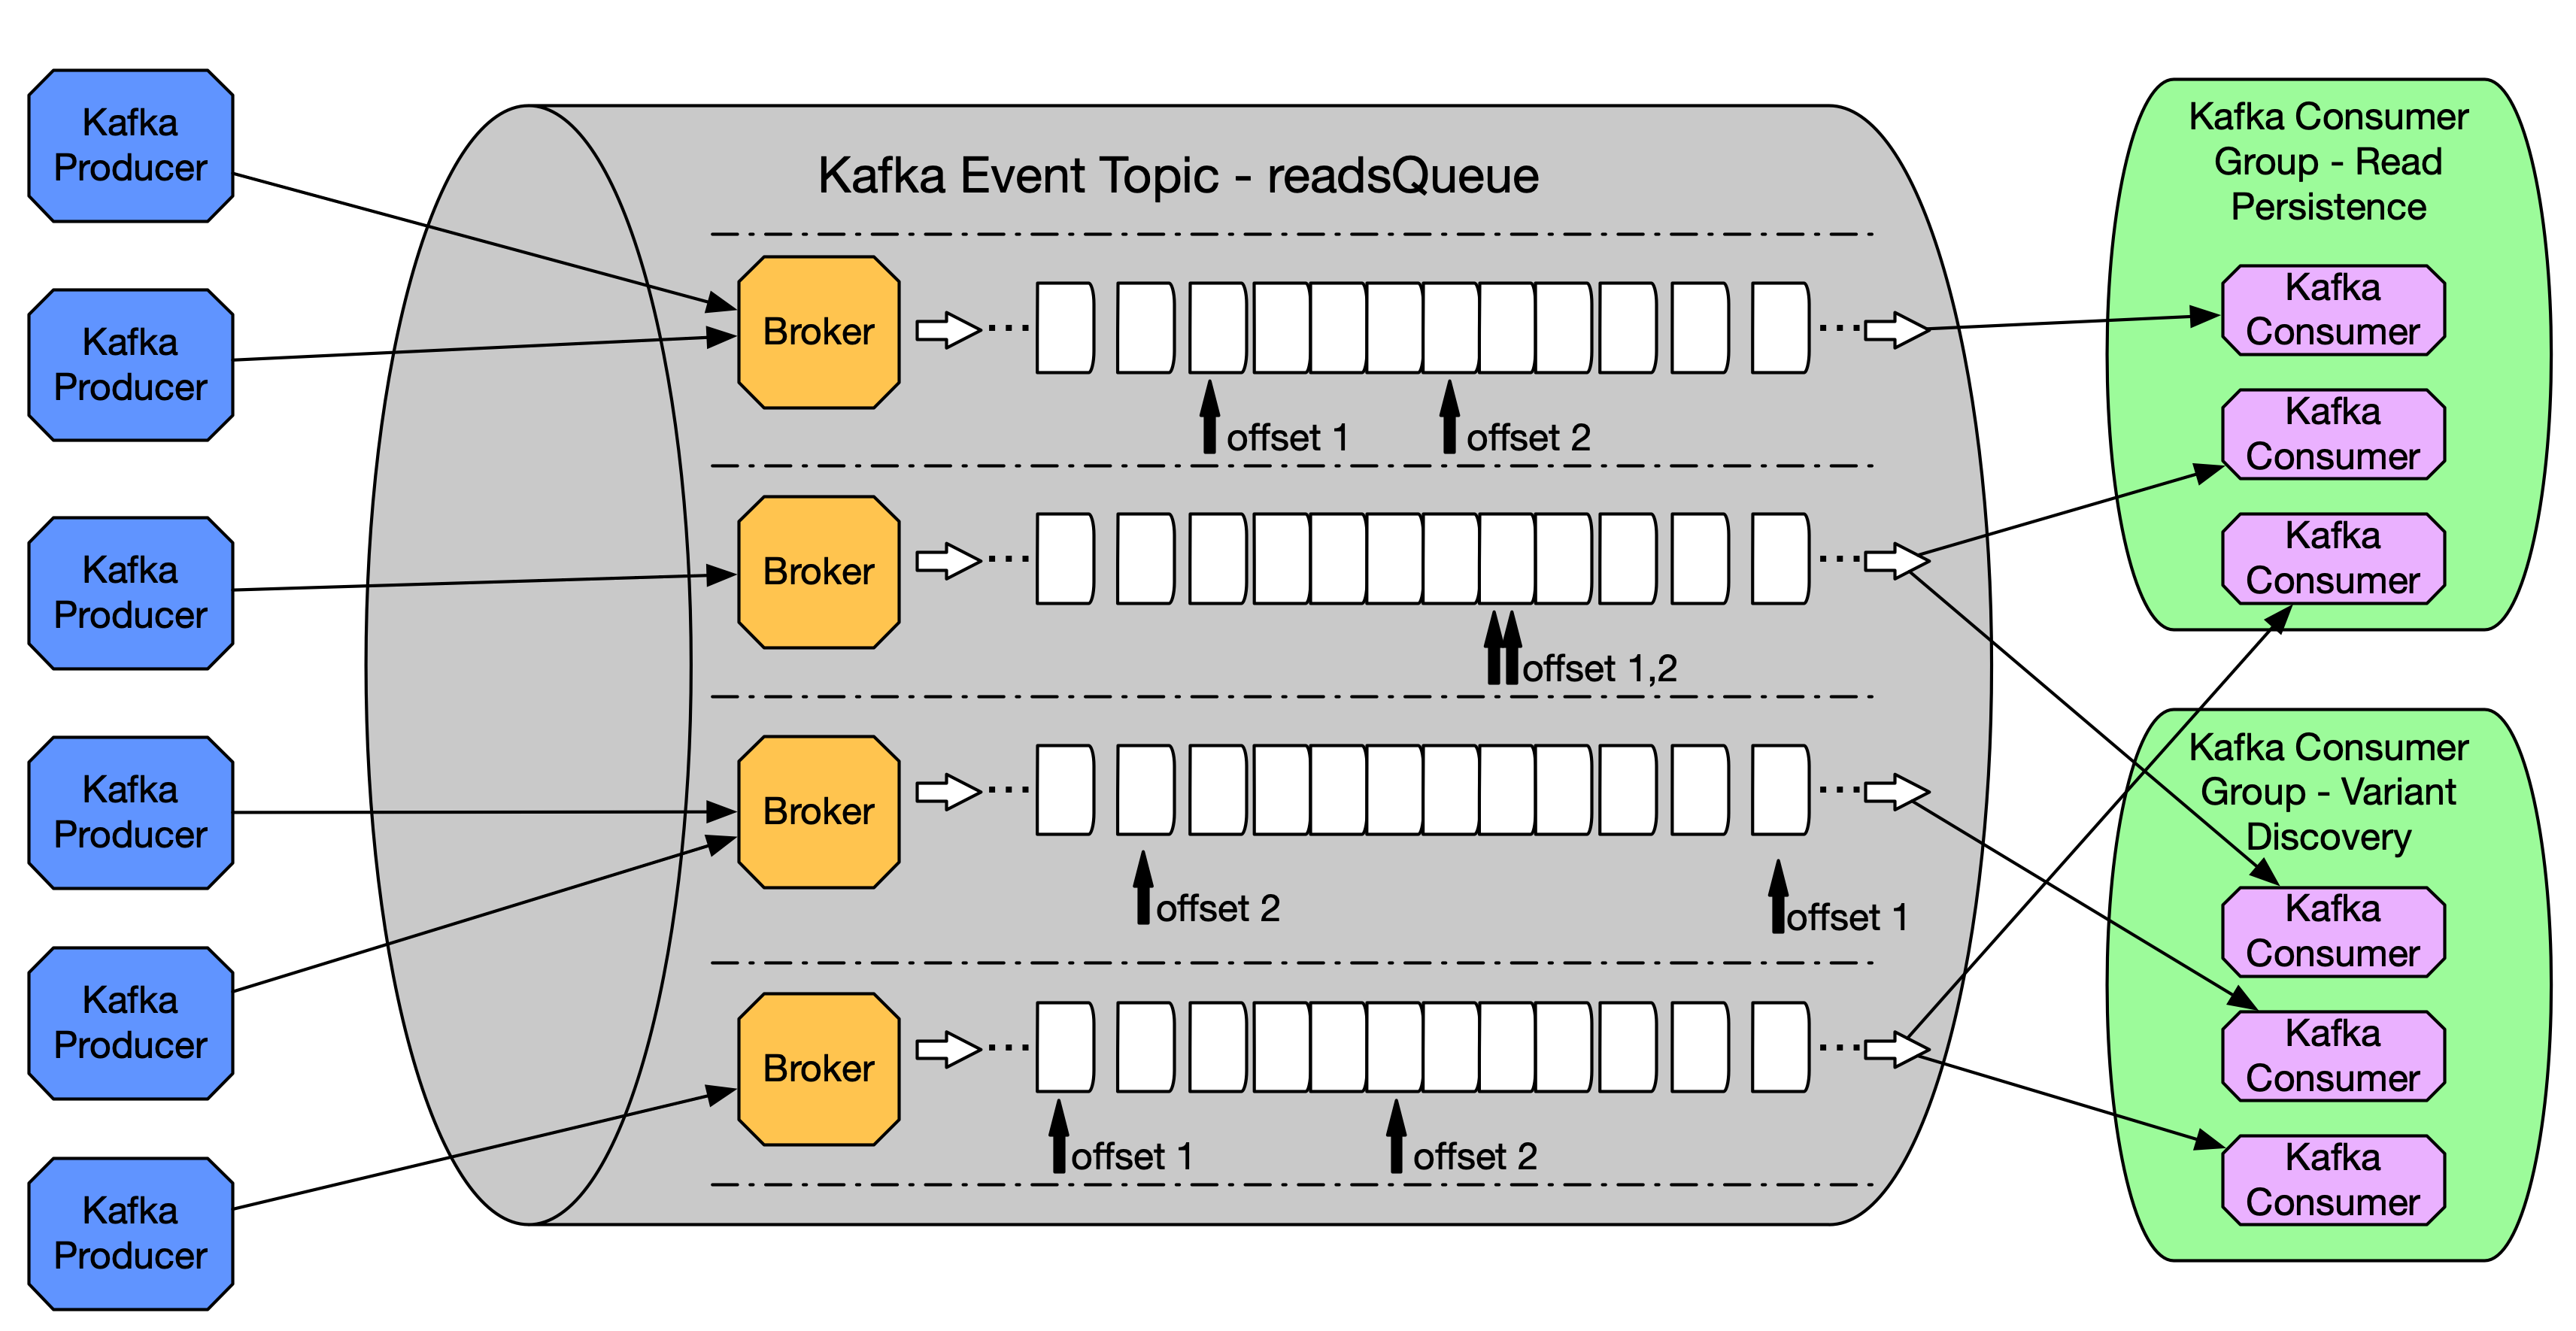
\includegraphics[scale=0.48]{kafka_queue}
    \centering
    \caption {Example of a Kafka queue with multiple data producers and consumers.}
    \label{fig:kafka_queue}
\end{figure}

At the heart of Kafka lies an Event Topic (see Figure \ref{fig:kafka_queue}). The topic is a distributed transaction log. When messages are put in the queue, they are never deleted by a consumer. Instead, consumers keep an offset into the log that tells them where they currently are in the processing of the data. Offsets can be moved freely so that a consumer may process the same message multiple times if needed. Data is deleted from the queue by virtue of a retention policy that removes data that is older than some specified time period. 

The queue is distributed between several machines by using partitions. A Kafka partition is a function that specifies how many logical and physical partitions of the data exist. Data may be partitioned onto several machines based on data size considerations, or it may be partitioned based on a logical grouping. In the former case, an automated partitioning function is employed that decides which partition to send new messages to in round-robin fashion. In the latter case a logical partitioning function needs to be supplied by the user. Rheos mainly uses the latter approach to partition data by genomic coordinate (see Section \ref{sec:main_body_partitioning} for details.)

Data producers put messages into the queue by communicating with a Broker. A Broker is a Kafka service that manages one or more queues on a particular machine. Multiple Brokers may be put in a cluster for load balancing. A data producer establishes a connection with a broker using a client library (\mintinline{shell}{kafka-python} in the case of Rheos). The partitioning function determines which machine a particular message ends up on.

On the data consumer side, consumers are organized into Consumer Groups. Each Consumer Group is a set of consumers that are assumed to be a separate entity from the consumers in all the other consumer groups. A Consumer Group has its on separate set of offsets into every partition of a topic that it is subscribed to and these do not interefer with the offsets of other groups. Assignment of consumers within a group to partitions of a topic can be automated or manual. In the case of automated assignment Kafka will decide on its own how to pair a consumer with a partition. In the case of manual assignment the partitioning function is used to make the assignment. It is in general not advisable to have multiple consumers from the same group reading data from the same partition. 

We implement a generic Kafka Handler in the \mintinline{shell}{rheods-common} module. This handler allows Rheos services to initialize Kafka producers and consumers. serialize and deserialize data using pickle and json, and to store and retrieve messages using the topics that have been set up for inter-service communication.

\subsection{Partitioning} \label{sec:main_body_partitioning}

Partitioning is important in Rheos not only because the data is quite big and thus needs to be parceled out to multiple machines, but also because data exhibits strong locality subsequent to the read mapping stage, where most of the data that is required to make decisions about the presence or absence of a genomic variant resides in some small genomic neighbourhood around the variant. It is thus natural for us to partition the read data (which is biggest in size) by genomic coordinate.

\begin{figure}[H]
    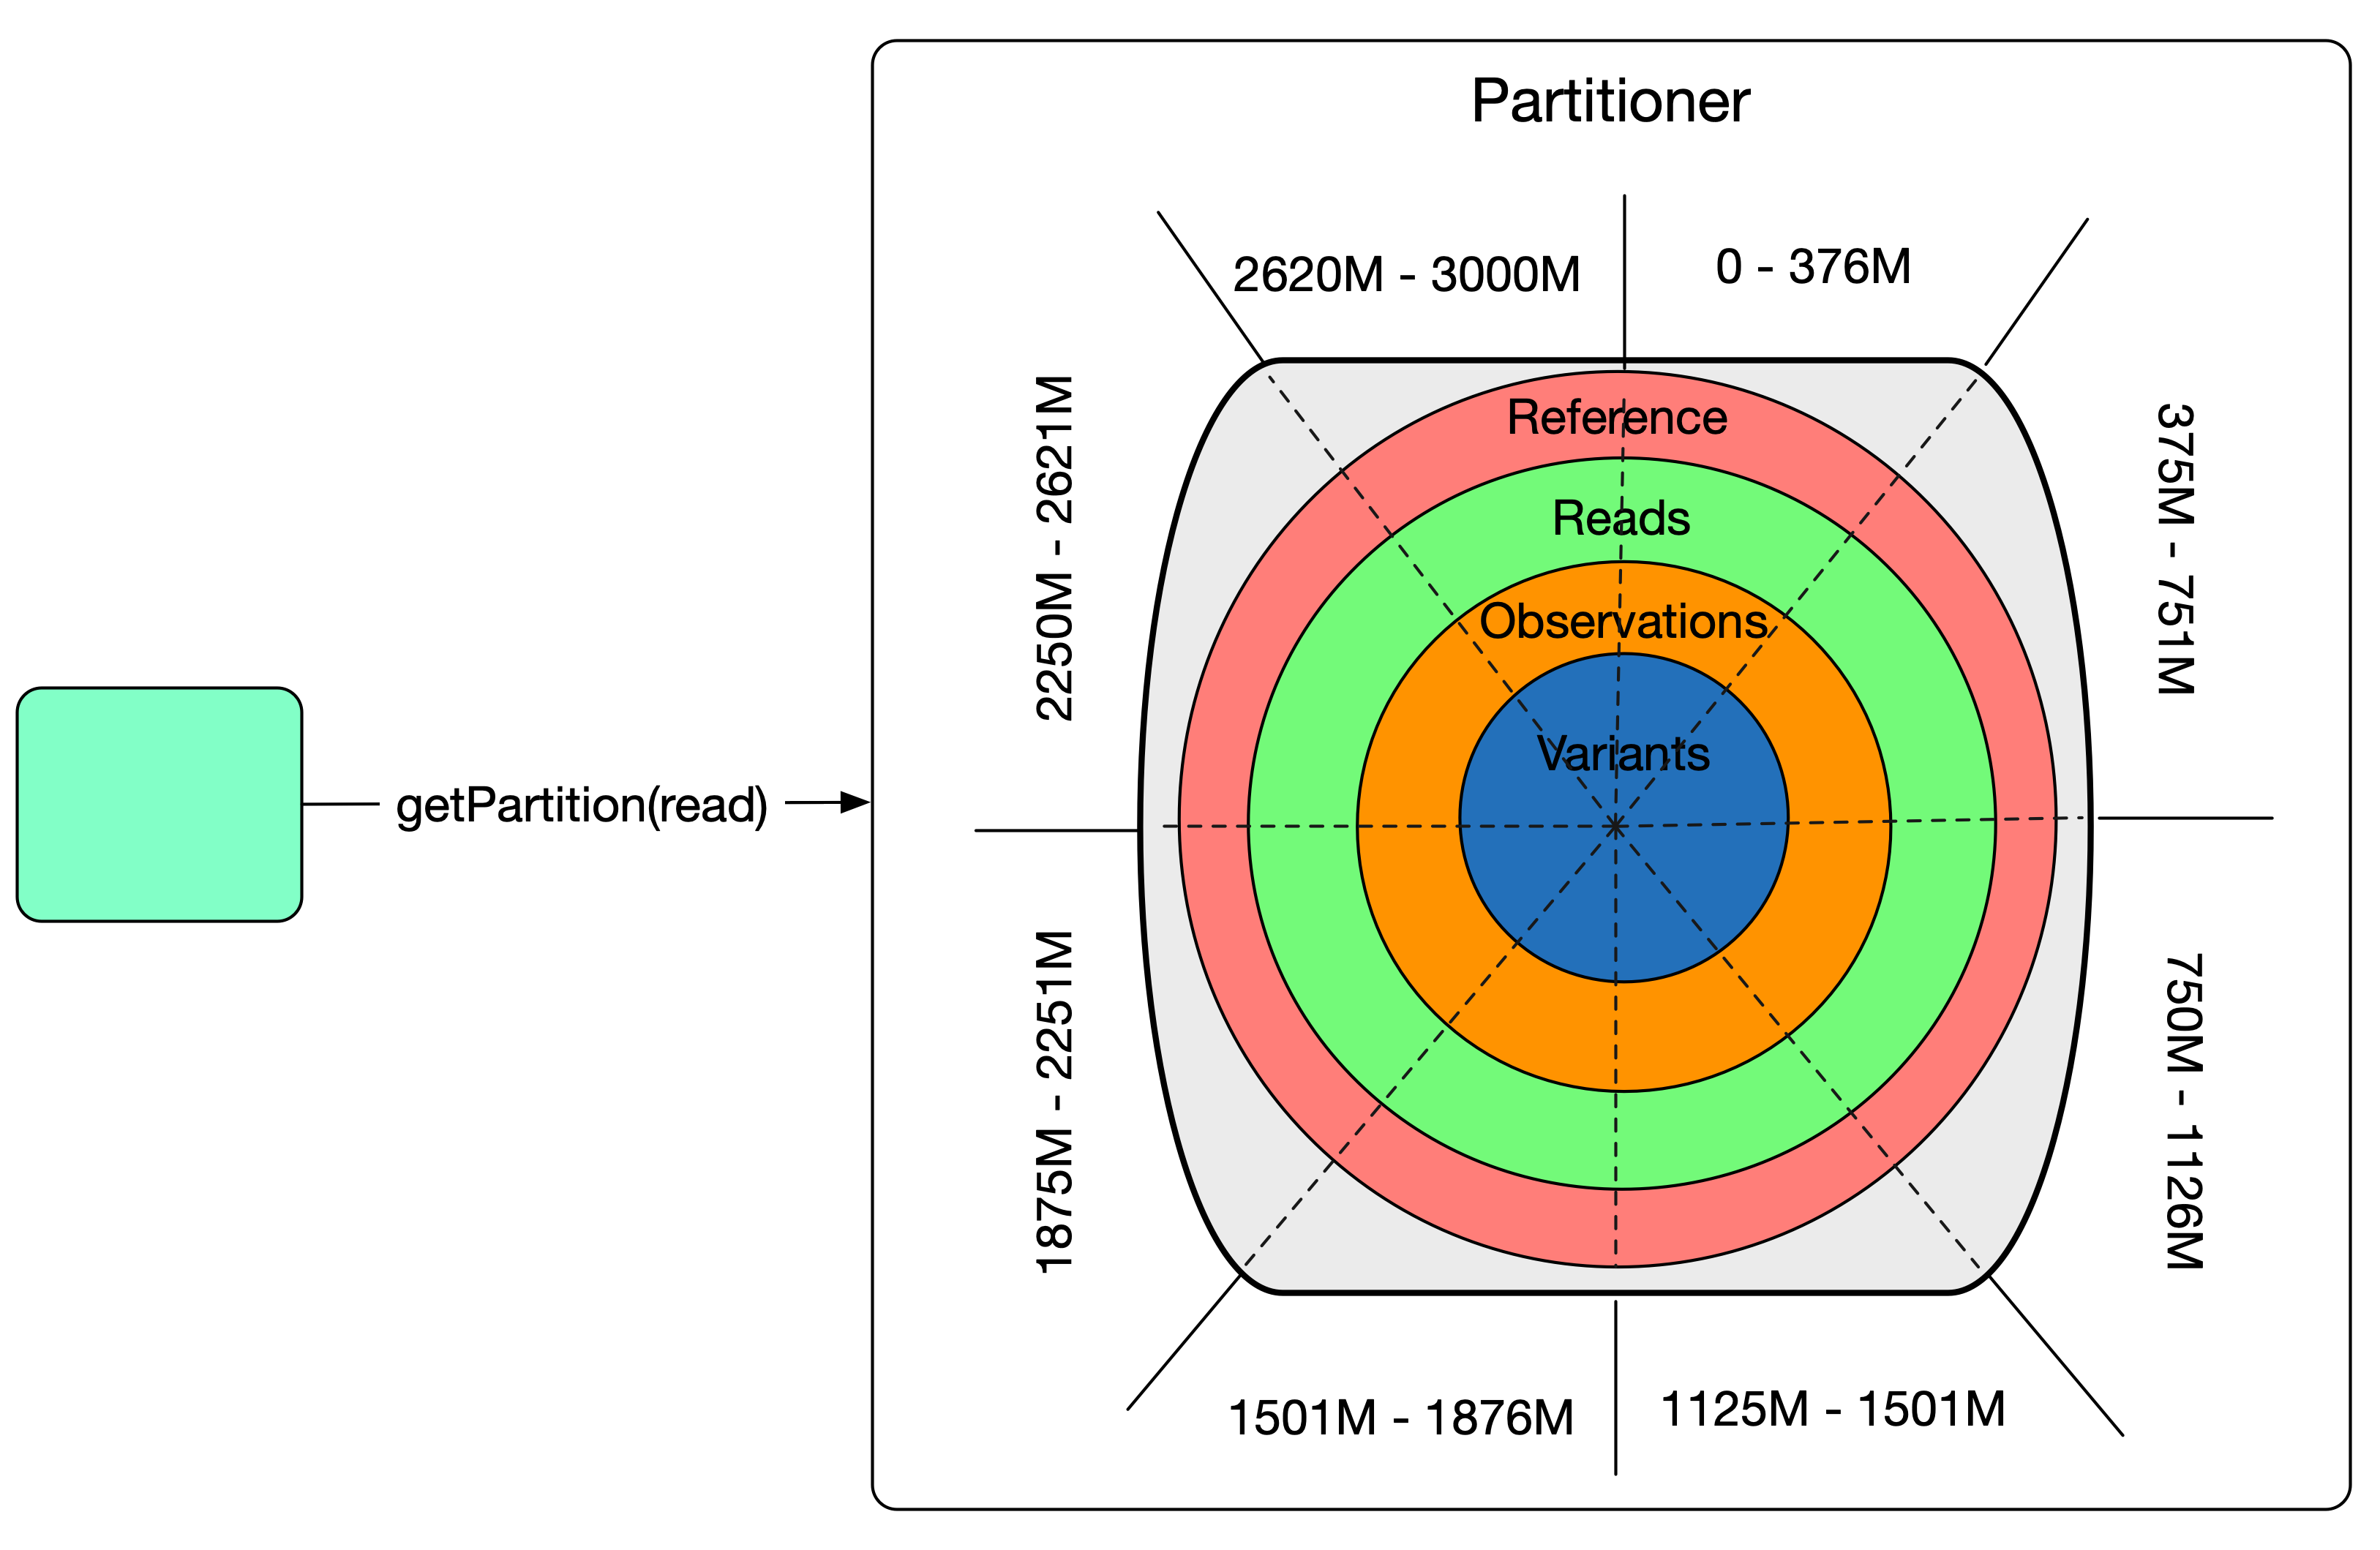
\includegraphics[scale=0.48]{rheos_data_partitioning}
    \centering
    \caption {Rheos data is partitioned by genomic coordinate.}
    \label{fig:rheos_data_partitioning}
\end{figure}

Partitioning can be challenging because different partitions end up on different machines, yet certain reads and structural variants end up spanning one or several partitions. We need to decide what to do at the partition boundaries, i.e. if a particular read ends up spanning the boundary, does it end up in one partition, the other, or both? If a read ends up in two partitions how does one avoid double counting the read in downstream processing? Likewise, if the reads supporting one breakpoint of a structural variant lie in one partition, and the reads supporting the other breakpoint lie in another partition, how can these be put together to form a single variant?

We take a simple approach in the initial Rheos implementation that will require further work when the system is elaborated. The following assumptions are made by the Partitioner:

\begin{itemize}
    \item All partitions are of equal size, except at the end of contigs.
    \item Reads that span multiple partitions are assigned to all partitions that they map to (see Figure \ref{fig:rheos_partition_boundary}).
    \item A given read will always map to the same set of partitions.
    \item All reads that are unmapped end up in the "unmapped" partition.
    \item All reads that map to special contigs (like decoy sequences) are mapped to a special "other" partition.
\end{itemize}

\begin{figure}[H]
    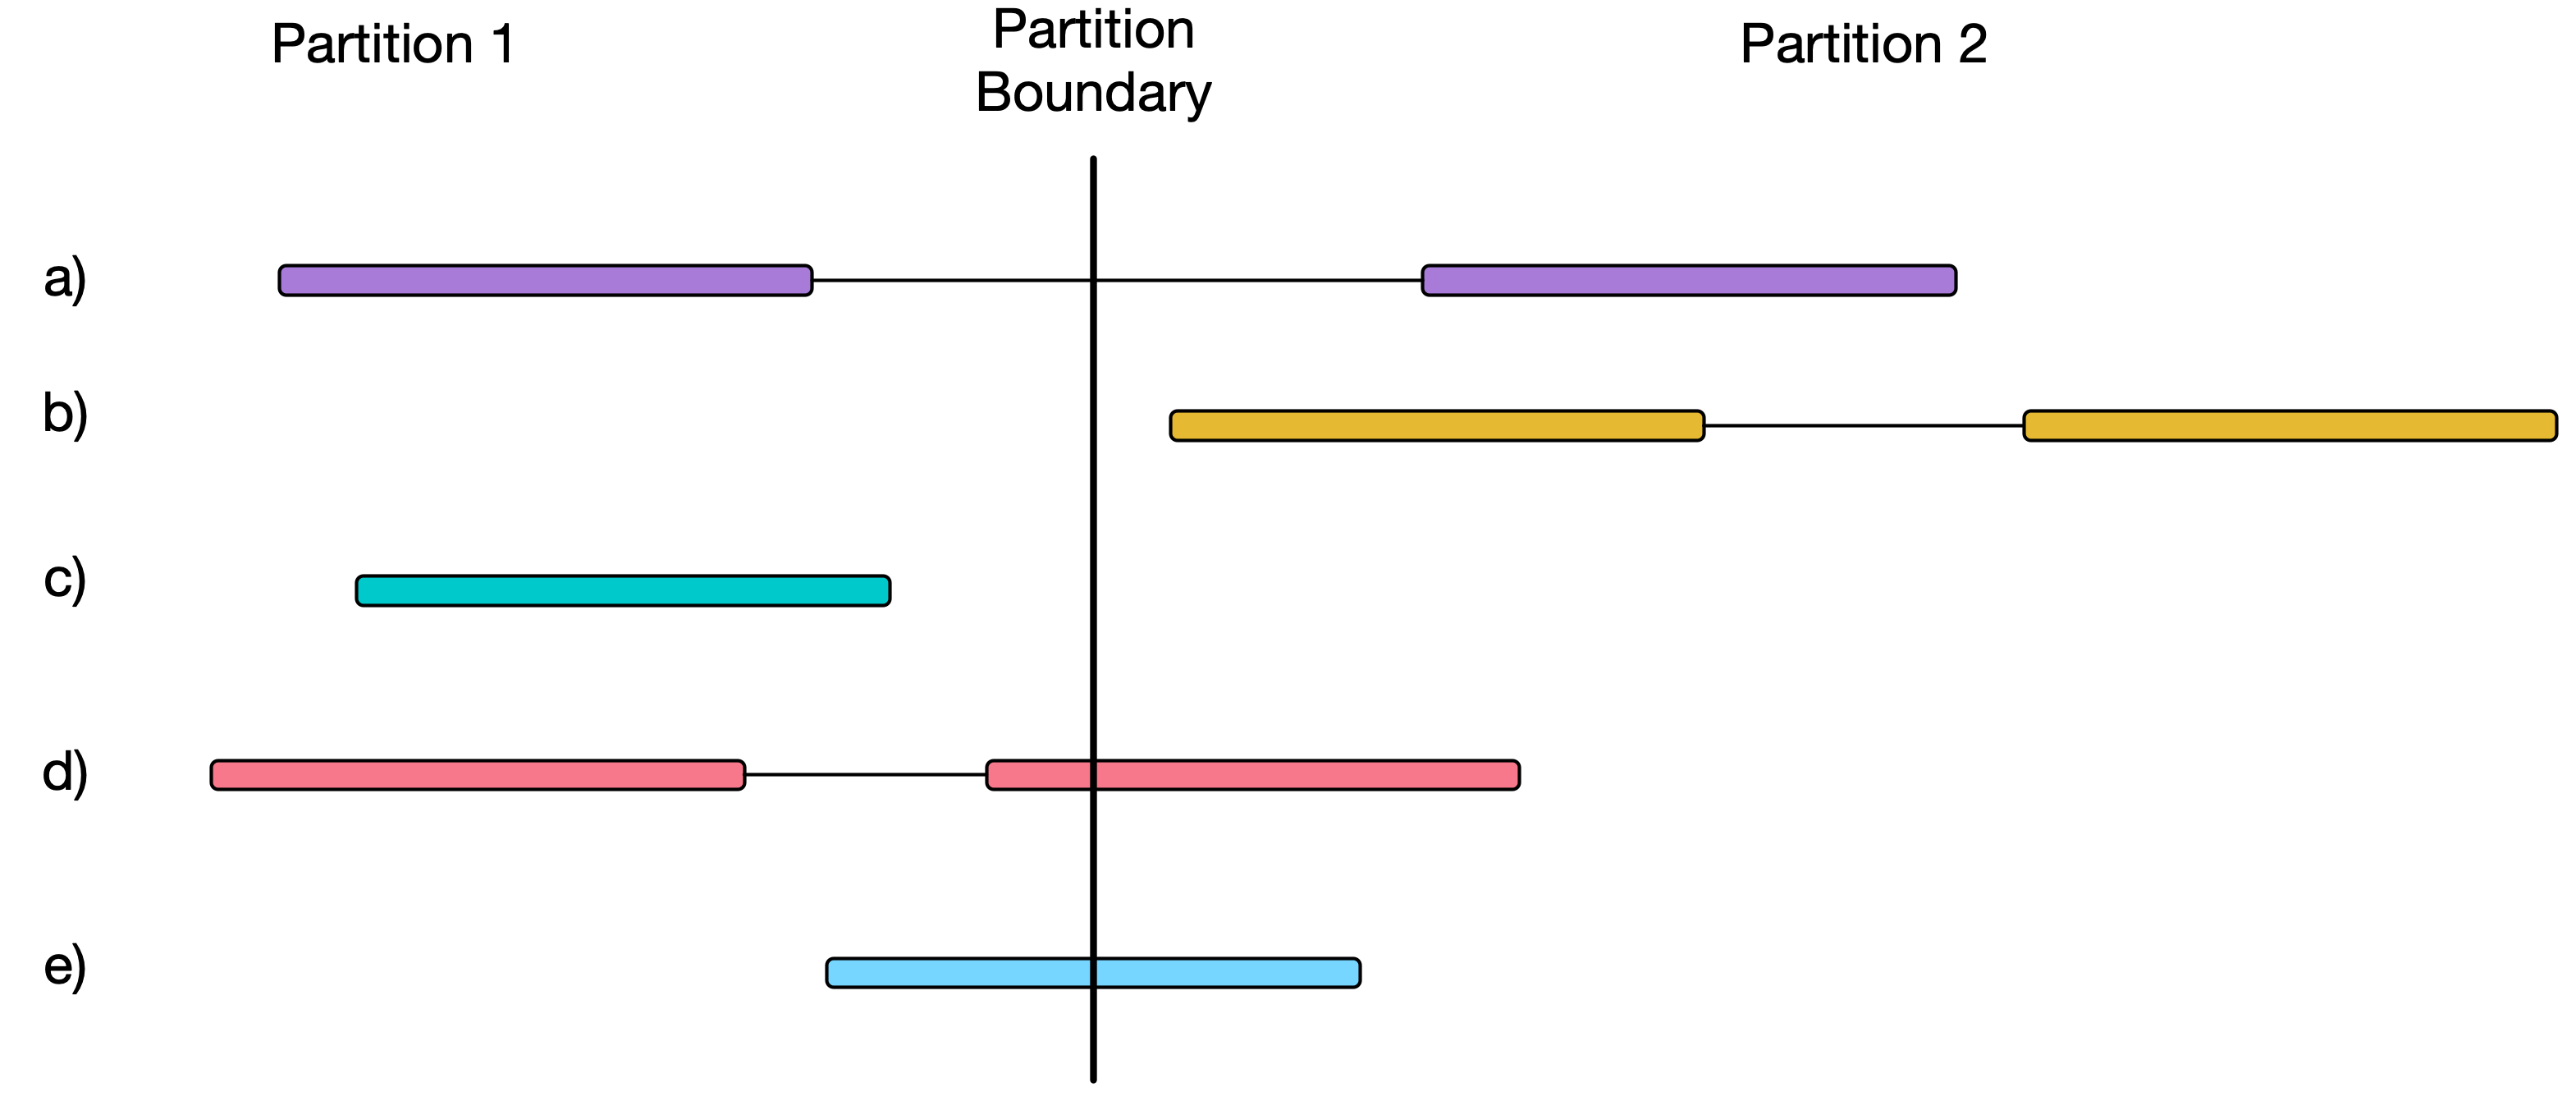
\includegraphics[scale=0.55]{rheos_partition_boundary}
    \centering
    \caption {Reads that map near the partition boundary - a) The read pair maps to partitions 1 and 2, b) The read pair maps to partition 2 only, c) The single read maps to Partition 1 only, d) The read pair maps to partitions 1 and 2, e) The single read maps to partitions 1 and 2.}
    \label{fig:rheos_partition_boundary}
\end{figure}

In general the partitioning problem can be stated as follows:

Given a reference genome $G = G_{main} \cup G_{other}$, where $G_{main} = \{g_i: g_i = (name_i, length), name_i \in \{1,..,22,X,Y,MT\}\}$ and $G_{other} = \{g_i: g_i = (name_i, length), name_i \in Aux\_Contig\_Names\}$, we assign a set of indexed partitions $P = \{(g_i.name, start, end, i) : g_i \in G_{main}, i \in [1,|G_{main}|]\} \cup \{("other",|G_{main}|+1), ("unmapped",|G_{main}|+2\}$, where given a set of reads $R = \{r_i: r_i = (contig, pos, end)\}$ (most often a read or a read pair), we desire to have a function $f:R \mapsto \mathcal{P}(P)$ (where $\mathcal{P}(P)$ is the power set of $P$) that maps those reads to a set of partitions from $P$.

We opt for partitions of fixed width $partition\_width$ (except at ends of contigs) and implement Algorithm \ref{ag:partitioner}, that, given $G$, produces $P$, and for a given interval or read pair returns a set of partitions they map to:

\begin{algorithm2e}[h!]
    \DontPrintSemicolon
    \footnotesize
    \textbf{Function} {\sc initializePartitioner}$(g\_main, g\_other, partition\_width)$
    \Begin {
        $partition\_index \gets 0$\;
        \For{$name, length $ {\bf in }$g\_main$}{
            $num\_partitions \gets $ {\sc ceiling}$(length / partition\_width)$\;
            \For{$i \gets 0 $ \KwTo $num\_partitions$}{
                $left \gets i \times partition\_width + 1 $\;
                $right \gets $ {\sc min}$((i + 1) \times partition\_width, length)$\; 

                $new\_record \gets $ {\sc PartitionRecord}$(name, left, right, partition\_index)$\tcp*{Create a member of $P$}\;
                {\sc addBreaksByContig}$(name, left)$ \tcp*{Keep a hashmap of partition boundaries by contig}\;
                {\sc addPartitionsByContigAndLeft}$(partition\_index, name, left)$\tcp*{Keep a hashmap of partition records by contig and left boundary.}\;
                $partition\_index \gets partition\_index + 1$\;
            }
        }
    }
    \textbf{Function} {\sc getPartitionsForInterval}$(contig, left, right)$
    \Begin {
        $partitions\_for\_int \gets $ {\sc Set}$()$\tcp*{Partition records are a set, to avoid duplicates}\;
        \If{$contig \notin$ {\sc getOtherContigNames}$()$}{
            $breaks \gets$ {\sc getSortedBreaksByContig}$()$\tcp*{Breaks are sorted by left coordinate}\;

            $left\_index \gets$ {\sc binarySearch}$(breaks, left)$\;
            $left\_partition \gets$ {\sc getPartitionByContigAndLeft}$(contig, breaks[left\_index-1])$\;
            {\sc addToSet}$(partitions\_for\_int, left\_partition)$\;
         
            $right\_index \gets$ {\sc binarySearch}$(breaks, right)$\;
            $right\_partition \gets$ {\sc getPartitionByContigAndLeft}$(contig, breaks[right\_index-1])$\;
            {\sc addToSet}$(partitions\_for\_int, right\_partition)$\;
        }
        \Else{
            {\sc addToSet}$(partitions\_for\_int,$ {\sc getOtherPartition}$)$\;
        }
    }
    \textbf{Function} {\sc getPartitionsForReadPair}$(read\_pair)$
    \Begin {
        $partitions\_for\_reads \gets $ {\sc Set}$()$\;
        \For{$read$ {\bf in } $read\_pair$}{
            \If{$read.mapped$ {\bf is} $TRUE$}{
                $left \gets read.pos + 1$\;
                $right \gets read.end$\;
                $contig \gets read.contig$\;
                {\sc addAllToSet}$(partitions\_for\_reads, ${\sc getPartitionsForInterval}$(contig, left, right))$\;
            }
            \Else{
                {\sc addToSet}$(partitions\_for\_reads,$ {\sc getUnmappedPartition}$)$\;
            }
        }
        
    }
    \caption{Partitioning the reference genome by a fixed width and mapping reads to partition sets.}\label{ag:partitioner}
\end{algorithm2e}

\begin{figure}[h!]
    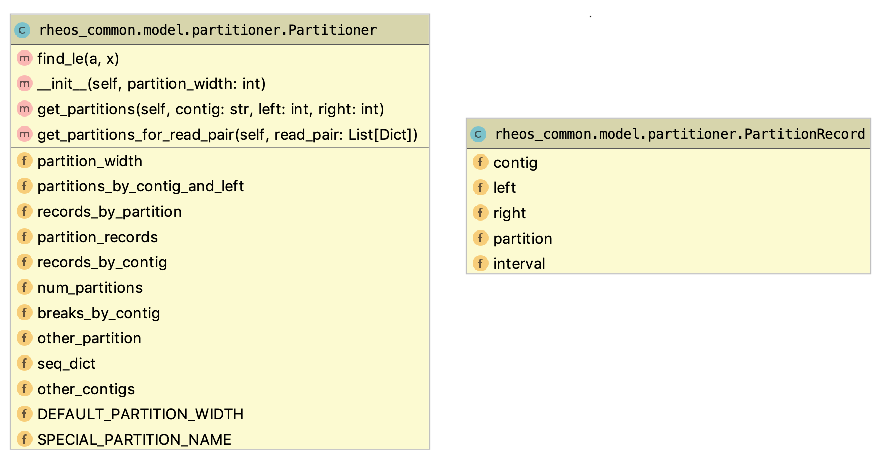
\includegraphics[scale=0.55]{rheos_partitioner_class}
    \centering
    \caption {Rheos Partitioner class diagram.}
    \label{fig:rheos_partitioner_class}
\end{figure}

Algorithm \ref{ag:partitioner} is implemented in Rheos via the \mintinline{python}{Partitioner} and \mintinline{python}{PartitionRecord} classes of the \mintinline{python}{rheos-common} package. Namely, members of $P$ are implemented as instances of \mintinline{python}{PartitionRecord}, function {\sc initializePartitioner}$(g\_main, g\_other, partition\_width)$ is implemented in \mintinline{python}{Partitioner.__init__()}, function {\sc getPartitionsForInterval}$(contig, left, right)$ is implemented in \mintinline{python}{Partitioner.get_partitions()} method, and function {\sc getPartitionsForReadPair}$(read\_pair)$ is implemented in \mintinline{python}{Partitioner.get_partitions_for_read_pair()}.

In our tests we have been using a partition width of $2\times10^7$ bases, resulting in 148 partitions for read data. The Partitioner is used in the Read Mapping Service to determine which partition to write data to, as well as in the Locus Processor Service to determine which partition is assigned to which instance of the service.

\subsection{Deployment}

Deployment of large-scale distributed systems can be complex as each component can have its own requirements related to computational resources, environment, or the ability to scale. This heterogeneity of requirements demands a flexible deployment approach that can cater to the individual needs of the various components of the system. Additionally, there is a wide variety of computational infrastructures into which a user may wish to deploy the system, again with a distinct set of capabilities and limitations. With Butler (see Chapters \ref{ch:butler_architecture}, \ref{ch:butler_implementation}) we solve this problem by utilizing a separate framework (Terraform) for abstracting the specifics of cloud provider's provisioning API, another separate framework (Saltstack) for providing a flexible configuration management facility that can configure software on a variety of platforms, and a separate suite of frameworks (InfluxDB, Grafana, Telegraf, Kapacitor) for operational management of the deployed components. We take a somewhat different approach with Rheos, one that based on the containerized nature of Rheos services, and one that relies on a single common execution environment being deployed on top of any cloud provider, or other types of computational infrastructure. The environment that we use is Google Kubernetes\autocite{bernstein2014containers}. 

\begin{figure}[H]
    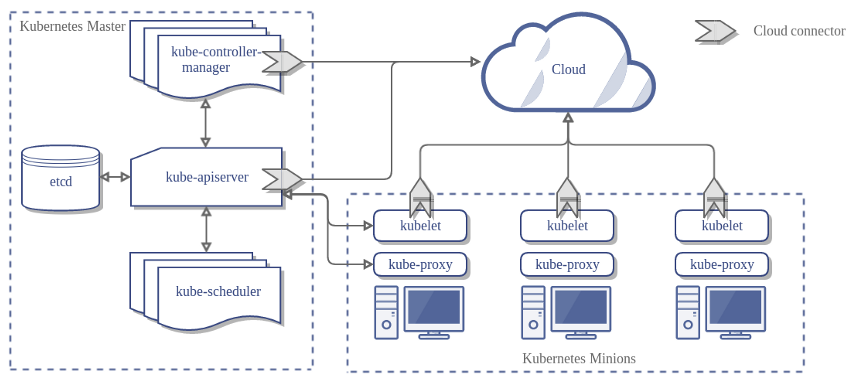
\includegraphics[scale=0.48]{kubernetes_architecture}
    \centering
    \caption {Kubernetes high level architecture (https://kubernetes.io/docs/concepts/architecture).}
    \label{fig:kubernetes_architecture}
\end{figure}

Kubernetes is a cluster resource management and container execution framework developed by Google. It can deploy on virtually any cloud as well as bare metal hardware (which makes it more flexible than the approach adopted in Butler). A Kubernetes cluster is a collection generic compute hosts (Nodes) each running the \mintinline{shell}{Docker} and \mintinline{shell}{kubelet} daemons. These nodes go into a generic pool of computational resources, although nodes with specialized capabilities, such as high RAM, or advanced GPUs can be held in separate pools. A master node is responsible for keeping track of the configuration and computational capabilities of the cluster by virtue of an etcd registry that it keeps. This node runs a special management daemon called \mintinline{shell}{kubeadm} and schedules the deployment and execution of workloads on the cluster, all of which are encapsulated in Docker containers. See Figure \ref{fig:kubernetes_architecture} for the general high level architecture of Kubernetes. This architecture is scalable to over 2500 compute nodes per cluster\autocite{scalingkubernetes}.

In order to facilitate inter-container communication Kubernetes provides an overlay network that is responsible for managing address translation, network security, and local DNS by running a proxy agent \mintinline{shell}{kube-proxy} on each node. This allows various components of the system to refer to each other by name rather than IP address, and enables role-based access to various network resources.

\begin{figure}[h!]
    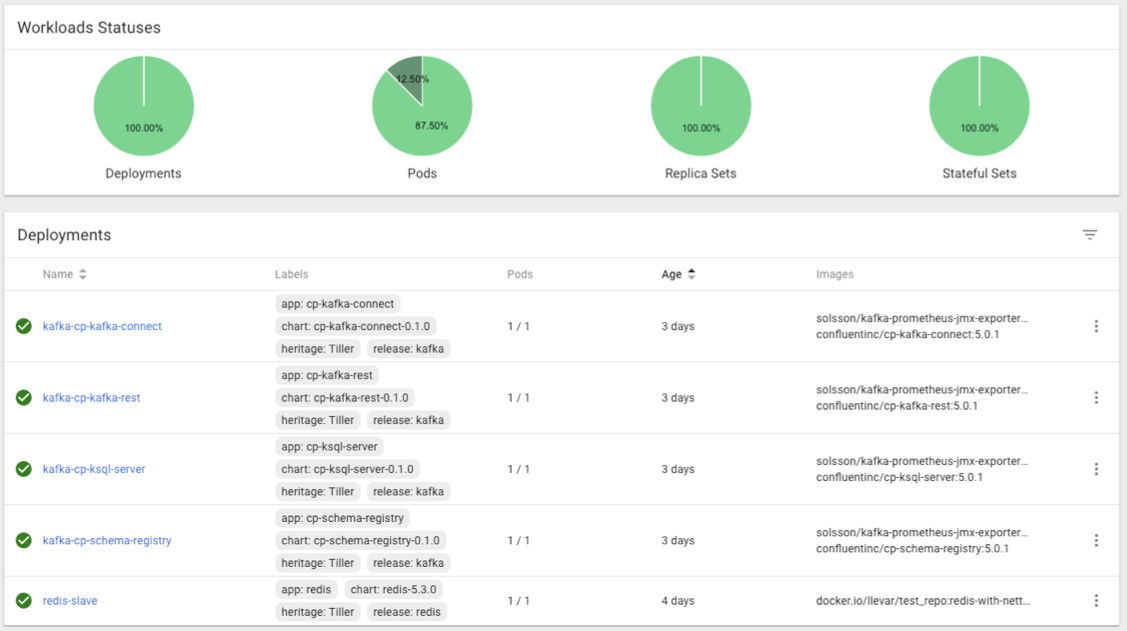
\includegraphics[scale=0.375]{kubernetes_dashboard}
    \centering
    \caption {Kubernetes dashboard.}
    \label{fig:kubernetes_dashboard}
\end{figure}

Kubernetes was built for deploying and operating services and provides a large number of high-level abstractions to facilitate the full service lifecycle. Kubernetes objects are managed through declarative documents in YAML format that describe the desired state of the system. The user interacts with the cluster by virtue of a CLI (\mintinline{shell}{kubectl}) running on the master node, or via a GUI dashboard (see Figure \ref{fig:kubernetes_dashboard}).

\begin{figure}[h!]
    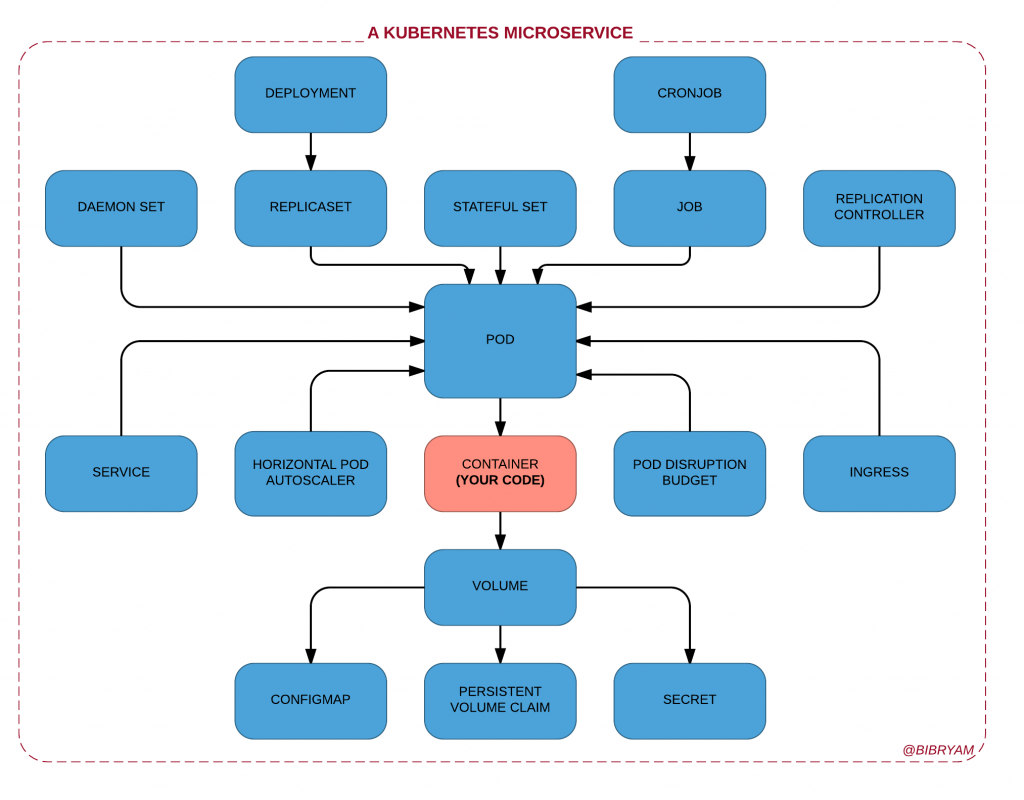
\includegraphics[scale=0.55]{kubernetes_service_components}
    \centering
    \caption {Kubernetes microservice components (from \autocite{kubernetes_microservice_components}, by Bilgin Ibryam)}
    \label{fig:kubernetes_service_components}
\end{figure}

At the lowest level of abstraction in Kubernetes hierarchy is a Pod. The Pod is a wrapper around a Docker container and describes some useful metadata for categorizing as well as describing the resource requirements of the underlying container that are used for scheduling the container onto nodes. These resources include CPU and memory requirements, as well as requests for various types of storage (called a PersistentVolumeClaim). A Pod is scheduled for execution only when the cluster manager can find a suitable node that can meet all of the pod's resource requirements. If the Pod exceeds its stated resource requirements during its lifetime it will be terminated by the scheduler.

Since the goal of kuberenetes is to enable computation at scale, Pods are rarely run as single instances. Depending on the intended usage of the underlying container Pods can be organized in groups such as a DaemonSet, ReplicaSet, StatefulSet, Job, etc. These abstractions describe the runtime behaviour of groups of Pods and provide lifecycle management support for each. For instance, a ReplicaSet provides a group stateless interchangeable Pods where each Pod can identically service a request from a client, and Pods can be scaled horizontally. The configuration for a ReplicaSet may specify the number of such Pods that should be running at a given time and the scheduler will create and delete Pods as necessary to make sure that the requisite number of Pods is running. Other groups of Pods that do not scale horizontally, and require access to non-ephemeral secondary storage (such as those running a database) may use the StatefulSet to provide such services. A DaemonSet makes sure that every node in a cluster is running an instance of a particular Pod. A Service is a higher level abstraction that provides a logical grouping of pods and provides a number of capabilities such as DNS, load balancing, and security.  

In Rheos we make use of Kubernetes for two purposes - one is to deploy and configure the various products that Rheos services rely on for their operation. These include:

\begin{description}
    \item [Kafka] - The queueing framework that all Rheos services use for communicating is deployed on Kubernetes as a set of fault tolerant Docker containers.
    \item [Redis] - Is a scalable in-memory key-value data store that Rheos services use to store intermediate results.
    \item [PostgreSQL] - Is an SQL database used for persisting variants to disk.
    \item [Prometheus] - Is a monitoring and alerting framework used to maintain operational control of the running system.
    \item [Grafana] - Is a metrics dashboarding software used for visualization of health metrics.
    \item [Elasticsearch] - Is an indexing product used for harvesting and storing application logs. 
    \item [Jenkings] - Is an automated build and deployment tool used for creating software builds.
    \item [Kubernetes Dashboard] - Is a UI used for managing Kubernetes clusters.
\end{description}

For each product we maintain a set of configuration files used for Kubernetes deployments and configuration of these tools (see Figure \ref{fig:rheos_kubernetes_configs}).

\begin{figure}[h!]
    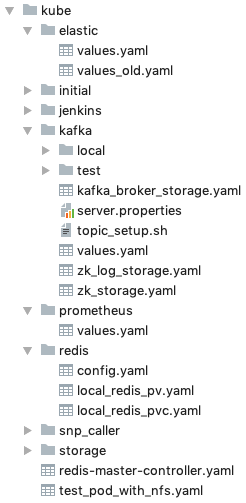
\includegraphics[scale=0.55]{rheos_kubernetes_configs}
    \centering
    \caption {Rheos Kubernetes configurations file layout.}
    \label{fig:rheos_kubernetes_configs}
\end{figure}

Additionally we use Kubernetes to configure and deploy the services of Rheos themselves, organized as fleets of Docker containers. This allows us to enjoy the flexibility of being able to deploy on virtually any hardware, the envirnment isolation provided by Docker, and the resource management and elastic scalability afforded by Kubernetes, which are all key concerns when operating a large-scale service-oriented system.

\subsection{Services of Rheos}

We build on top of the concepts of a general Rheos Service, Kafka topics, the Kubernetes framework and other products described earlier in this section to provide a cohesive implementation of a set of services that implement two major end-to-end use cases encountered in genomic analysis - germline SNP calling, and germline SV (deletion) calling. As Rheos matures these services will be extended to provide enhanced functionality and increased scalability required for production applications of the framework. 

\subsubsection{Read Mapping Service}

The Read Mapping Service is the entrypoint of the initial Rheos implementation. Although future versions of Rheos will likely have a different entrypoint, namely a Read Streaming Service that will accept data from an external endpoint, such as a data repository or directly from the sequencer, we proceed directly to read mapping in this initial implementation as a matter of simplification. 

This service aims to implement two read mapping operations specified in Section \ref{sec:main_body_alignment} - $mapToReference()$ and $mapPairToReference()$. It reads a user-specified FASTQ file (the sample), as well as a genome reference file from disk and emits four data streams $mappedReads$, $mappedReadPairs$, $unmappedReads$, and $unmappedReadPairs$. These operations allow the service to deal with both paired and unpaired short reads produced by Illumina sequencers. The partitioning strategy of Section \label{sec:main_body_partitioning} implemented in the \mintinline{python}{rheos-common} package is used to determine which partition of their respective topics reads end up in. Instead of implementing our own read mapper from scratch we are making use of a python module called \mintinline{python}{mappy}, which is an interface to the popular read alignment tool minimap2\autocite{Li2018}, by Heng Li, which is based on the hashmap approach to alignment discussed in Section \ref{sec:bg_alignment}. The reason we chose to provide a wrapper rather than a full implementation is that minimap2 already has an API that supports a read-by-read alignment that can be adopted for a streaming use case. Additionally, minimap2 is known to be accurate, fast, and supports mapping of long reads, and other use cases, making it an attractive framework to work within for read alignment.

Although the Read Mapping Service can map and stream individual reads, this approach proves quite impractical. In our tests of performance, we observed that for a single read the cost of serializing the mapped read data to send it over the wire was nearly 40\% of the overall processing time. To reduce the proportion of computational resources used for serialization/deserialization we implemented a read batching strategy based on the reservoir concept, that groups similar reads together and sends them over the wire as a group. A \mintinline{python}{PartitionedReservoirSet} that implements this functionality is shown in Figure \ref{fig:partitioned_reservoir_set}.

\begin{figure}[h!]
    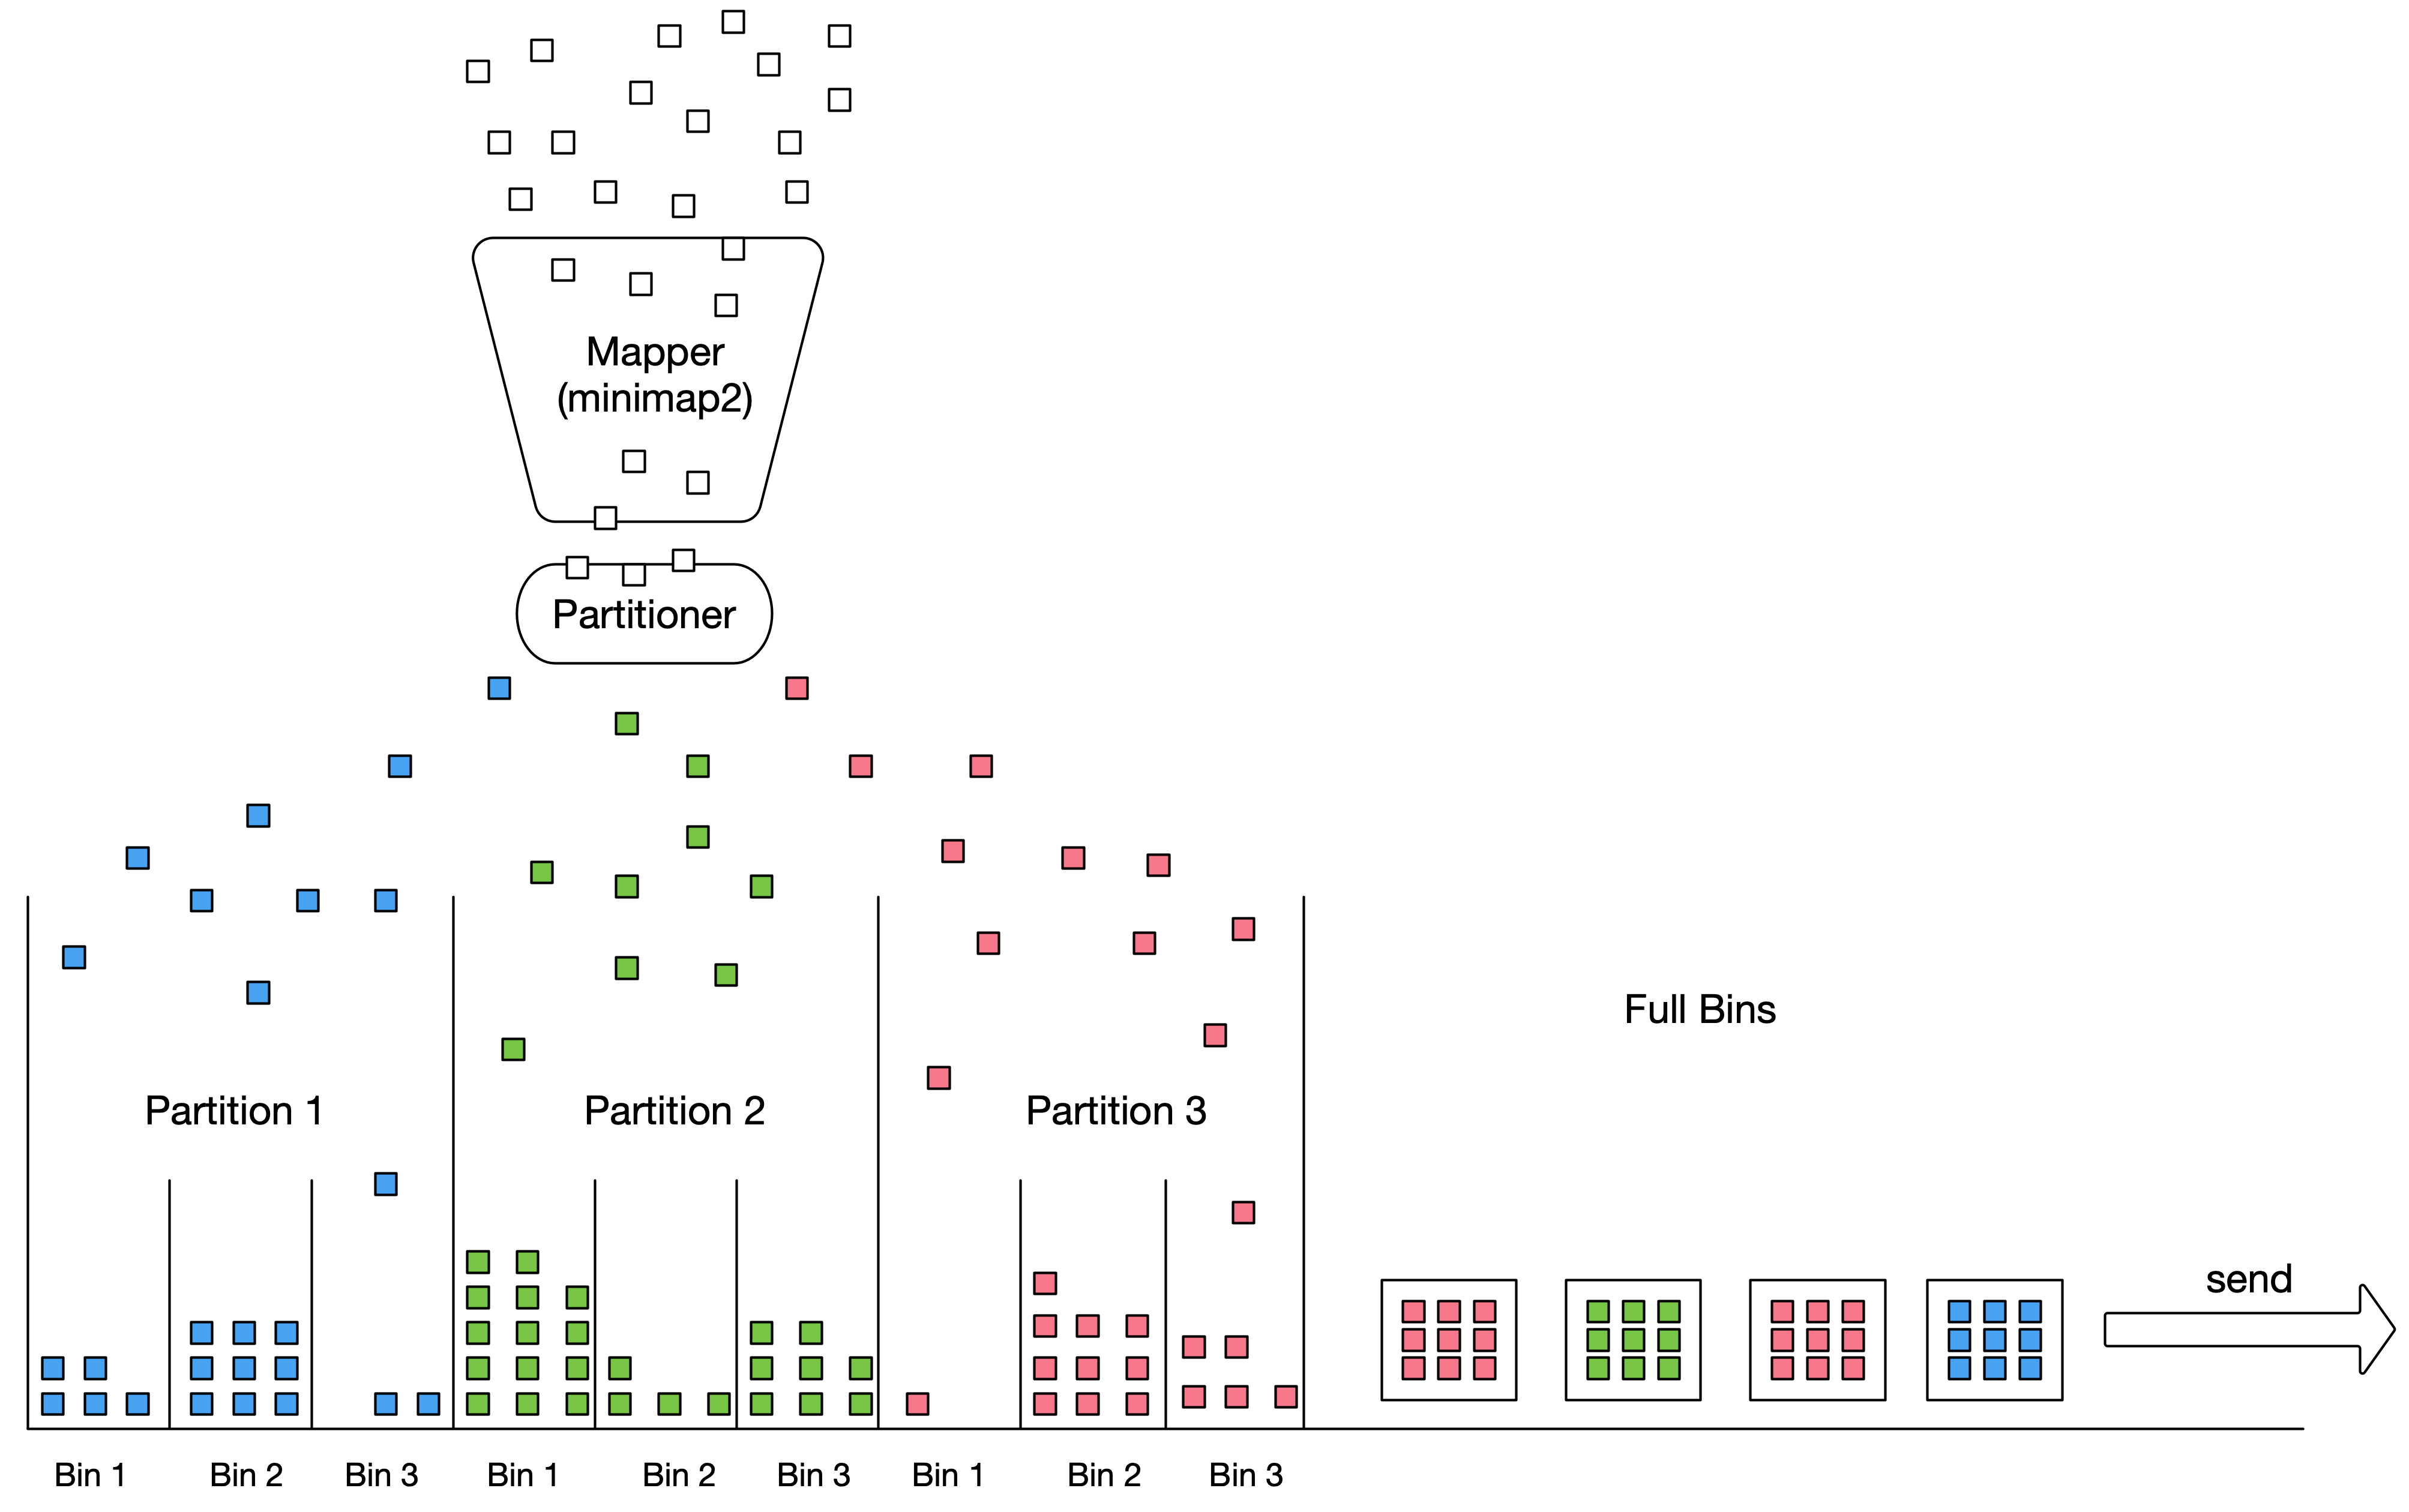
\includegraphics[scale=0.43]{partitioned_reservoir_set}
    \centering
    \caption {A \mintinline{python}{PartitionedReservoirSet} is used to group together similar reads before streaming them as a mini batch.}
    \label{fig:partitioned_reservoir_set}
\end{figure}

Reads are read one-by-one from a FASTQ file. Each read is attempted to be paired. If no pair exists for the read it is put into an accumulator (a type of hashmap). If a read completes a read pair, it is popped from the accumulator and the read pair is sent through to alignment by minimap2. Once the read pair is aligned it is put through the Partitioner to assign a set of PartitionRecords to it. Each PartitionRecord is further subdivided by genomic interval into a set of bins that act as reservoirs. The size of the bins is controlled by user supplied parameters where $num\_bins$ specifies how many bins are created per partition, and $bin\_size$ specifies capacity in read pairs. Each \mintinline{python}{Reservoir} accumulates read pairs that map within its genomic region, until reservoir capacity is reached. At that point all of the read pairs from that reservoir are serialized and emitted from the service as a single message. The reservoir is then emptied and is ready to accept new elements. When a whole sample is finished alignment all of the non-empty bins are serialized and emitted by the service as individual messages. Figure \ref{fig:rheos_read_mapping_service_classes} shows the classes and methods of the Read Mapping Service and the \mintinline{python}{PartitionedReservoirSet}.

\begin{figure}[h!]
    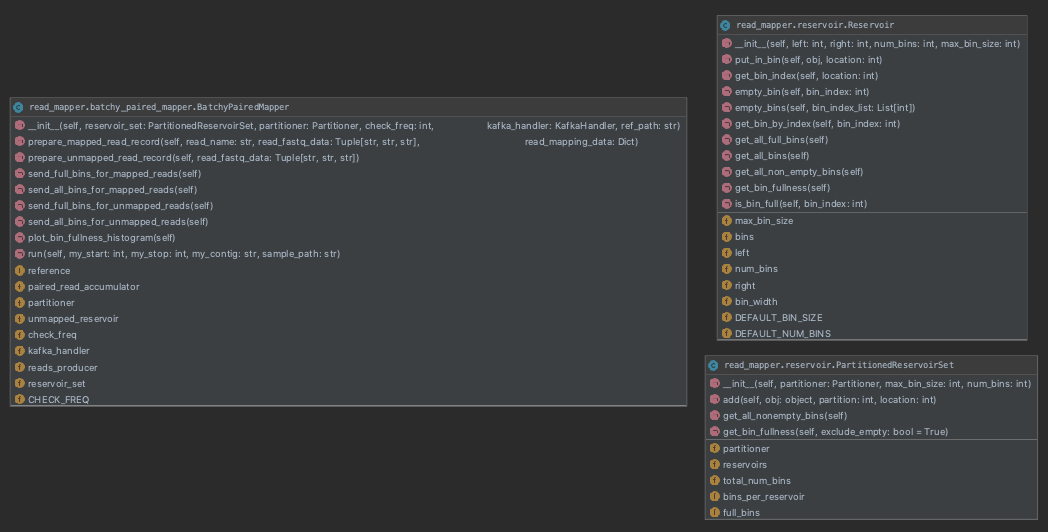
\includegraphics[scale=0.405]{rheos_read_mapping_service_classes}
    \centering
    \caption {Classes of the \mintinline{python}{ReadMappingService}.}
    \label{fig:rheos_read_mapping_service_classes}
\end{figure}

The disadvantages of the mini-batching approach are the decreased initial throughput (no data is emitted by the service before at least one of the reservoirs fills up), and increased memory footprint of the Read Mapping Service. The reservoir approach, however, reduces the proportion of the overall processing time due to serialization by over 90\%. Additionally, there are benefits to processing the read data in small batches of closely-mapped reads by downstream services, because all of the loci that need to be updated by the reads can be fetched into memory and efficiently processed, and the since the reads map closely together, fewer total loci are updated by such a batch than by a random collection of reads. In general, since the usage of the \mintinline{python}{PartitionedReservoirSet} can be controlled by the user via service parameters, there is a good degree of flexibility when it comes to trading off these performance considerations.

\subsubsection{Locus Processor Service}

The Locus Processor Service is a Rheos service that listens to the stream of mapped read pairs produced by the Read Streaming Service and updates a set of genomic loci that the reads overlap with the variant evidence contained in the reads. It then emits a stream of updated loci that can be further processed by downstream services for variant calling. Figure \ref{fig:rheos_locus_processor_service} shows a schematic view of the Locus Processor Service.

\begin{figure}[h!]
    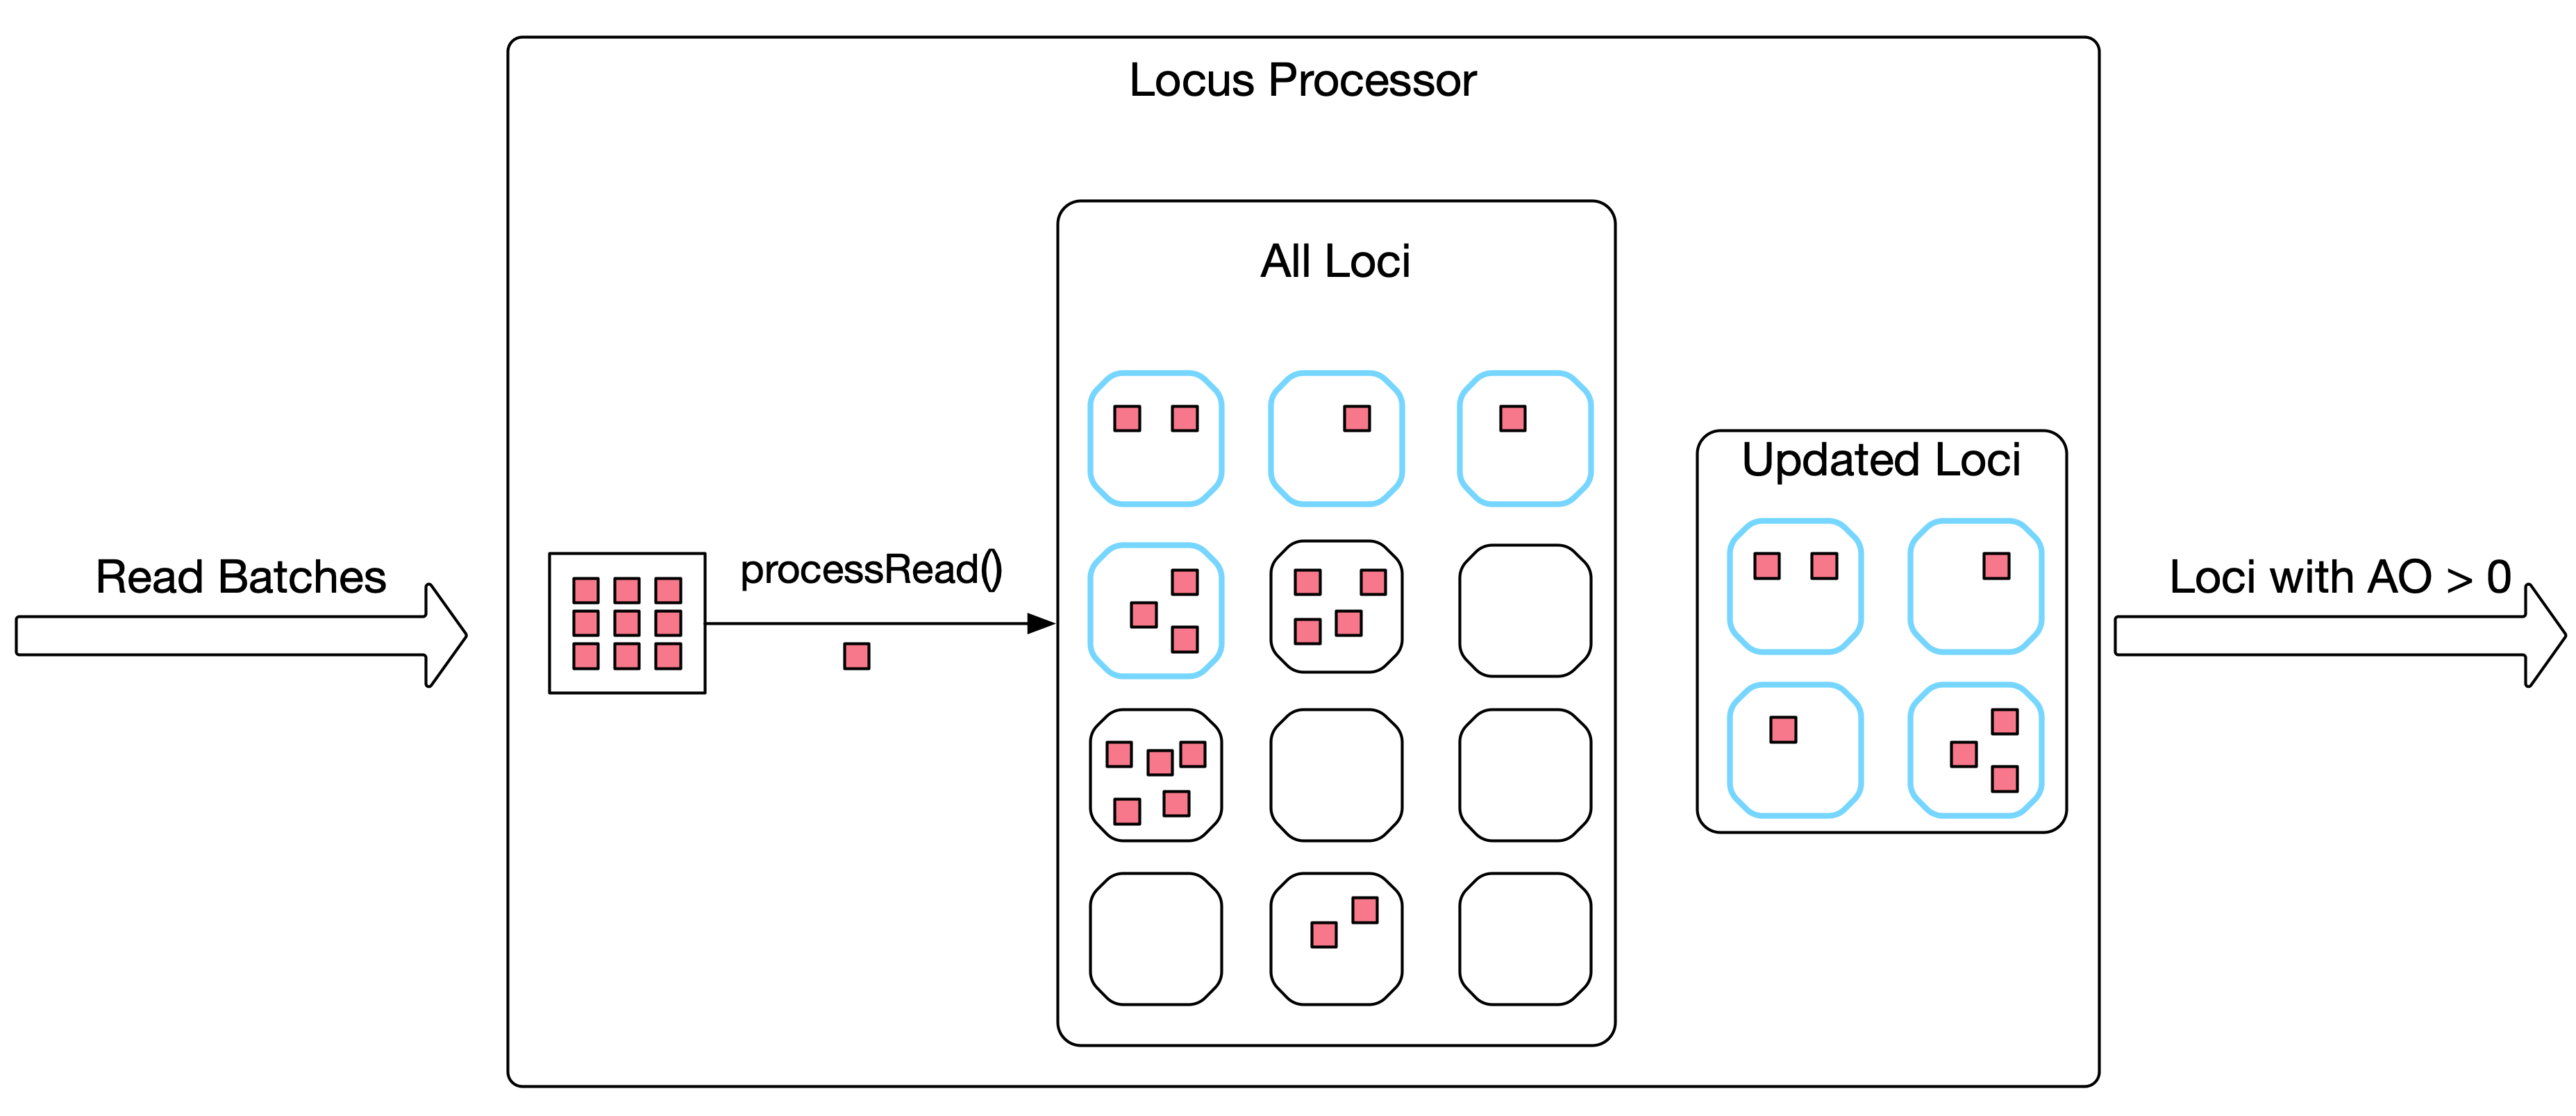
\includegraphics[scale=0.405]{rheos_locus_processor_service}
    \centering
    \caption {The Locus Processor Service uses read data to update a set of loci.}
    \label{fig:rheos_locus_processor_service}
\end{figure}

The Locus Processor Service is of Local State Aggregator type and implements the iterative Bayesian inference framework described in Section \ref{sec:main_body_germline_snp_calling}, namely it implements the stream operation $updateLociFromRead()$, Equations \ref{eq:rheos_genotype_likelihood}, and Algorithms \ref{ag:process_read_pair}, and \ref{ag:handle_match}. The service uses the same Paritioner to decide where to get data from as is used by the Read Mapping Service.

A single message received by the Locus Processor Service represents a full bin of mapped read pairs from a single partition of the $mapped\_read\_pairs$ kafka topic. \mintinline{python}{BatchyPairedLocusProcessor.process_messages()} is the main processing loop of the service (see Figure \ref{fig:locus_processor_classes}). An in-memory collection of \mintinline{python}{Locus} objects for the assigned parition, organized in a hashmap by genomic coordinate is the main holder of state for the service. For each received message, the \mintinline{python}{BatchyPairedLocusProcessor.process_reads()} method is responsible for processing all of the contained reads. It acts as the implementation of Algorithm \ref{ag:process_read_pair}.

Namely, for each read, the algorithm simultaneously walks the genome reference and the read CIGAR string looking for matches. Different CIGAR elements consume the reference, the read, or both. For instance, a deletion consumes the reference sequence, but not the read. It's the opposite case for an insertion, and a sequence match consumes both. Deletion and insertion CIGAR elements will in the future be used for indel variant calling, but at the moment they are simply passed over. When a match CIGAR element is found, the \mintinline{python}{BatchyPairedLocusProcessor.handle_match()} method is called.

\begin{figure}[h!]
    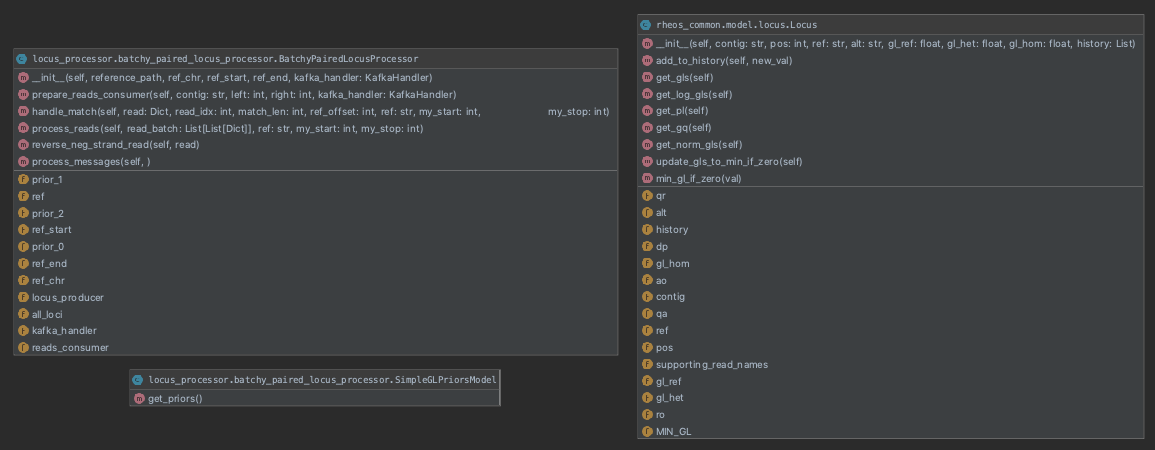
\includegraphics[scale=0.36]{locus_processor_classes}
    \centering
    \caption {The Locus Processor Service classes and methods.}
    \label{fig:locus_processor_classes}
\end{figure}

This method implements Algorithm \ref{ag:handle_match}. For each match the set of \mintinline{python}{Locus} objects overlapping the match are retrieved. The model of each \mintinline{python}{Locus} is updated using Equation \ref{eq:rheos_genotype_likelihood}, depending on whether that position in the read matches the reference. Reads that map to the negative strand are reverse complemented using \mintinline{python}{BatchyPairedLocusProcessor.reverese_neg_strand_read()} and matched from the end.

For each input message received, all \mintinline{python}{Locus} models that have been updated by reads in this message, and that potentially have variants (determined by \mintinline{python}{Locus.AO} > 0, where AO is the count of alternative allele observations for that locus) are bundled together and emitted as a single message of updated loci from the Locus Processor Service.

\subsubsection{Locus Saver Service}

The Locus Saver Service is a fairly simple service that acts as an aggregating and persistence mechanism for \mintinline{python}{Locus} objects. Rheos uses an open source in-memory distributed key-value store called Redis\autocite{carlson2013redis}. Using this product allows Rheos to keep a large number of \mintinline{python}{Locus} objects in memmory for fast retrieval, while offering options for distributed access and optional disk persistence.

\begin{figure}[h!]
    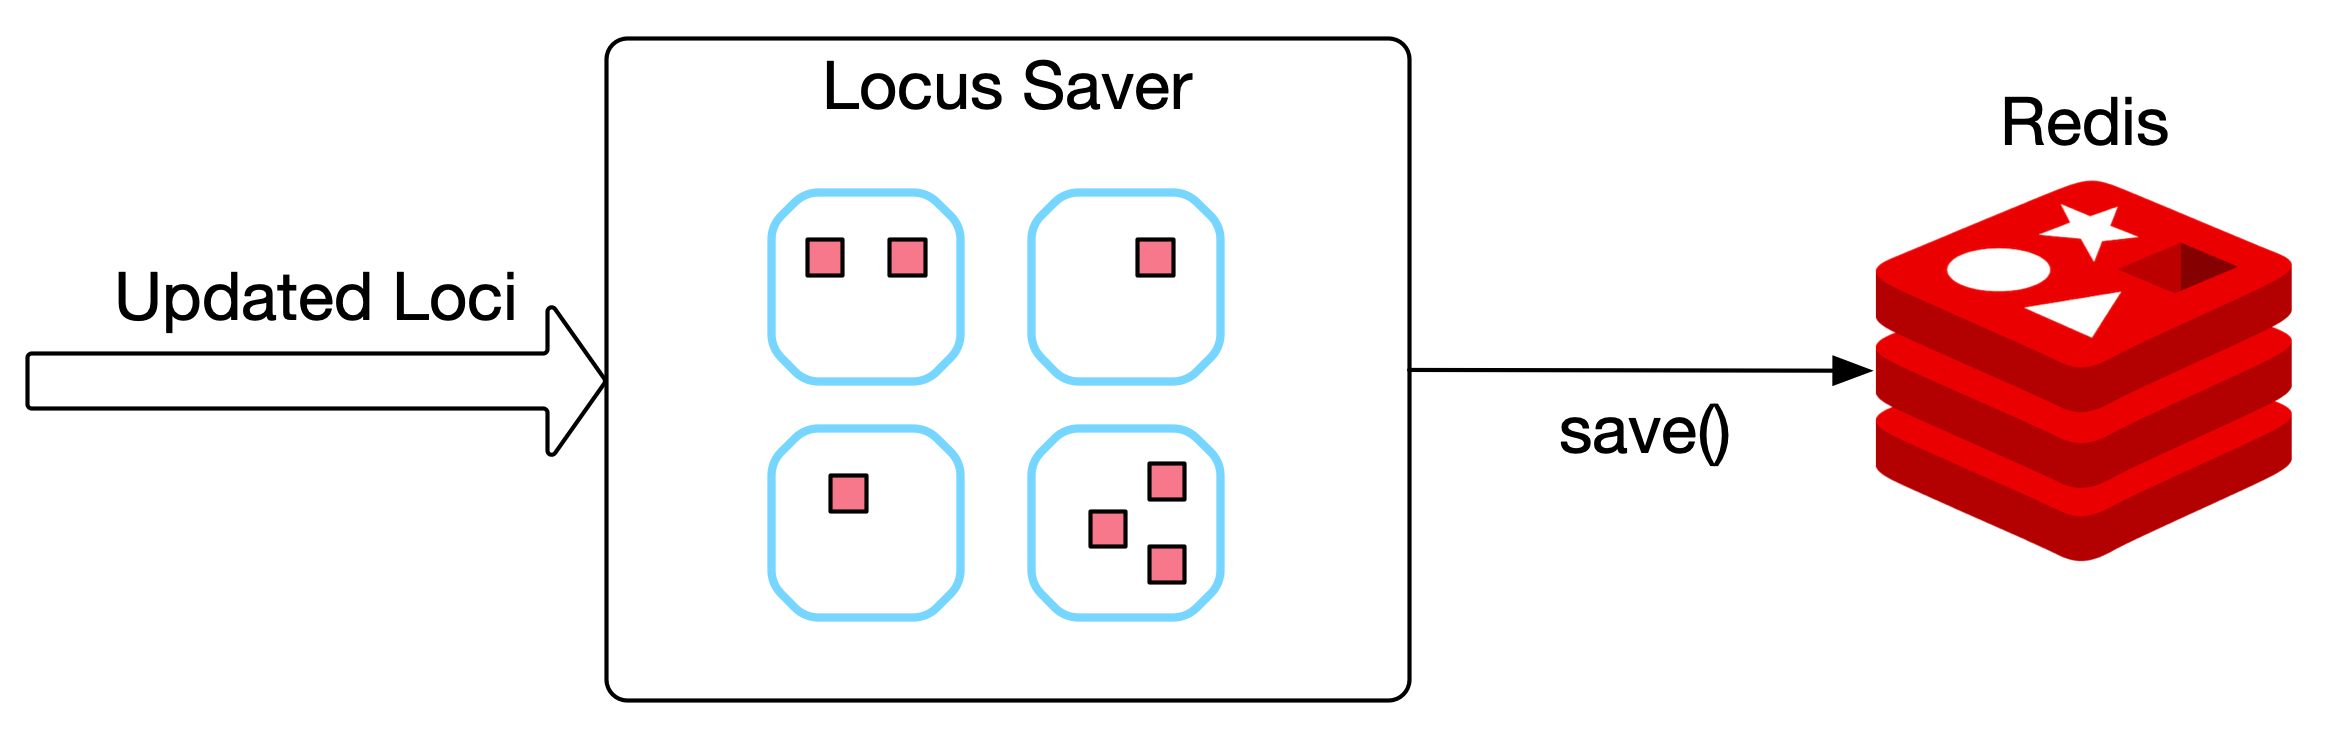
\includegraphics[scale=0.55]{rheos_locus_saver_service}
    \centering
    \caption {The Locus Saver Service data processing schematic.}
    \label{fig:rheos_locus_saver_service}
\end{figure}

The Locus Saver Service recieves messages from the $snp\_loci\_batchy$ kafka topic, where each message contains a batch of updated \mintinline{python}{Locus} objects. The service writes all of the updated loci to Redis potentially overwriting any existing values.

\subsubsection{Variant Calling Service}

The Variant Calling Service is not a stream-based service, instead it provides a querying interface into Rheos via its $callVariants(region, calling\_threshold)$ operation, where the user provides a region of interest and variant quality threshold and the service creates a VCF file of all called variants in the region that meet the variant quality criteria. 

\begin{figure}[h!]
    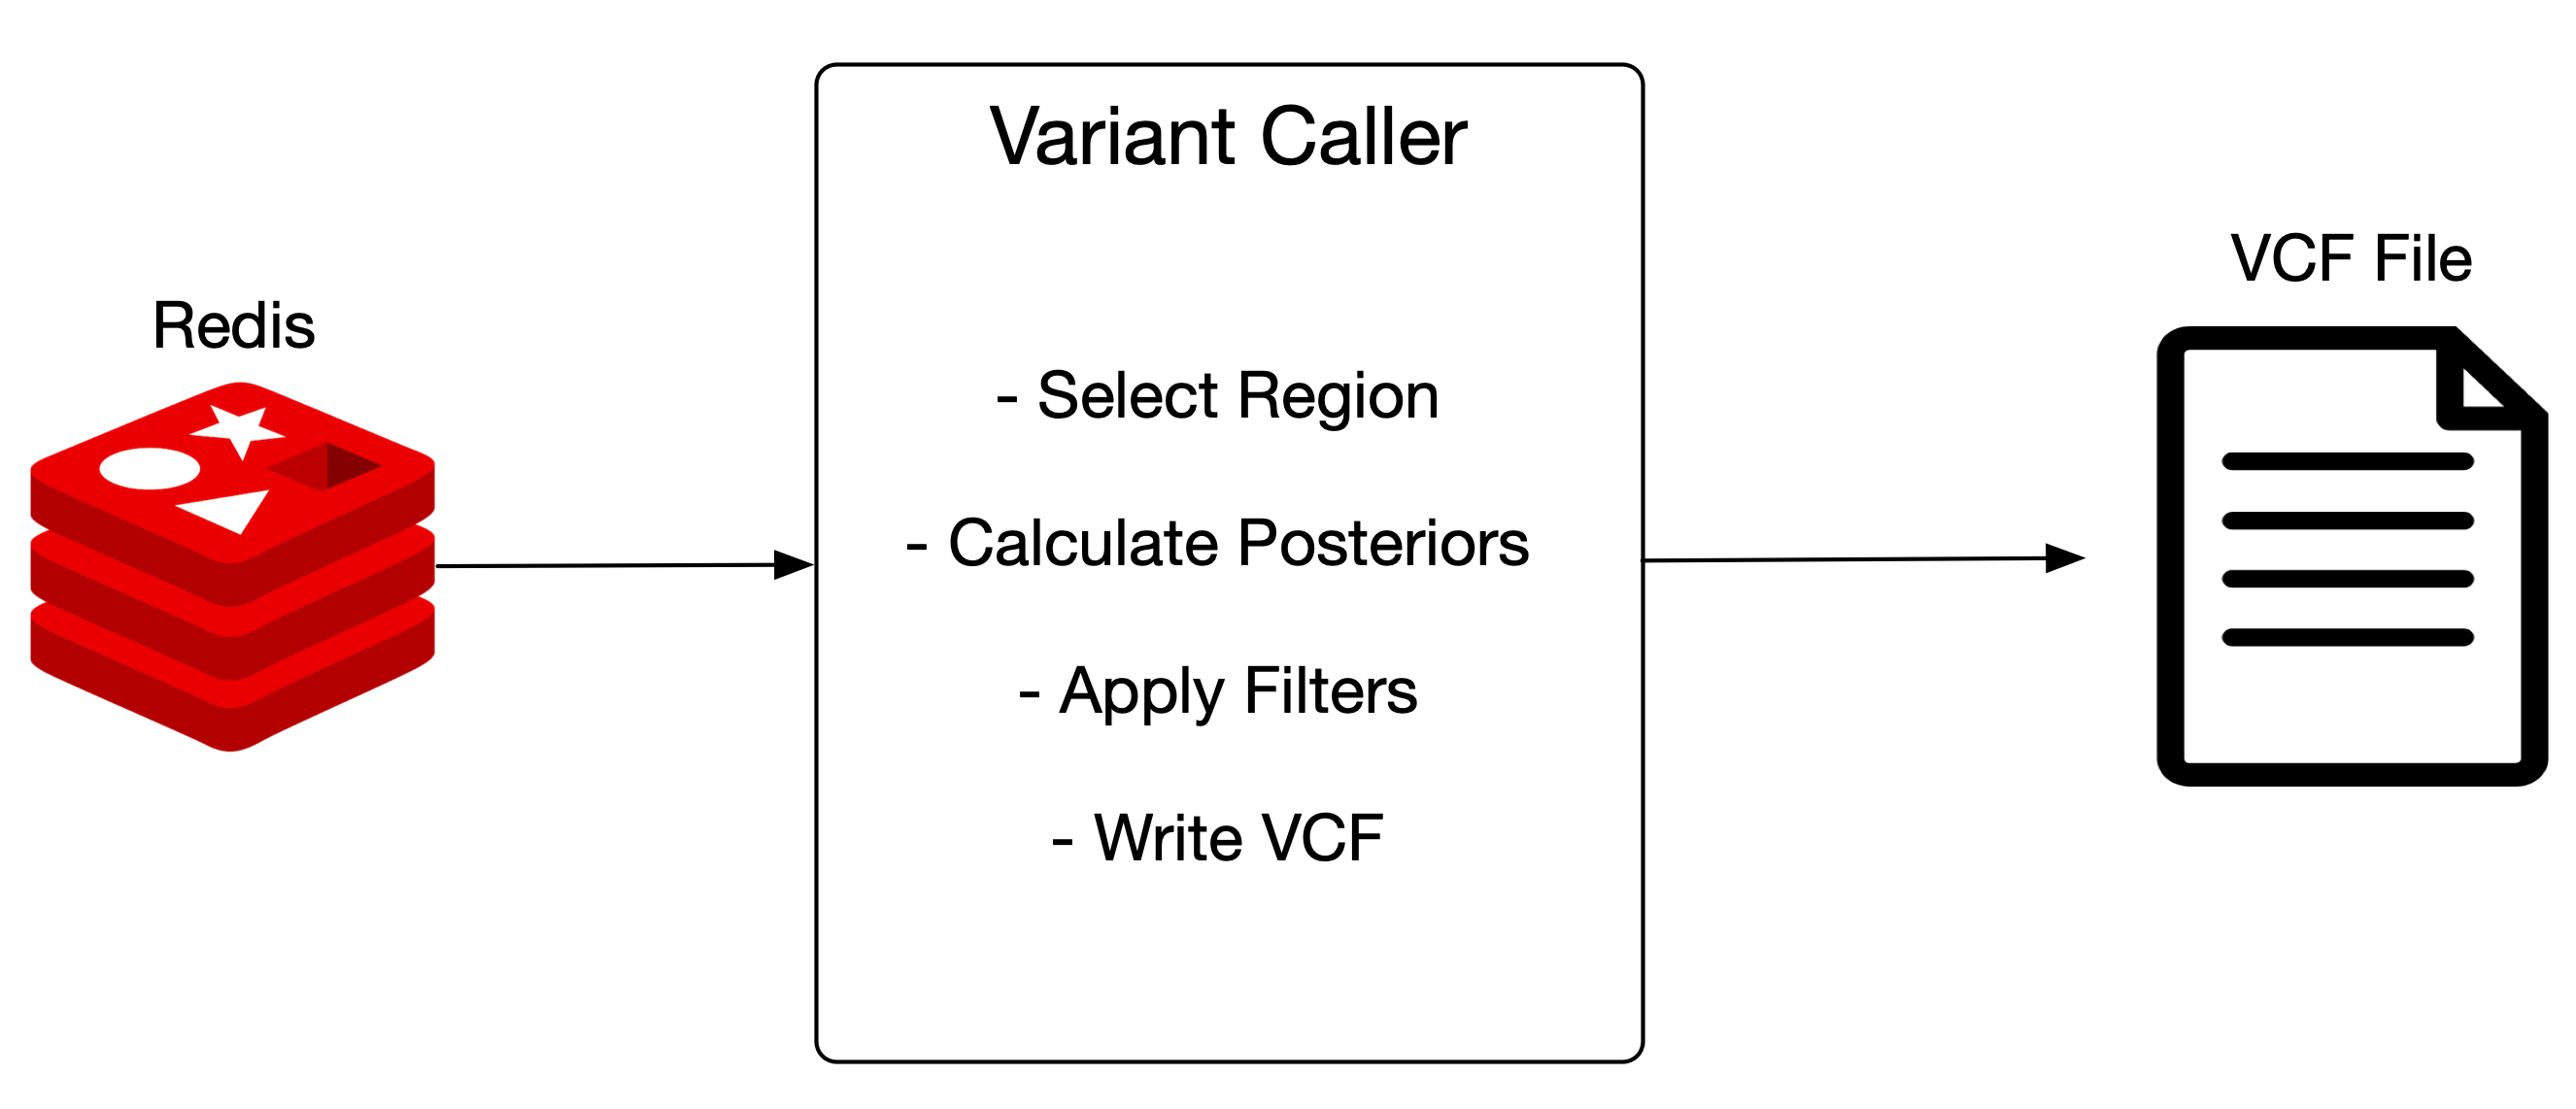
\includegraphics[scale=0.55]{rheos_variant_calling_service}
    \centering
    \caption {The Variant Calling Service data processing schematic.}
    \label{fig:rheos_variant_calling_service}
\end{figure}

This service communicates with the Redis locus store (see Figure \ref{fig:rheos_variant_calling_service}) and retrieves all of the loci that match the query region. For each locus it calculates the posterior genotype probabilities via Equation \ref{eq:rheos_genotype_posterior}. Variants the exceed the user provided quality threshold will be written to the output VCF file. It is possible to apply other variant filtering criteria at this stage to improve calling stringency. As the service requires access to secondary storage it is deployed as a StatefulSet under Kubernetes.

\subsubsection{Insert Size Filtering Service}

The Insert Size Filtering Service is a streaming service of Filter type. It implements the $filterDiscordantPairs()$ operation in order to obtain a stream of read pairs that are fit for germline deletion calling as described in Section \ref{sec:main_body_sv_calling}. The service initially only accumulates read pairs in order to estimate the insert size distribution. The default initial sample size for this purpose is 100000 read pairs, but this value is controlled by the user. Using this sample we estimate the median insert size, and subsequently the Median Absolute Deviation of the insert size which acts as our cutoff for discordantly mapped reads. Once the estimate is obtained we send the accumulated reads through the rest of the filtering process, followed by any other new read pairs that are observed in the data stream. Read pairs that pass filtering are sent to the $discordant\_read\_pairs$ kafka topic. 

\subsubsection{Insert Size Clustering Service}

The Insert Size Clustering service implements the $addReadPair()$ streaming operation and the $callDeletions()$ querying operation. $addReadPair()$ observes the $discordant\_read\_pairs$ data stream and adds any messages that are received into the internal data structures used for deletion calling. 

\begin{figure}[h!]
    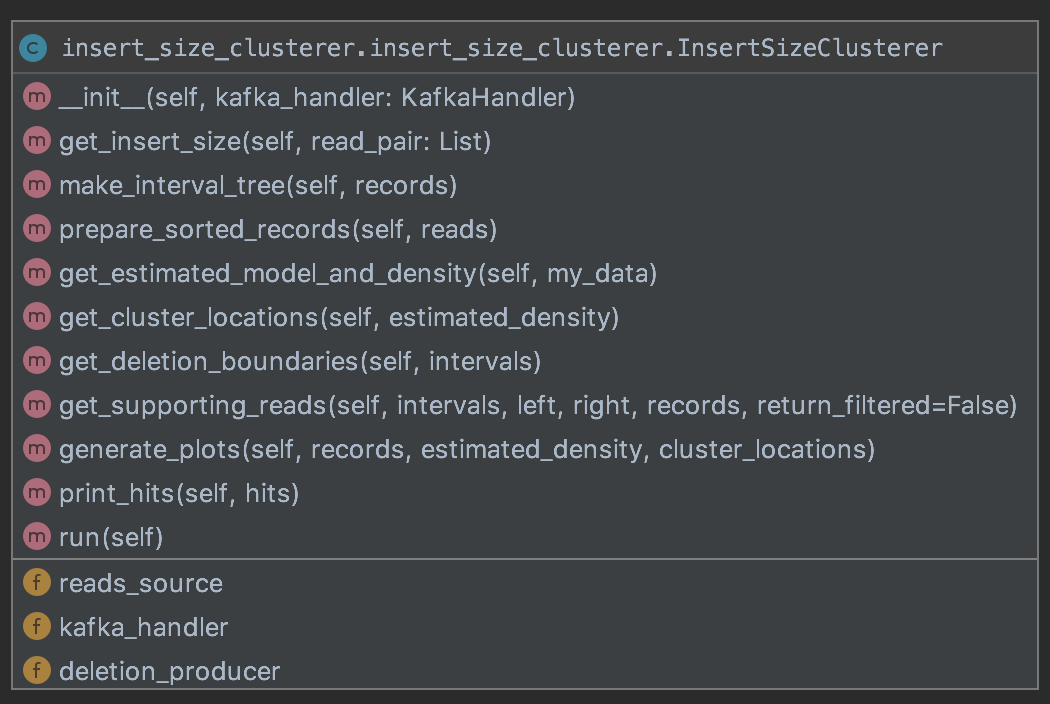
\includegraphics[scale=0.55]{insert_size_clusterer_class}
    \centering
    \caption {The Insert Size Clusterer class methods.}
    \label{fig:insert_size_clusterer_class}
\end{figure}

The reads are stored as both a List for general handling and clustering, as well as an Interval Tree (see Figure \ref{fig:interval_tree}) - a type of balanced binary search tree useful for finding interval overlaps. We use an open source implementation of the Interval Tree from https://github.com/chaimleib/intervaltree.

When $callDeletions()$ is executed the accumulated reads are prepared for processing by finding their center and insert size. The read centers are then clustered using the \mintinline{python}{KernelDensity} object from the \mintinline{python}{sklearn.neighbors} Python package (see Figure \ref{fig:kde}). Peaks of the estimated distribution are found using the \mintinline{python}{argrelextrema()} function from the \mintinline{python}{scipy.signal} package. Given the location of a cluster center we find the set of read pairs that overlap the center via the Interval Tree. Given a pre-constructer Interval Tree $t$ and a cluster center coordinate $center$ we obtain the necessary set of intervals by simply calling $overlaps = t[rec.center]$.

For each set of overlap intervals the deletion size is set to be the maximum common overlap between the inner sizes of all such intervals (see Figure \ref{fig:deletion_read_cluster}). All overlapping read pairs whose $insert\_size > deletion\_size + insert\_size\_threshold$ are removed from the list of reads that support the deletion, and if the number of remaining reads is $> min\_support\_threshold$ the deletion is called as real.

\section{Experimental Validation}

We focused on two primary use cases in validating the initial implementaion of the Rheos framework. The first is the ability of the framework to accurately perform germline SNP calling. The second is the ability of the framework to accurately perform germline deletion calling. Deployment of the framework onto cloud computing infrastructure was also tested. Detailed performance testing was not performed because of the limited scope of the project.

\subsection{Deployment}

The Rheos framework has been deployed onto the academic cloud computing infrastructure provided by EMBL/EBI Embassy Cloud, an OpenStack environment with 164 CPUs, 744 GB RAM, and 15 TB of block volume storage. Resources were split into 12 virtual machines with the following variety of characteristics:

\begin{table}[!ht]
    \centering
    \caption{Rheos deployment infrastructure}
    \label{tab:rheos_deployment_infrastructure}
    {\begin{tabular}{r | r | r | r}
    \toprule
    Count & CPU & RAM & Ephemeral Disk \\
    \midrule
    1 & 4 & 8GB & 60GB\\
    4 & 8 & 32GB & 100GB\\
    6 & 16 & 64GB & 100GB\\
    1 & 32 & 224GB & 100GB\\
    \bottomrule
    \end{tabular}}
\end{table}

One VM with 4 CPU and 8 GB RAM was designated as the Kubernetes master node, with other small services like the Kubernetes Dashboard and Weave Networking Dashboard deployed to it as well. Other VMs were put into the pool of worker nodes with automated deployment scheduling of Docker containers provided by Kubernetes. A Weave overlay network was set up between all of the nodes in the Kubernetes cluster, creating a private subnet for inter-VM and inter-container communication but inaccessible from the outside.

The following products were set up to support the running of Rheos:

\begin{description}
    \item [Kafka] - A Kubernetes Kafka service was deployed with a redundancy of 3, deploying 3 borkers on 3 separate nodes, to ensure availability and scalability.
    \item [Zookeeper] - A Kubernetes Zookeeper service was deployed with a redundancy of 3.
    \item [Redis] - A Kubernetes Redis server was set up with 1 master and 1 replication slave.
    \item [Prometheus] - Prometheus was set up for monitoring with 1 master, and an agent running on every node.
    \item [Grafana] - Grafana was set up as a single container for monitoring dashboarding.
    \item [Elasticsearch] - Elasticsearch was set up as a single server for collection of application logs.
    \item [Jenkins] - Jenkins was set up as a single server for automated deployment and continuous integration of new builds in the testing environment.
\end{description}

\begin{figure}[h!]
    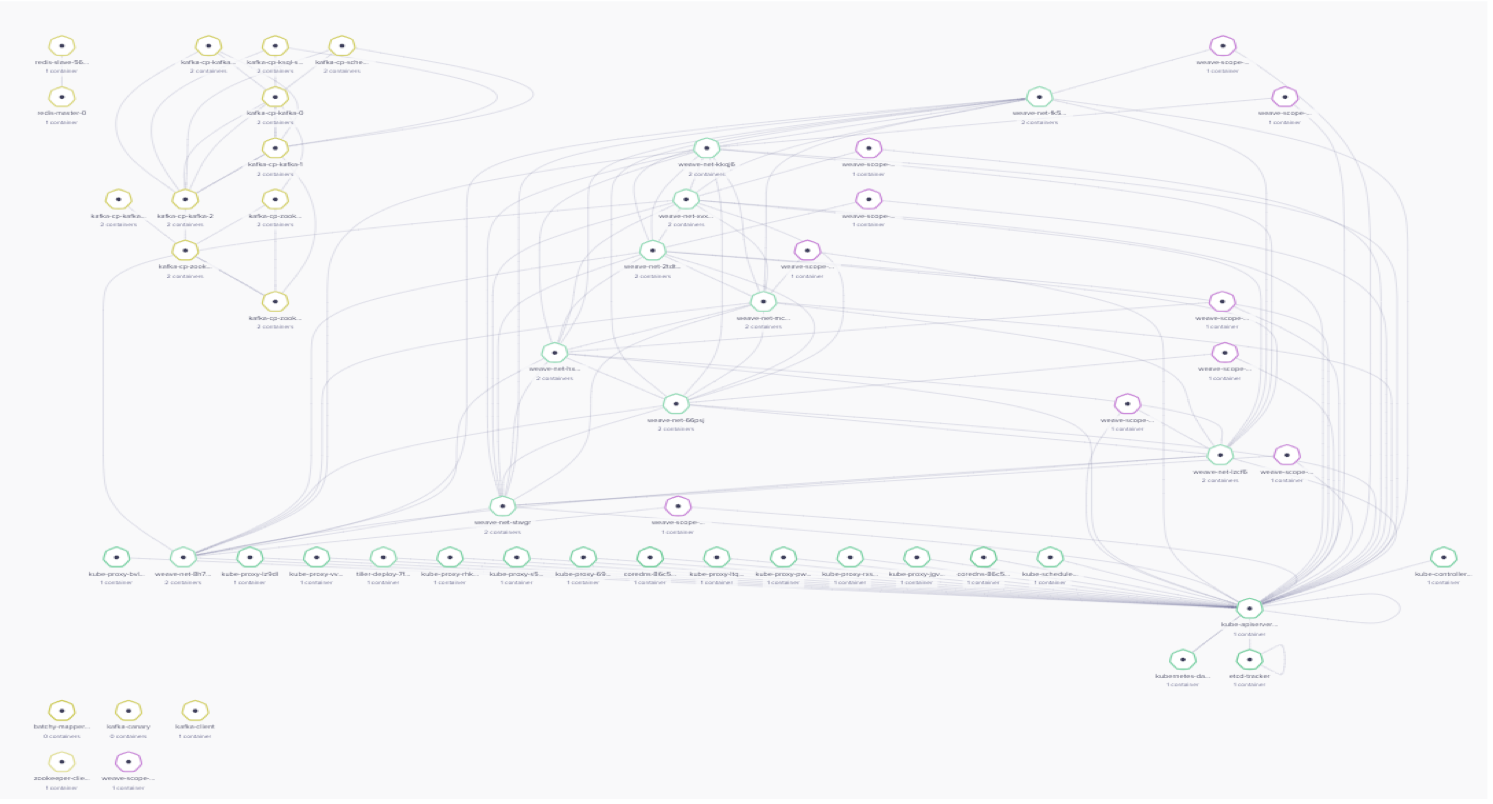
\includegraphics[scale=0.28]{rheos_deployment_containers}
    \centering
    \caption {Docker containers that are part of the test Rheos deployment.}
    \label{fig:rheos_deployment_containers}
\end{figure}

The services of Rheos were deployed into the Kubernetes environment in the following configuration:

\begin{description}
    \item [Read Mapping Service] - The service was deployed as a set of 2 Kubernetes Pods on separate nodes with access to a 500TB NFS share for reading sample data, and a local copy of the human reference genome, preprocessed for use by minimap2.
    \item [Locus Processor Service] - The service was deployed as a set of 6 Kubernetes Pods, each with a local copy of the human reference genomes in FASTA format.
    \item [Locus Saver Service] - The service was deployed as a set of 2 Kubernetes Pods on separate nodes.
    \item [Variant Caller Service] - The service was deployed as a single Kubernetes Pod, with access to a 500TB NFS share for writing the VCF file.
    \item [Insert Size Filtering Service] - The service was deployed as a single Kubernetes Pod.
    \item [Insert Size Clustering Service] - The service was deployed as a single Kubernetes Pod.
\end{description}

The following Kafka topics were set up for management of in-flight data. A replication-factor of 1 was used.

\begin{table}[!ht]
    \centering
    \caption{Rheos Kafka topics.}
    \label{tab:rheos_kafka_topics}
    {\begin{tabular}{l | r }
    \toprule
    Name & Partitions \\
    \midrule
    $mapped\_read_pairs\_batchy$ & 168\\
    $unmapped\_read_pairs\_batchy$ & 2\\
    $mapped\_read_pairs\_secondary\_batchy$ & 10\\
    $snp\_loci\_batchy$ & 2\\
    $discordant\_read\_pairs$ & 1\\
    $deletions$ & 1\\
    \bottomrule
    \end{tabular}}
\end{table}

Figure \ref{fig:rheos_deployment_containers} shows the set of Docker containers that were used in the Rheos Kubernetes deployment. In addition to the Kubernetes test environment, local testing of individual components was performed on a MacBook Pro 2018, with a 6-core 2.9 GHz Intel Core i9 processor, and 32 GB RAM. 

\subsection{Sample Selection and Preparation}

To assess the ability of Rheos to perform germline SNP and SV calling we have selected a well characterized genomic sample from the Genome in a Bottle Consortium\autocite{zook2018reproducible}, namely the NA12878 sample that was first sequenced in the context of the 1000 Genomes Project, but has subsequently been sequenced by a variety of orthogonal sequencing technologies to very high levels of coverage and is very well studied. Choosing this sample allows us to work with data that is known to be of high quality and one that has a high quality set of published genomics variants to compare Rheos calls against.

We downloaded the sample RMNISTHS\_30xdownsample.bam a 147GB file from the GIAB FTP repository at ftp://ftp-trace.ncbi.nlm.nih.gov/giab/ftp/data/NA12878/NIST\_NA12878\_HG001\_HiSeq\_300x/. This sample is a high coverage 300x sequencing run of the Illumina HiSeq 2500 instrument using a 2x148 bp paired end library. The original data has been mapped to the GRCh37d5 human reference genome using BWA-MEM, and subsequently downsampled to ~30x average coverage. 

We performed our experiments on Chromosome 20 of the sample, which is a DNA molecule that is 63025520 nucleotides long. We extracted raw unaligned reads for Chromosome 20 from the BAM file into a separate FASTQ file. The size of this FASTQ file is 4.3 GB and it contains 13424120 reads. All of the alignment information was discarded in the transformation from BAM to FASTQ.

The GRCh37 human reference genome was obtained from the 1000 Genomes Project FTP site at ftp://ftp.ncbi.nih.gov/1000genomes/ftp/technical/reference/phase2\_reference\_assembly\_sequence/. The reference is in FASTA format and is ~3GB in size. It contains the reference sequence for human chromosomes 1-22, X, Y, MT (mitochondrial) as well as a set of decoy sequences and unplaced contigs. We use the entire reference genome because reads that were mapped to Chromosome 20 by BWA-MEM may be mapped elsewhere by the minimap2 aligner. We pre-process the reference for use by minimap2 to generate a minimizer index genome.mmi using default parameters.

\subsection{Germline SNP Calling}

For germline SNP calling we put together a pipeline using Rheos services that takes a FASTQ sample file, streams the reads, maps them to a reference genome, processes the variant evidence contained in the reads, save the resulting genomic loci in a data store, and performs variant calling, outputting a result VCF (see Figure \ref{fig:rheos_snp_calling_pipeline}). We then compare the results of the VCF output to the output of other well-established variant callers.

\begin{figure}[h!]
    
\includegraphics[scale=0.38]{rheos_snp_calling_pipeline}
    \centering
    \caption {The Rheos germline SNP calling pipeline.}
    \label{fig:rheos_snp_calling_pipeline}
\end{figure}

In our initial implementation we have actually combined the first two steps, so that the Read Mapping Service reads a FASTQ file directly from disk, rather than a stream, and then streams the already mapped reads for further processing. We use a single instance of the Read Mapping Service for this task invoking it with the following parameters:
\\
\emph{file -i data/giab/RMNISTHS\_30xdownsample\_chr20.fastq \\
-r data/reference/genome.mmi \\
-g 20:1-63025520 \\
-k kafka:9092 \\
--bin\_size=10000 \\
--num\_bins=100 \\
--check\_freq=1000 \\
--log\_level=DEBUG \\
--root\_log\_level=DEBUG \\
--logger\_type=stream\\}

These parameters indicate that we are processing the entire Chromosome 20 from a FASTQ file, that we would like to use 100 bins of capacity 10000 read pairs per partition in the \mintinline{python}{PartitionedReservoirSet}, and that we would like to check which bins are full once every 1000 mapped read pairs. Partition size was left at the default 20000000 bases. Using a single CPU and an allotment of 16GB RAM this process took 1 hour and 23 minutes to complete in full, processing 13424120 reads out of which 245052 reads were unpaired, sending 12482 bins for donwstream processing. Looking at the system resource usage during the execution (see Figure \ref{fig:rheos_read_mapper_chrom20_metrics}) we see that this process appears to be CPU bound, with full utilization over almost the entirety of the processing cycle. Memory usage grows initially as more and more bins accumulate mapped reads, and peaks at ~15.5GB as the rate of bin filling is counteracted by sending off bins that are full. Due to the stateless nature of the process, the wall time of the mapping process can be sped up arbitrarily by splitting the input file into chunks and parallelizing across CPUs.

\begin{figure}[h!]
    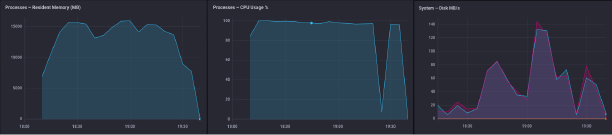
\includegraphics[scale=0.69]{rheos_read_mapper_chrom20_metrics}
    \centering
    \caption {System resource usage by Read Mapping Service during alignment of Chromosome 20 of NA12878 form GIAB.}
    \label{fig:rheos_read_mapper_chrom20_metrics}
\end{figure}

We next investigate the operation of the Locus Processor Service by simultaneously executing 4 instances of the service, one for each partition of Chromosome 20, on the stream data produced by the Read Mapping Service. We invoke the Locus Processor Service with the following set of parameters:
\\
\emph{
    service\\
-r data/reference/genome.fa\\
-g [20:1-20000000 | 20:20000001-40000000 | 20:40000001-60000000 | 20:60000001-63025520]\\
-k kafka:9092\\
--log\_level=DEBUG\\
--root\_log\_level=DEBUG\\
--logger\_type=stream\\
}

Here, each of the service instances has a separate partition and genomic region assigned via the -g parameter. This process completed in 29 minutes and 42 seconds running four instances simultaneously and took 0.452 seconds to process a single message on average, sending an average of 32908 updated loci for downstream processing per message. Consulting the operational metrics collected during the run (Figure \ref{fig:rheos_locus_processor_chrom20_metrics}) we see a fairly stable CPU and memory utilization profiles, however significant use of swap is observed (bottom right panel), indicating that if the amount of memory per process was increased, performance could be improved.


\begin{figure}[h!]
    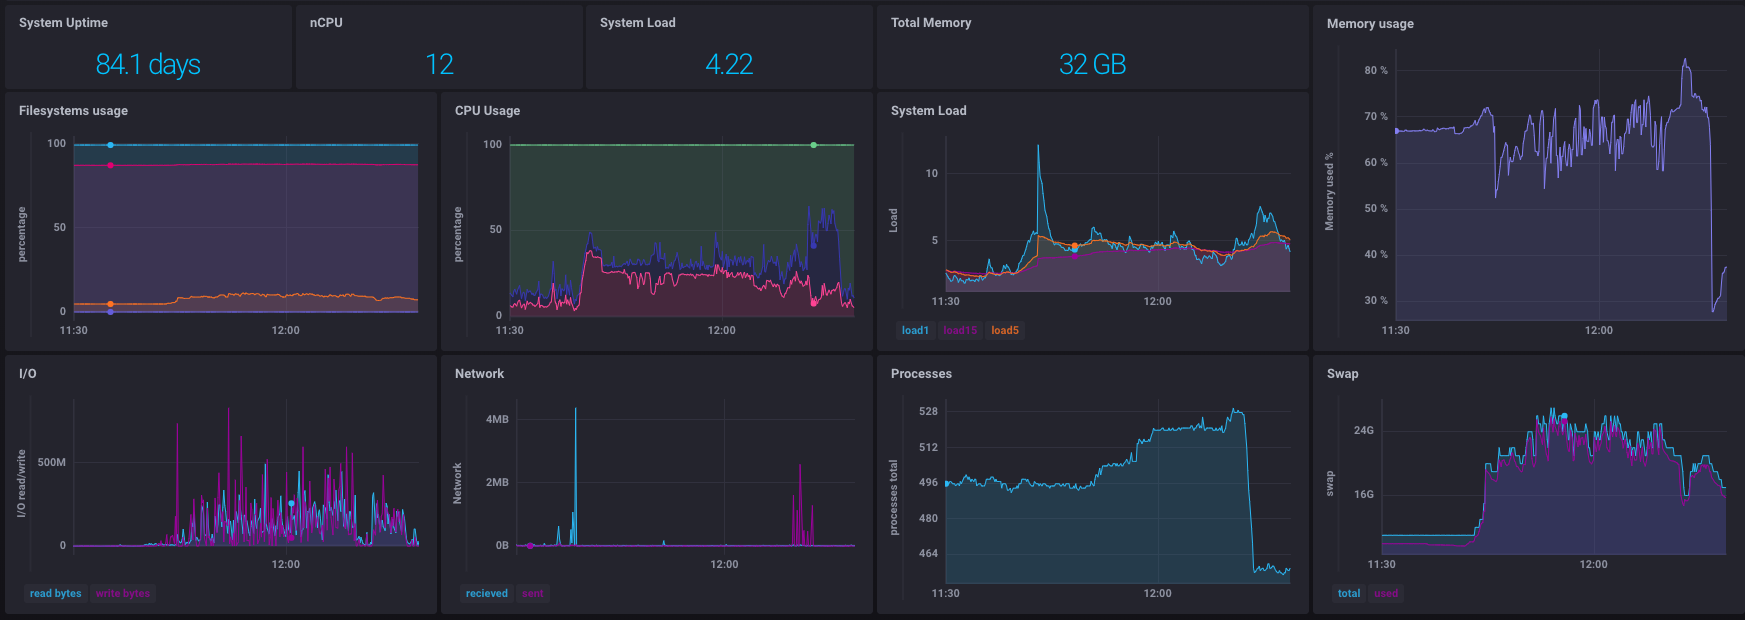
\includegraphics[scale=0.24]{rheos_locus_processor_chrom20_metrics}
    \centering
    \caption {System resource usage by Locus Processor Service during processing of Chromosome 20 of NA12878 form GIAB.}
    \label{fig:rheos_locus_processor_chrom20_metrics}
\end{figure}


We run a single instance of the Locus Saver Service to process locus updates with the following parameters:
\\
\emph{service\\
-k kafka:9092\\
-r redis-master -p 6379\\
--log\_level=DEBUG\\
--root\_log\_level=DEBUG\\
--logger\_type=stream}

This is a fairly lightweight service and takes 18 minutes and 58 seconds to process all of the messages produced by the  4 instances of Locus Processor and save them to Redis. 961 messages in total are processed, with average processing time of 0.72 seconds per message. Figure \ref{fig:rheos_locus_saver_chrom20_metrics} shows operational metrics collected from the service and the Redis server during the execution runtime. As can be seen, the execution fully utilizes the CPU of the service host (likely for serialization/deserialization of messages). Resources of the Redis server are only midly utilized indicating the ability to run several instances of the Locus Saver per instance of Redis. The bottom-left panel shows the impact of automated disk persistence of Redis in-memory data. This feature can be turned off to obtain higher throughput at the expense of lower availability, i.e. if Redis crashes data will need to be reprocessed.   

\begin{figure}[h!]
    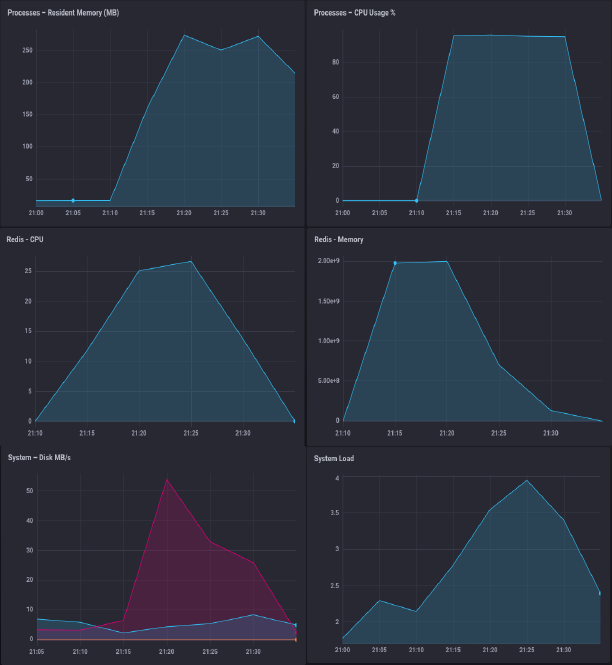
\includegraphics[scale=0.6]{rheos_locus_saver_chrom20_metrics}
    \centering
    \caption {System resource usage by Locus Saver Service during processing of Chromosome 20 of NA12878 form GIAB.}
    \label{fig:rheos_locus_saver_chrom20_metrics}
\end{figure}

The last component in the processing pipeline is the Variant Calling Service. We invoke this service with the following parameters:
\\
\emph{file\\
-g 20:1-63025520\\
-r redis-master -p 6379\\
--calling\_threshold=50\\
--max\_vqual=5000\\
-t variant\_caller\_pkg/variant\_caller/rheos\_vcf\_template.vcf\\
-o data/na12878\_20\_1\_63025520\_rheos\_latest.vcf\\
--log\_level=DEBUG\\
--root\_log\_level=DEBUG\\
--logger\_type=stream}

These parameters indicate that we are calling variants on the entirety of Chromosome 20, that we only include variants exceeding variant quality of 50 (i.e. 1 in 10000 variants is estimated to be a false positive), and with a variant quality ceiling of 5000 (if a variant has vqual >5000 it will be capped at 5000). Running a single instance of this service took 1 hour and 21 minutes to complete calling on the entire Chromosome 20 of the sample, evaluating 12754171 potential variant sites from Redis. Figure \ref{fig:rheos_variant_caller_chrom20_metrics} shows steady CPU utilization and relatively low memory use by the service (top panels), and steady but low CPU utilization, but high memory consumption by Redis (bottom panels), as expected.

\begin{figure}[h!]
    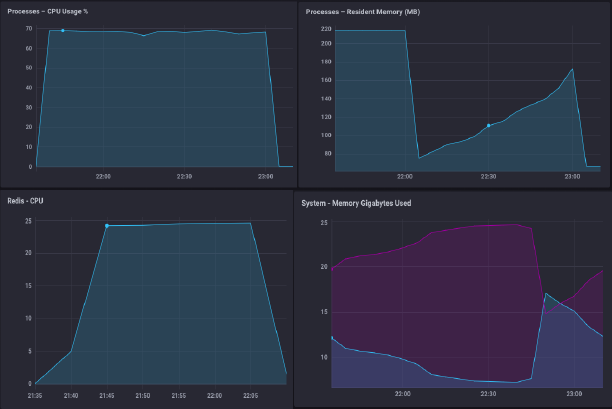
\includegraphics[scale=0.6]{rheos_variant_caller_chrom_20_metrics}
    \centering
    \caption {System resource usage by Variant Caller Service during processing of Chromosome 20 of NA12878 form GIAB.}
    \label{fig:rheos_variant_caller_chrom20_metrics}
\end{figure}

Using the procedure above we obtained a germline SNP callset containing 82576 germline variants. We compare the results of our callset to 2 other callsets for the same sample and genomic region:

\paragraph{freebayes} - To be able to best compare callsets, we took the same FASTQ file that has been used for the Rheos analysis, and aligned it against the GRCh37 reference genome using minimap2, producing a SAM file. We then sorted and compressed that SAM file using samtools, to produce a BAM file that can be used for variant calling by most tools.

We installed the latest version of freebayes\autocite{garrison2012haplotype} and invoked it with the following command:
\\
\emph{freebayes -r 20 -f reference/genome.fa \\
giab/RMNISTHS\_30xdownsample\_chr20.name\_sorted\_minimap.new\_rg.sorted.bam\\
 > tests\_latest/original/freebayes\_chr20\_minimap.vcf}

After filtering out indels we were left with a callset with 89704 SNPs.

\paragraph{GATK 4} - To obtain a GATK 4 callset. We installed and built the latest version of the GATK\autocite{mckenna2010genome} from github. Utilizing the same BAM file as was used for the freebayes callset, we invoked the GATK HaplotypeCaller with the following command:
\\
\emph{java -jar \$GATK HaplotypeCaller \\
-I ~/data/giab/RMNISTHS\_30xdownsample\_chr20.name\_sorted\_minimap.new\_rg.sorted.bam\\
 -R ~/data/reference/genome.fa  \\
 -O tests\_latest/gatk\_chrom20\_minimap.vcf  \\
 -pairHMM AVX\_LOGLESS\_CACHING \\
 -L 20
}

After removing indels we were left with a callset with 77762 SNPs.

We compared the Rheos callset to those produced by freebayes and GATK by running the Picard\autocite{Picard2018toolkit} tools' GenotypeConcordance utility, with the command:\\
\bigskip
\emph{ java -jar \$PICARD GenotypeConcordance \\
CALL\_VCF=tests\_latest/original/na12878\_20\_1\_63025520\_rheos\_latest.vcf  \\
TRUTH\_VCF=tests\_latest/gatk\_chrom20\_no\_indels.vcf   \\
O=tests\_latest/gatk\_to\_rheos/gatk\_to\_rheos \\
TRUTH\_SAMPLE=NA12878 \\
CALL\_SAMPLE=NA12878}
\bigskip
and a similar invocation for the freebayes to Rheos comparison.

The results were as follows:

\begin{table}[!ht]
    \centering
    \caption{Sensitivity and specificity of Rheos caller vs freebayes and GATK.}
    \label{tab:rheos_vs_fb_and_gatk}
    {\begin{tabular}{l | r | r}
    \toprule
    Rheos vs. & Sensitivity & Specificity \\
    \midrule
    freebayes & 0.988701 & 0.990385\\
    GATK & 0.984848 & 0.991597\\
    \bottomrule
    \end{tabular}}
\end{table}

While these results are quite good, and Rheos appears to capture the greatest majority of the signal that other well established tools do on the same data set, it is illuminative to manually consider a sample of loci where the callers disagree. Figure \ref{fig:rheos_snp_fns} shows three examples where variants called by GATK do not appear in the Rheos callset. 

In panel a) is a variant that is called a heterozygous SNP by GATK at the locus 930480 on Chromosome 20. Out of 14 reads 4 show the alternate allele T and GATK assigns a variant quality of 64.77. On the Rheos side, the variant was assigned a variant quality of 46.94, and consequently did not pass the quality threshold cutoff of 50 that was used when producing the callset. It is difficult to say based on this data whether this call is likely a true variant or not. Certainly, if a lower stringency cutoff was used the call would also be part of the Rheos callset.

In panel b) is a variant at position 20:2678084 that is called homozygous variant by GATK, but in fact, the coverage at this site is only 2 so GATK is making a call based on very limited information, and the call has a high probability of being a false positive in the GATK callset. Rheos attaches a probability of ~0.62 that the site is homozygous variant, and ~0.32 that the site is heterozygous variant. The overall variant quality however, is 12 on the account of the low number of observations and consequently the site does not pass the quality threshold.

In panel c) there are two adjacent SNPs in positions 20:18956622-18956623. The first of these is called by both variant callers, but the second is only present in the GATK callset. It is called a heterozygous SNP with 5 out of 19 reads showing the alternate A allele, and has a variant quality of 97.77. In the Rheos callset the variant is assigned a quality of 40.0 and does not pass through the quality cutoff. Because of the lower fraction of alternate allele observations than would be expected, it is possible that the site actually represents a somatic variant that is only present in the subset of the sample's cells.

A unifying theme of all of the false negative calls is that even though they are detected by Rheos, they end up below the quality threshold of 50 (one false variant in 100000). Using a less stringent filter will certainly increase sensitivity of the callset, although an approach for controlling the resultant increase in false positives is also required.

\begin{figure}[h!]
    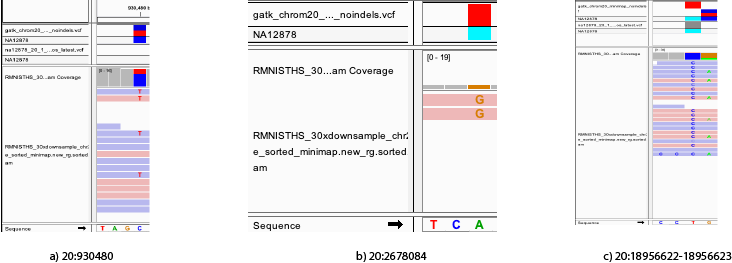
\includegraphics[scale=0.55]{rheos_snp_fns}
    \centering
    \caption {The Rehos germline deletion calling pipeline.}
    \label{fig:rheos_snp_fns}
\end{figure}

Figure \ref{fig:rheos_snp_fps} shows several examples of false positive calls, those that are detected as variant by Rheos but are not called by GATK. 

In panel a) we see a locus at 20:813667-813669 that is called as 3 adjacent SNPs by Rheos, whereas in GATK it is called a SNP adjacent to a complex variant. It is indeed probably a complex variant that extends to all 3 adjacent nucleotides, and there is evidence of both the presence of SNPs, as well as a small deletion at that locus. Since Rheos has no concept of indels or complex variants, these sites naturally end up as false positive SNP calls. 

In panel b) we see a locus at 20:2487891 that is called a heterozygous SNP by Rheos but is not present in the GATK callset. Rheos calls this site variant because there is a relatively large number (10/24) of alternate allele observations, although they are mostly of relatively low base quality (9 our of 10 reads have base quality between 6 and 8, implyiing probability of error between 15-25\% for each). Additionally, all of the alternatve allele observations fall on reads that map to the negative strand. This type of strand bias is a strong indicator of a false positive signal and is often used by variant filtering software to filter out false positives.

In panel c) we see a locus at 20:11298489 that is called homozygous variant in the Rheos callset, but is actually included as part of the neighbouring deletion by GATK. Indeed, this region is called differently by all three callers. GATK calls a 5bp indel at 11298472-11298476, followed by an 8bp indel at 11298482-11298489. Freebayes calls a 13bp indel 11298472-11298484, followed by a homozygous SNP at 11298489. And Rheos calls a bunch of SNPs inside the indel, since it presently has no concept of indels, followed by a homozygous SNP at 11298489. 

Two major sources of false positive signals are apparent for Rheos from this testing, areas around indels, and loci with many low quality bases. Both of these warrant further work to improve. 

\begin{figure}[h!]
    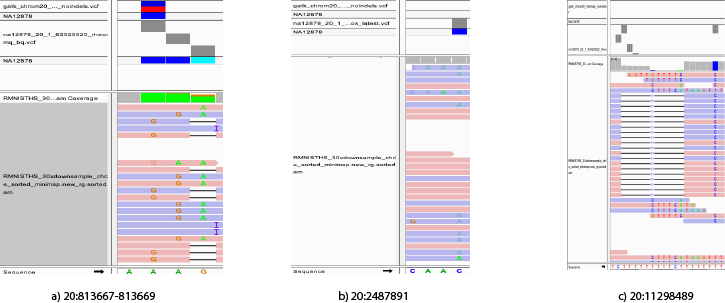
\includegraphics[scale=0.55]{rheos_snp_fps}
    \centering
    \caption {Three examples of false negative calls by Rheos, compared to GATK. a) Site with few, but high quality alternate allele observations. b) Site with very low coverage. c) Site of two adjacent SNPs, one of which has low variant quality.}
    \label{fig:rheos_snp_fps}
\end{figure}

Our testing of Germline SNP Calling with Rheos shows that this framewrok is capable of deployng scalably onto an academic cloud computing infrastructure and producing accurate results that are compatible with callsets produced by leading variant callers, while doing so in a streamlined, online manner that is not accessible to these other tools.

\subsection{Germline Deletion Calling}

For germline deletion calling we are interested in collecting discordantly mapped read pairs and performing clustering, and variant calling as described in Section \ref{sec:main_body_sv_calling}. We put together a Rheos pipeline shown in Figure \ref{fig:rheos_sv_calling_pipeline}. We use the same run of the Read Mapping Service as was used for germline SNP calling, but consume all of the reads from all mapped read partitions by the same single instance of the Insert Size Filtering Service.

\begin{figure}[h!]
    \includegraphics[scale=0.45]{rheos_sv_calling_pipeline}
    \centering
    \caption {Three examples of false positive calls by Rheos, compared to GATK. a) Site of a complex variant. b) Site with many low quality bases. c) Site of a SNP adjacent to an indel.}
    \label{fig:rheos_sv_calling_pipeline}
\end{figure}

We use the following settings for the Insert Size Filtering Service - accumulate 100000 read pairs for insert size estimation, keep read pairs with insert size > 5 * MAD (Median Absolute Deviation), that are both mapped, that map to the same contig, and that both have mapping quality >= 30. These settings result in 2663 read pairs passing through the Insert Size Filtering Service to the Insert Size Clustering Service. The total runtime was 4 minutes 32 seconds to process 13069 messages from 168 data partitions.

We use a single instance of the Insert Size Clustering Service applying the following settings - $min\_read\_support = 2$, $insert\_size\_threshold = 500$, indicating that we only want deletions that are supported by at least two discordant reads, and that we want to remove from a deletion's list of supporting reads, those that have $insert\_size > deletion\_width + 500$. We apply KDE clustering with a gaussian kernel, setting $bandiwdth = 100$. The runtime of the clustering and deletion calling was 17 seconds. Results of the clustering can be seen in Figure \ref{fig:kde}.

The initial calling produced a set of 36 putative deletions. Looking at the read pairs that support these deletions we observed that a deletion was supported, on average by ~121 read pairs. This is a very high number given that the total number of read pairs considered is 2663. This observation has led to the consideration of whether there is a significant number of potentially spurious read pairs with very long insert sizes that overlap many deletions, but do not actually contribute to the signal. We investigated the distribution of insert size widths in the data set, with results visible in Figure \ref{fig:insert_size_hist}. It is evident that even though the majority of insert sizes are relatively small - $< e^{10}$, there are over a hundred read pairs with insert size $> e^{14}$.

\begin{figure}[h!]
    \includegraphics[scale=0.6]{insert_size_hist}
    \centering
    \caption {A histogram of discordant read pair insert sizes on the log-log scale. X-axis is log(insert\_size), Y-axis is log(count).}
    \label{fig:insert_size_hist}
\end{figure}

We would like to investiage whether the large insert-size read pairs contribute significantly to signal identified by one-dimensional KDE, and indeed, whether they may cluster by themselves. To assess this, we introduce a second dimension of insert size to the original clustering, and perform a second round of KDE clustering in two dimensions, where each point was now of the form $(center, width)$. The results can be seen in Figure \ref{fig:2d_kde}. Here, the horizontal dimensions are insert size center and width, and the vertical dimension is density. We can see that most of the density still falls in the area of low width and along centre coordinate. We thus, believe that the very long insert sizes are not significant contributors to the detection of deletions that they overlap, and may be removed from the list of reads supporting those deletions. Indeed, when we remove these read pairs from our data set entirely and repeat the clustering, the results recapitulate those produced with the original data set, and only one fewer deletions is called. We thus introduce a width-based cutoff for reads supporting a deletion and set it to $deletion\_width + 500$, where all read pairs that have insert size greater than this cutoff are removed from the list of supporting reads. This results in a much more sensible average number of supporting reads per deletion, namely 9. We retain those deletions for our final callset that are supported by at least 2 read pairs, leaving 29 deletions in the final callset.

\begin{figure}[h!]
    \includegraphics[scale=0.6]{2d_kde}
    \centering
    \caption {2-D KDE estimate of insert size center and width, using a gaussian kernel with bandwidth 100.}
    \label{fig:2d_kde}
\end{figure}

We compare the results of this method with two other data sets. One is a set of structural variant calls produced by the GIAB consortium. We downloaded the file Personalis\_1000\_Genomes\_deduplicated\_deletions from ftp://ftp-trace.ncbi.nlm.nih.gov/giab/ftp/technical/svclassify\_Manuscript/Supplementary\_Information/. We then used the software package \emph{bedtools}\autocite{quinlan2010bedtools} to filter the data set to only include deletions on Chromosome 20 and those exceeding 500bp in length. The length trimming is necessary because the insert size based method of Rheos is limited to detecting deletions that are approximately equal to the $MAD * mad\_threshold$ in size. MAD is 131.95 in our data set and $mad\_threshold$ is 5. We take the cutoff at 500 since slightly smaller deletions can be detected, due to the overlap of multiple read pairs. This results in a callset of 26 deletions.

The other comparison data set is produced by calling variants with Delly\autocite{rausch2012delly}. We produce the callset by invoking Delly with the following command:

\emph{delly call -n -q 30 -s 5\\
 -g reference/genome.fa giab/RMNISTHS\_30xdownsample\_chr20.minimap.sorted.bam \\
 -o tests\_latest/delly\_chrom20\_dels\_minimap.vcf}

The flags supplied to Delly have been selected to mimic the cutoffs used for the Rheos caller. We then trim the callset to only include deletions that are not flagged as \emph{LowQuality}, and that are greater than 500 bp in length. This results in a callset of 25 deletions.

We used bedtools to compare the 3 callsets and produce the diagram of Figure \ref{fig:rheos_delly_giab_dels_venn} that shows the overlap between them. 83\% of the deletions called by Rheos are called in at least one of the other two callsets. This is a pretty satisfactory result as the Rheos callset only makes use of discordantly mapped reads at this time, while the other two callsets have been produced with methods that take advantage of split-reads and read depth analysis. 

\begin{figure}[h!]
    \includegraphics[scale=0.06]{rheos_delly_giab_dels_venn}
    \centering
    \caption {Venn diagram depicting overlap between the Rheos, Delly, and GIAB deletion callsets on Chromosome 20 of NA12878.}
    \label{fig:rheos_delly_giab_dels_venn}
\end{figure}

To assess the shortcomings of the Rheos deletion calling method we take a look at a sample of the deletions that are called by Rheos and not by other tools, and also those that are called by other tools but not by Rheos. Figure \ref{fig:rheos_sv_fps} shows the 5 deletion calls that were called only by Rheos. Out of these five calls, three (a), b), and e)) look like real deletions when the region is viewed with IGV. There is a clear depletion of reads in these regions compared to the surrounding regions and there are several discordantly mapped read pairs that overlay each region (3 each for deletions a), b), and c)). The region in panel b) is difficult to make calls in, because of the large number of low quality reads, with large portions clipped out of the aligment and the call is only supported by two read pairs so this can easily be a false positive. The region in d) is hard to judge, but can also be a false positive. 

\begin{figure}[h!]
    \includegraphics[scale=0.54]{rheos_sv_fps}
    \centering
    \caption {Visualization of the genomic regions that were called deletions by Rheos but not by other callers.}
    \label{fig:rheos_sv_fps}
\end{figure}

In Figure \ref{fig:rheos_sv_fns} we show several examples of deletion calls that were not part of Rheos' callset but were called by other tool. The deletions in panels a) and b) were part of the GIAB callset and part of the Delly callset. These look like very well defined deletions with a clear dropoff in read coverage, as well as split-reads flanking the deletion site. Since Rheos is currently not using read depth or split-reads, it was not able to make these calls. When looking at the deletion call in panel c) is not readily apparent that this is a deletion. Even though there are some split-reads at the flank, there is no dropoff in coverage. It may be that this is a false positive call in the GIAB callset. The deletion in panel d) was called by Delly, but is not in GIAB and was not called by Rheos. This region is difficult to judge by sight. There is clearly a small homzygous deletion in the left portion of the image, but the Delly deletion call spans the entire visible region. There is a clear difference in read depth visible, but only on one side of the region, the read depth towards the left is relatively constant. The only true variant in this region is likely the small deletion, but since it is too small for Delly to call, it is probably extending the call towards the right, thus creating a false variant. 

\begin{figure}[h!]
    \includegraphics[scale=0.54]{rheos_sv_fns}
    \centering
    \caption {Visualization of the genomic regions that were called deletions by both GIAB and Delly but not Rheos (a) and b)), GIAB but not Rheos or Delly (c)), Delly but not GIAB or Rheos (d)).}
    \label{fig:rheos_sv_fns}
\end{figure}

Based on the manual inspection of called regions that we performed, it appears that the true sensitivity and specificity of the Rheos deletion calling method would be underestimated by a direct comparison with the two other callsets, because they miss some calls that appear to be true, and because they make some calls that appear to be false. Overall, the currently implemented method of germline deletion calling in Rheos appears to be accurate, but will certainly benefit from the additional signal sources like split-reads and read depth that other tools make use of.

In our experimental validation work we were successfully able to deploy Rheos on cloud computing infrastructure using Google Kubernetes. We executed several real end-to-end variant calling use cases using a data set of ~4.7 GB in size. We successfully compared the results to the data produced by other well established variant callers and found them to be accurate. Future enhancements of the Rheos framework will surely improve both the scalability of the framework, as well as the accuracy of the callsets that it produces.
